\documentclass[12pt,letterpaper]{report} % use this when printing for thesis
% submission (single sided)
%\documentclass[11pt,letterpaper]{book} % use this instead of previous if double
% side wanted (for drafts), and some trees will be saved

% To make bibliography title all caps
\renewcommand\bibname{\vspace{0.2in} \Large  BIBLIOGRAPHY}


%\textwidth 6.5in \oddsidemargin 0in \evensidemargin 0in \textheight
%8.5in \topmargin -3.5in

\usepackage{amsmath}
\usepackage{amssymb}
\usepackage{amsthm}
%\usepackage{doublespace}    % use this package if compiling from UNIX (and comment setspace)
\usepackage{setspace}       % use this package if compiling from Windows using MikTex or LiveTex and comment doublespace
\usepackage{epsfig}
\usepackage{unh_thesis}
%\usepackage{harvard}
\usepackage{times}
\usepackage[bookmarks=true, colorlinks=true, citecolor=blue,
urlcolor=blue, linkcolor=black]{hyperref}

\usepackage{todonotes}

\usepackage{mathptmx} % rm & math
\usepackage[scaled=0.90]{helvet} % ss
\normalfont
\usepackage[T1]{fontenc}
\usepackage[scaled=0.9]{inconsolata}

\usepackage[T1]{fontenc}
\usepackage[left=1.55in,top=1.1in,right=1.1in,bottom=1in]{geometry}    %HP
% laserjet 3600
%\usepackage[colorlinks=true, pdfstartview=FitV, linkcolor=black,
% citecolor=black, urlcolor=black]{hyperref}
\usepackage{graphicx}
\usepackage[numbers]{natbib} % packages added by Gopal
\usepackage{lscape} \usepackage{multirow} \usepackage{supertabular}
\usepackage{rotating} %\usepackage{pstricks}
\usepackage{longtable} \usepackage{threeparttable} \usepackage{mathtools}
\usepackage{relsize} %\usepackage{caption}
%\DeclareMathSizes{12}{20}{14}{10}  % For size 12 text
%\DeclareMathSizes{11}{19}{13}{9}   % For size 11 text
\DeclareMathSizes{10}{18}{12}{8}    % For size 10 text
% This package and new command were added by Gopal to use in the creating long
% tables, tables spanning multiple pages. %The issue  was that pre-defining the
% parboxes for a long table automatically justified the text. This command keeps
% %the box sizes and aligns the text to the left of the box. so instead of "p"
% for defining a parbox in a table an "x" is used which is \raggedright (means
% flushes to left)
\usepackage{array} \newcolumntype{x}[1]{%
>{\raggedright\hspace{0pt}}p{#1}}%

%My own added commands
    \newcommand{\ee}{\end{equation}}
    \newcommand{\be}{\begin{equation}}
    \newcommand{\bi}{\begin{itemize}}
    \newcommand{\ei}{\end{itemize}}
    \newcommand{\bc}{\begin{center}}
    \newcommand{\ec}{\end{center}}
    \newcommand{\mc}{\multicolumn}

    \newcommand{\nm}{{\it nautical miles}}
    \newcommand{\ms}{${\rm m\,s^{-1}}$}
    \newcommand{\mms}{${\rm mm\,s^{-1}}\,$}
    \newcommand{\cms}{${\rm cm\,s^{-1}}\,$}
    \newcommand{\kgm}{${\rm kg\,m^{-1}}\,$}
    \newcommand{\kgmmm}{${\rm kg\,m^{-3}}\,$}
    \newcommand{\dgr}{$^{\circ}$}
    \newcommand{\mmn}{$\rm m^{-2}$}
    \newcommand{\mn}{$\rm m^{-1}$}

    \newcommand{\DP}[2]{\frac{\partial #1}{\partial #2}}
    \newcommand{\DF}[2]{\frac{#1}{ #2}}

    \def \p{\partial}
    \def \d{\mathrm{d}}
    \def \D{\mathrm{D}}

%Commands related to figures
%    \setlength{\abovecaptionskip}{-1mm}
%    \renewcommand\floatpagefraction{.9}
%    \renewcommand\topfraction{.9}
%    \renewcommand\bottomfraction{.9}
%    \renewcommand\textfraction{.1}
%    \setcounter{totalnumber}{50}
%    \setcounter{topnumber}{50}
%    \setcounter{bottomnumber}{50}
%%%

\pagestyle{plain} % Puts page number on the bottom over the whole thesis


%% Code syntax higlighting

\usepackage{listings}
\usepackage{color}

% Subfigures/captions
%\usepackage{caption}
%\usepackage{subcaption}

\definecolor{mygreen}{rgb}{0,0.6,0}
\definecolor{mygray}{rgb}{0.5,0.5,0.5}
\definecolor{mymauve}{rgb}{0.58,0,0.82}

\lstset{frame=single,
    language=C++,
    aboveskip=3mm,
    belowskip=3mm,
    showstringspaces=false,
    columns=flexible,
    basicstyle=\ttfamily,
    numbers=none,
    numberstyle=\tiny\color{mygray},
    keywordstyle=\bfseries\color{blue!40!black},
    commentstyle=\color{gray},
    stringstyle=\color{mygreen},
    otherkeywords={for,if,else},
    breaklines=true,
    breakatwhitespace=true,
    tabsize=4,
    escapeinside={\%*}{*)},
    keepspaces=true,
    captionpos=b
}


% BIBLIOGRAPHY STYLE:
%
%\bibliographystyle{myunsrt}
%\bibliographystyle{unsrt} % this was in Gagik's
%\bibliographystyle{apsrev}
%\bibliographystyle{harvard}
%\bibliographystyle{abbrvnat}
%\bibliographystyle{abbrv}


\makeatletter
    \def\thebibliography#1{\chapter*{REFERENCES\@mkboth
      {REFERENCES}{REFERENCES}}\list
      {[\arabic{enumi}]}{\settowidth\labelwidth{[#1]}\leftmargin\labelwidth
    \advance\leftmargin\labelsep
    \usecounter{enumi}}
    \def\newblock{\hskip .11em plus .33em minus .07em}
    \sloppy\clubpenalty4000\widowpenalty4000
    \sfcode`\.=1000\relax}
    \makeatother


\begin{document}

\listoftodos

% FRONTMATTER - Includes title page, acknowledgments, abstract, etc
%%%%%%%%%%%%%%%%%%%%%%%% frontmatter %%%%%%%%%%%%%%%%%%%%%%%%%%%

%           TITLE PAGE

\title{On the use of \LaTeX for thesis writing}

\author{Jane Doe}
\prevdegrees{B.S., University of New Hampshire, Durham, NH, USA, 2013} \major{Mechanical Engineering}
\degree{Master of Science} \degreemonth{September} \degreeyear{2015}
\thesisdate{\today} \DOCUMENTtype{THESIS}
\documenttype{Thesis}
\maketitle

%%%%%%%%%%%%%%%%%%%%%%%%%%%%%%%%%%%%%%%%%%%%%%%%%%%%%%%%%%%%%%%%%
%           THE COMMITTEE


\newpage
\thispagestyle{empty}

%\vspace{2mm}
\begin{tabular}{l}
\\
\vspace{7.5mm}

This thesis has been examined and approved.

\end{tabular}

%\begin{minipage}[t]{16.5cm}
%\vspace{10mm}
\begin{flushright}

\begin{singlespace}
\tabletail
   {\hline \multicolumn{1}{r}{\emph{}}\\}
\tablelasttail{}
\begin{supertabular}{p{13cm}}
%      \begin{tabular}{l}
         %\vspace{10mm}\\
      \hline
         Dissertation Director, Kenneth C. Baldwin \\
         Professor of Mechanical Engineering and Ocean Engineering \\
        \vspace{8.5mm}\\
      \hline
         Dissertation Co-Director, Jeffrey S. Melton \\
     Research Assistant Professor of Civil/Environmental Engineering \\
        \vspace{8.5mm}\\
      \hline
         Lloyd C .Huff \\
        Research Professor of Ocean Engineering \\
        \vspace{8.5mm}\\
      \hline
         Larry A. Mayer \\
         Professor of Ocean Engineering and Earth Sciences\\
        \vspace{8.5mm}\\
      \hline
         M. Robinson Swift \\
        Professor of Mechanical Engineering and Ocean Engineering\\
        \vspace{8.5mm}\\
      \hline
         Pedro A. De Alba\\
         Professor of Civil Engineering and Ocean Engineering \\
          \vspace{8.5mm}\\
      \hline
         Igor I. Tsukrov \\
         Associate Professor of Mechanical Engineering and Materials Science \\
                 \vspace{8.5mm}\\
%    \end{tabular}
    \end{supertabular}

    \begin{tabular*}{3in}{l}
      \hline
        Date
    \end{tabular*}

\end{singlespace}
\end{flushright}

%%%%%%%%%%%%%%%%%%%%%%%%%%%%%%%%%%%%%%%%%%%%%%%%%%%%%%%%%%%%%%%%
%           DEDICATION PAGE



%\begin{figure*}[htbp] \centering
%\includegraphics[angle=0,width=0.6\textwidth]{figs/sans3}
%\end{figure*}

%\begin{figure*}[htbp] \centering
%\includegraphics[angle=0,width=1.1\textwidth]{figs/sans_trans}
%\end{figure*}

% \begin{center}
\par \noindent
%Then was not non-existent nor existent, there was no realm of air, no sky beyond it.
\par \noindent
%What covered in, and where? and what gave shelter? Was water there, unfathomed depth of water?
%\par \noindent
%There was neither non-existence nor existence then.\\
%There was neither the realm of space nor the sky which is beyond.\\
%What stirred? Where? In whose protection?\\
%Was there water, unfathomably deep?
%
%- Nasadiya Sukta, Rig Veda (Mandala 10, Hymn 129) (\citet{doniger81})
% %\end{center}
  \begin{dedication}
\begin{minipage}[t]{13cm}
\bc
    \begin{tabular}{c}


        \\[3cm]
        For Mom.

    \end{tabular}
    \ec
\end{minipage}


\end{dedication}

%%%%%%%%%%%%%%%%%%%%%%%%%%%%%%%%%%%%%%%%%%%%%%%%%%%%%%%%%%%%%%%%
%           ACKNOWLEDGMENTS PAGE
\acknowledgments \par \indent
This work would not have been possible without advice, support and assistance
provided by several individuals.
\endacknowledgments

%%%%%%%%%%%%%%%%%%%%%%%%%%%%%%%%%%%%%%%%%%%%%%%%%%%%%%%%%%%%%%%%

\tableofcontents

\listoftables

\listoffigures

%%%%%%%%%%%%%%%%%%%%%%%%%%%%%%%%%%%%%%%%%%%%%%%%%%%%%%%%%%%%%%%%
%           ABSTRACT PAGE (REQUIRED)
\begin{abstractpage}
%\indent
\par \indent
This is the abstract.
\end{abstractpage}


%%%%%%%%%%%%%%%%%%%%%%%%%%%%% end %%%%%%%%%%%%%%%%%%%%%%%%%%%%%%%


% just in case you want to reduce the size of the thesis for printing purposes,
% need to comment "singlespace" from bibliography
%\begin{singlespace}

\pagenumbering{arabic}

% Introduction setting up motivation, goals, requirements
\chapter{Introduction}

With the threat of anthropogenic climate change and the looming end to fossil
fuel supplies, human civilization must reduce carbon emissions \cite{Hansen2013}
and transition to a fully sustainable energy portfolio. Towards this end,
natural fluid flows such as wind and water in river and tidal flows---a.k.a.
marine hydrokinetic (MHK) energy---can contribute. It is estimated that there is
11,000 and 4,200 GW of wind power capacity potential from on- and offshore in
the US, respectively \cite{Lopez2012}, while there is approximately 50 GW of
technically available MHK power in the US \cite{Haas2011, Jacobson2012,
    Haas2013}. For reference, the United States produced on average about 438 GW of
electric power in 2013, and only 13\% of this was from renewable
sources~\cite{EIA2015}, which shows just how much work there is left to be done.

A turbine is the most common type of machine for extracting renewable energy
from fluid flows, converting the energy to shaft work as the fluid applies
torque on the rotor. Wind turbine designs have matured a lot over the past
couple decades, to the point where they are not changing much conceptually,
though they are pushing forward by increasing size. MHK turbine designs on the
other hand are quite immature despite taking heavy influence from wind
technology.

Turbine rotor concepts can essentially be divided into two classes---axial-flow
and cross-flow---describing the relative orientation of the axis to the nominal
flow direction. The ubiquitous horizontal-axis wind turbine (HAWT) is an example
of an axial-flow turbine (AFT), while the egg-beater shaped Darrieus
vertical-axis wind turbine (VAWT), patented in 1931 \cite{Darrieus1931}, is an
example of a cross-flow turbine (CFT). Note that a cross-flow turbine can accept
flow from any direction perpendicular to its rotation, meaning the axis can be
horizontal, vertical, or anything in between.

The most well-know CFT, the Darrieus vertical-axis wind turbine, examples of
which are shown in Figure~\ref{fig:Darrieus}, was developed thoroughly in the
late 1970s through the early 1990s by groups including Sandia National
Laboratories (SNL) in the US and the National Research Council (NRC) in Canada
\cite{Para2002}. Sandia's efforts culminated in their 34 m Test Bed, shown in
Figure~\ref{fig:Sandia-34m}. The lessons and knowledge gained from this research
turbine were used to create a ``point design'' for commercialization
\cite{Sutherland2012}. Turbine developer FloWind used the point design and
technical guidance from SNL to develop three-bladed composite rotors for their
fleet of VAWTs, shown in Figure~\ref{fig:FloWind}, resulting in moderate
commercial success. The highest power output of any VAWT---in the 1--3 MW
range---was achieved by the Canadian Lavalin Eole 64 m Research Turbine,
constructed in 1986 \cite{Para2002}, and shown in Figure~\ref{fig:Eole}.

\begin{figure}
    \centering

    \begin{subfigure}[b]{0.595\textwidth}
        \centering
        
        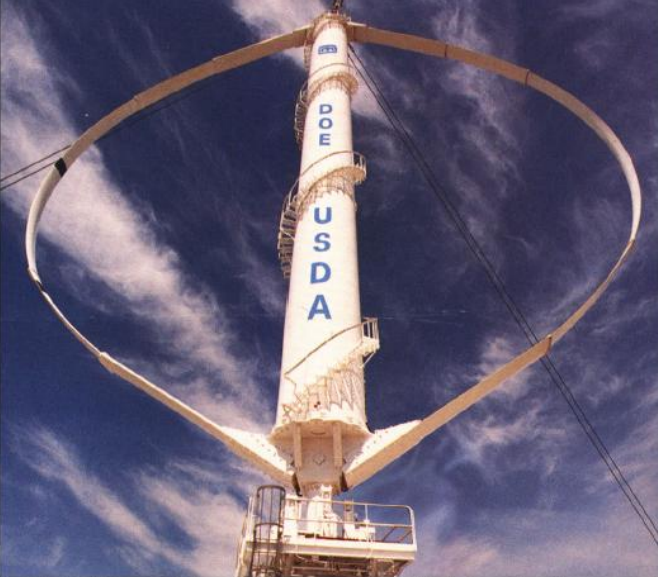
\includegraphics[width=\textwidth]{Murray2011-34m}
        
        \caption{Sandia 34 m Test Bed, from \cite{Murray2011}.}
        
        \label{fig:Sandia-34m}
    \end{subfigure}
    \hfill
    \begin{subfigure}[b]{0.355\textwidth}
        \centering
        
        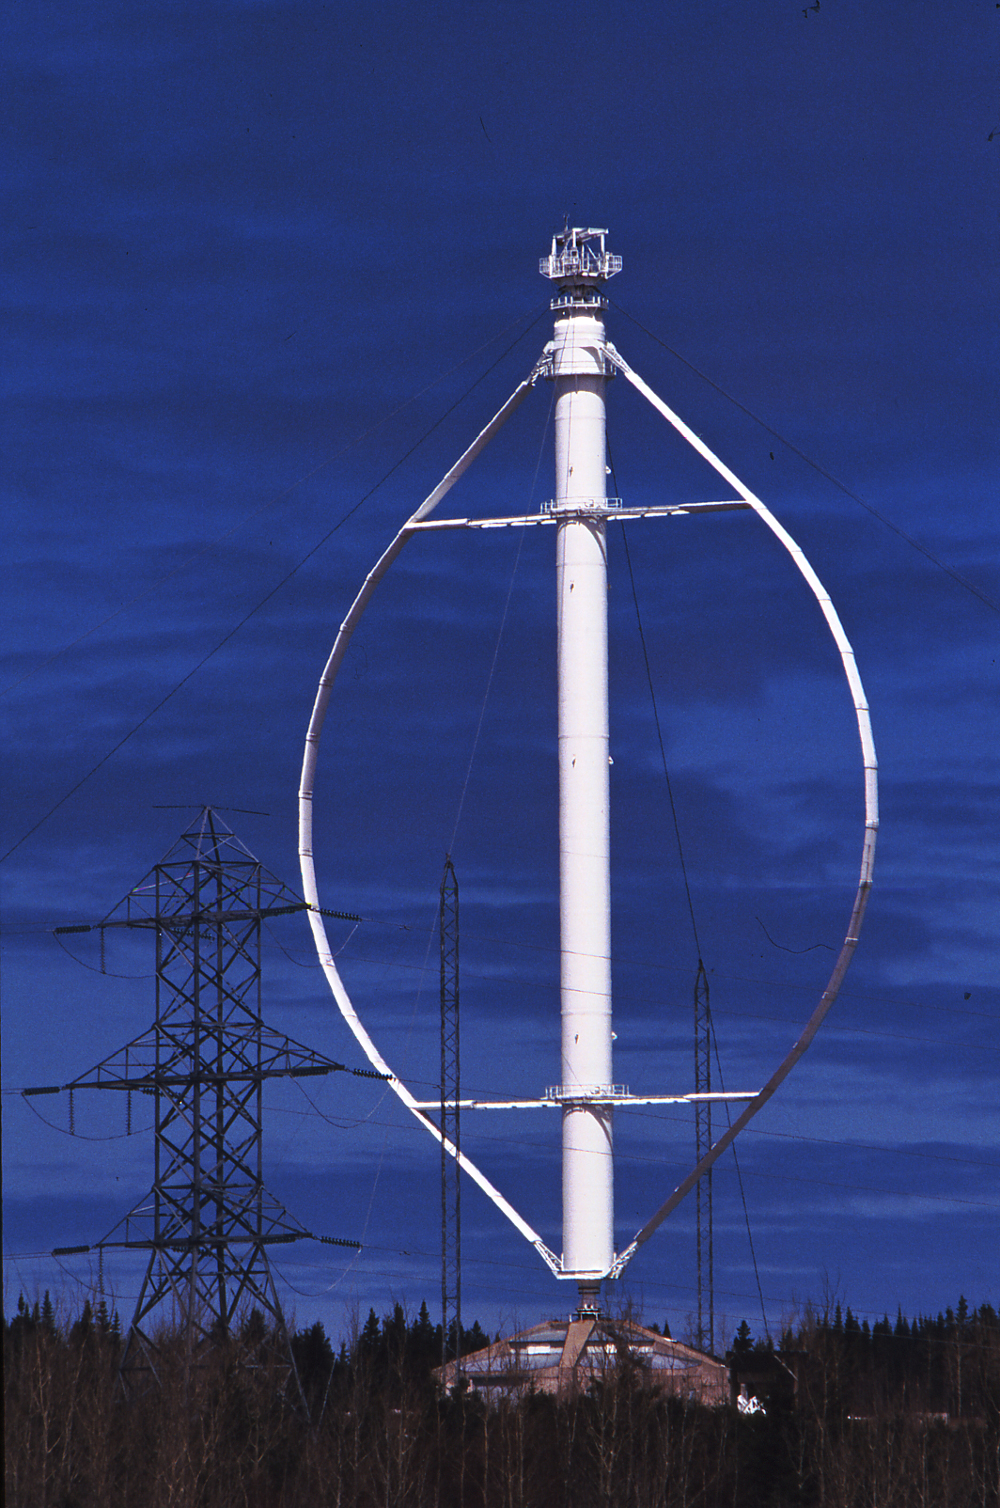
\includegraphics[clip, trim=0 0 0 0.05in, width=\textwidth]{Eole}
        
        \caption{Lavalin Eole 64 m VAWT. Photo by Paul Gipe. All rights
            reserved.}
        
        \label{fig:Eole}
    \end{subfigure}
    
    \begin{subfigure}[b]{0.8\textwidth}
        \centering
        
        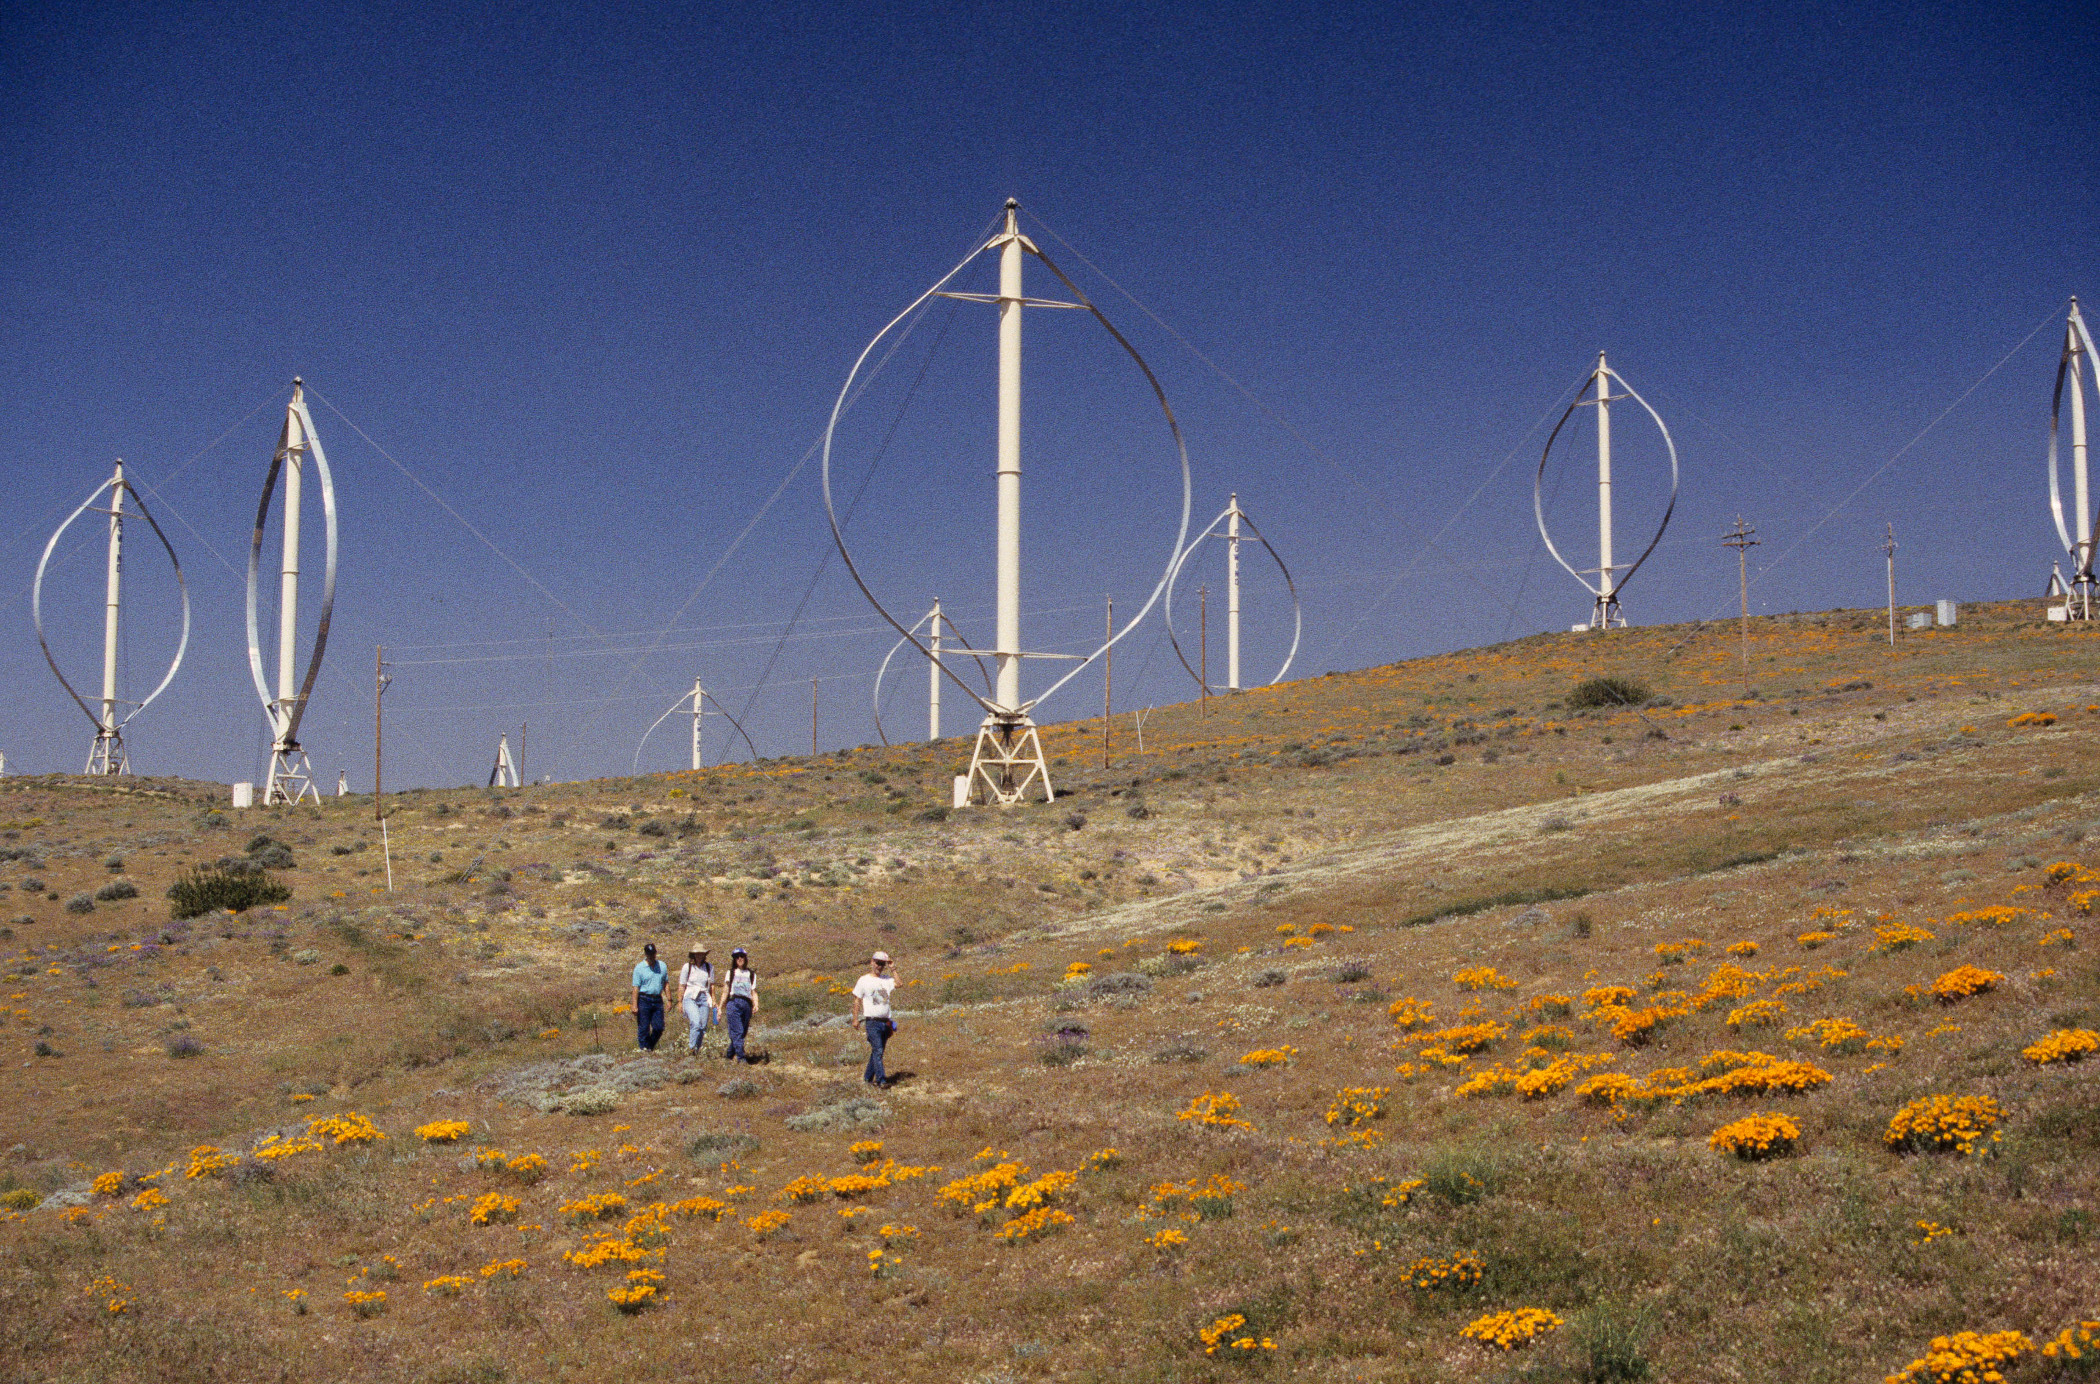
\includegraphics[width=\textwidth]{flowind}
        
        \caption{FloWind VAWT array. Photo by Paul Gipe. All rights reserved.}
        
        \label{fig:FloWind}
    \end{subfigure}
    
    \caption{Large scale Darrieus wind turbines: Sandia 34 m Test Bed (a),
        Lavalin Eole 64 m (b), and FloWind VAWT array (c).}
    
    \label{fig:Darrieus}
\end{figure}

Ultimately the three-bladed, horizontal-axis propeller-type axial-flow turbine
(AFT) concept---shown in Figure~\ref{fig:AFT} has became the design of choice
for large scale onshore wind---and for good reasons. Axial-flow turbines are
easier to analyze since their operating principles can be though of as an
essentially steady flow over a foil before stall. AFTs also have the benefit of
research ``inertia''---a lot has been invested and a lot of knowledge has
accumulated already. As a result, the designs are quite mature, for wind energy
at least. In contrast, the CFT has been studied and applied significantly less,
though there have been cases where CFTs have performed nearly equivalently well
as AFTs. However, CFTs are harder to design, since their blades are constantly
changing their angles of attack throughout the turbine's rotation, often
undergoing dynamic stall as part of normal operation \cite{Para2002}. Beside
their unpredictability, the highly oscillatory blade loading presents
significant design challenges for avoiding fatigue---a main cause for failure or
premature retirement of the large Darrieus wind turbines.

\begin{figure}[ht]
    \centering
    
    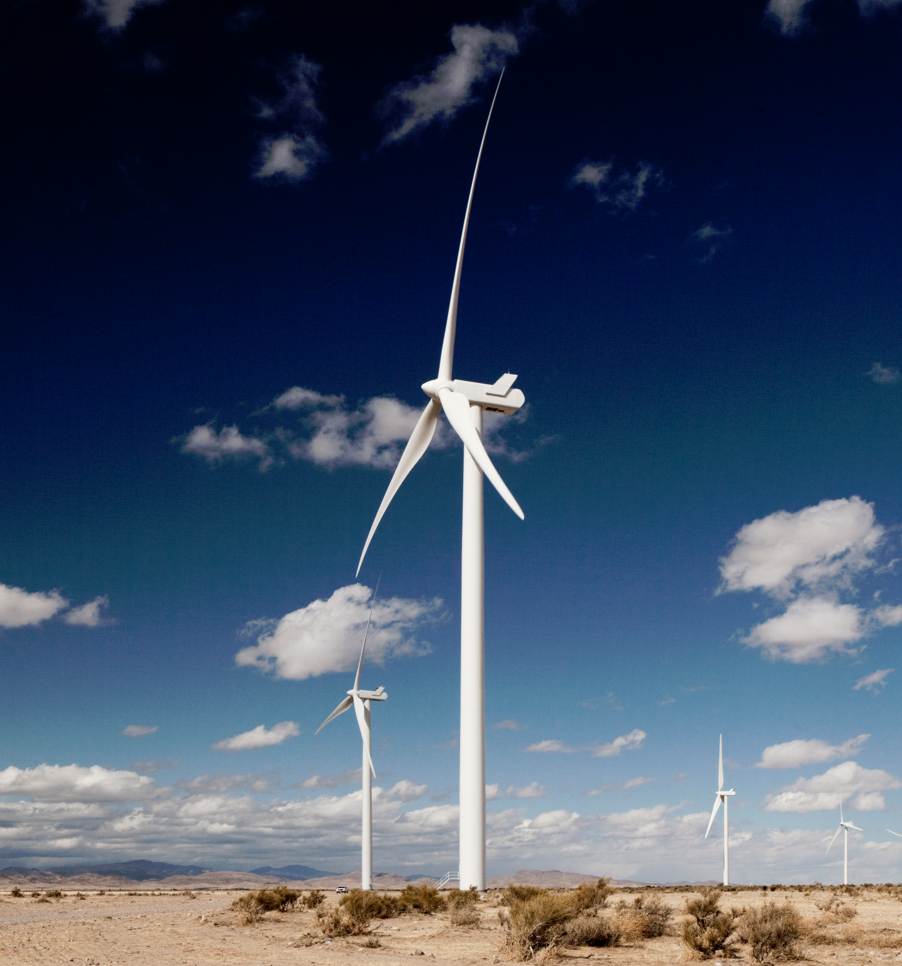
\includegraphics[width=0.7\textwidth]{Vestas-V100}
    
    \caption{Vestas V100 1.8 MW three-bladed axial-flow, a.k.a horizontal-axis
        wind turbine. Courtesy of Vestas Wind Systems A/S.}
    
    \label{fig:AFT}
\end{figure}

Despite their shortcomings, CFTs still may be valuable in some cases. They are
simpler, omni-directional machines, which negates the need for yawing and
pitching mechanisms. There were considerations in the 2010s by DEEPWIND in
Europe \cite{Paulsen2011} and SNL \cite{Sandia2012} in the US for using large
scale floating VAWTs for offshore wind, since along with the
omni-directionality, a vertical shaft allows placement of the generator and
gearbox lower in the machine, which lowers center of gravity. In the onshore
wind arena, CFTs show promise for projects where space is limited, e.g., urban
environments, as adjacent turbines sometimes interact ``constructively'' to
increase each other's power outputs \cite{Li2010}---a trait not possessed by
AFTs. A group from the California Institute of Technology has shown that arrays
of VAWTs can potentially provide an order-of-magnitude increase in the power
output per land area of a wind turbine array, since the devices can be spaced
more closely than HAWTs \cite{Dabiri2011}. Field measurements have shown that
their wakes recover more quickly than those of AFTs, and this cannot be entirely
attributed to higher turbulence generation \cite{Kinzel2012}. This phenomenon is
investigated in later chapters.

In the built, i.e., suburban and urban environments, wind resources are less
understood, more variable in terms of direction, speed, and turbulence levels
\cite{Smith2012}. Kooiman and Tullis \cite{Kooiman2010} observed that a
cross-flow turbine in an urban environment was indeed insensitive to changes in
wind direction, and was only adversely affected by temporal variations in wind
speed when turbulence intensity was above 15\%. The lack of need for yawing can
help lower cost of energy from CFTs versus AFTs by reducing complexity, e.g., by
eliminating slip rings. Cross-flow turbines may also have an advantage in the
urban environment since they must be designed for high fatigue loads anyway.
Recently, the Eiffel tower in Paris, France has been outfitted with two 5.3 m
tall, 3.2 m diameter helical vertical-axis cross-flow turbines, which will
produce at least 10 kWh/yr, or approximately 1 kW on average, which is expected
to power the entire first floor of the facility \cite{Lott2015}.

For MHK development, a field much less mature than wind power, the cross-flow
turbine concept is playing a major role thanks to its omni-directionality and
flexibility with respect to frontal area shape, allowing for more precisely
tuned fitment in channels with complex bathymetry or installed structures.
Chosen by the Ocean Renewable Power Company (ORPC) for their TidGen design, a
cross-flow turbine was the first grid-connected tidal energy device in the US,
which was installed in Cobscook Bay, ME \cite{ORPC2012}. Today, ORPC is working
on improving their turbine's performance, and planning for the installation of 4
more turbines \cite{Nelson2013}. 

CFTs are also being considered for micropower applications, such as powering
remote underwater instrumentation packages that currently rely on batteries
\cite{Polagye2013b}. They are also being used in riverine applications, for
example, in ORPC's RivGen project in the Kvichak River just downstream of the
village of Igiugig, AK~\cite{Forbush2015}, and the Rosa canal in Yakima, WA
\cite{Gunawan2014}. 

In general, the failure of cross-flow turbines in the large scale wind industry
can be largely attributed to less-than-adequate predictive capability in the
engineering process, i.e., issues with low performance and fatigue could be
overcome. In order for modern cross-flow turbines to be effective, these
capabilities must be enhanced, for both individual devices and arrays, which is
a primary motivation for this research.


\section{Principles of cross-flow turbine operation}

Blade element theory, originally conceived by
Drzewiecki~\cite{Drzewiecki1892,Drzewiecki1920}, is the analysis of a rotor or
propeller as a collection of 2-D foil sections, or blade elements, and can be
employed to obtain a simplified view of the kinematics and dynamics of a CFT.
Figure~\ref{fig:vectors} shows the relevant velocity and and force vectors on a
CFT blade element. The relative velocity and angle of attack $\alpha$ are
calculated by adding the inflow velocity vector to the opposite of the blade
element velocity $\omega R$, where $\omega$ is the shaft angular velocity and
$R$ is the element radius. In the relative velocity coordinate system, the lift
and drag are then oriented normal and tangential to the relative velocity,
respectively. These forces ultimately produce the shaft torque, and in turn the
shaft power.

\begin{figure}[ht]
    \centering
    
    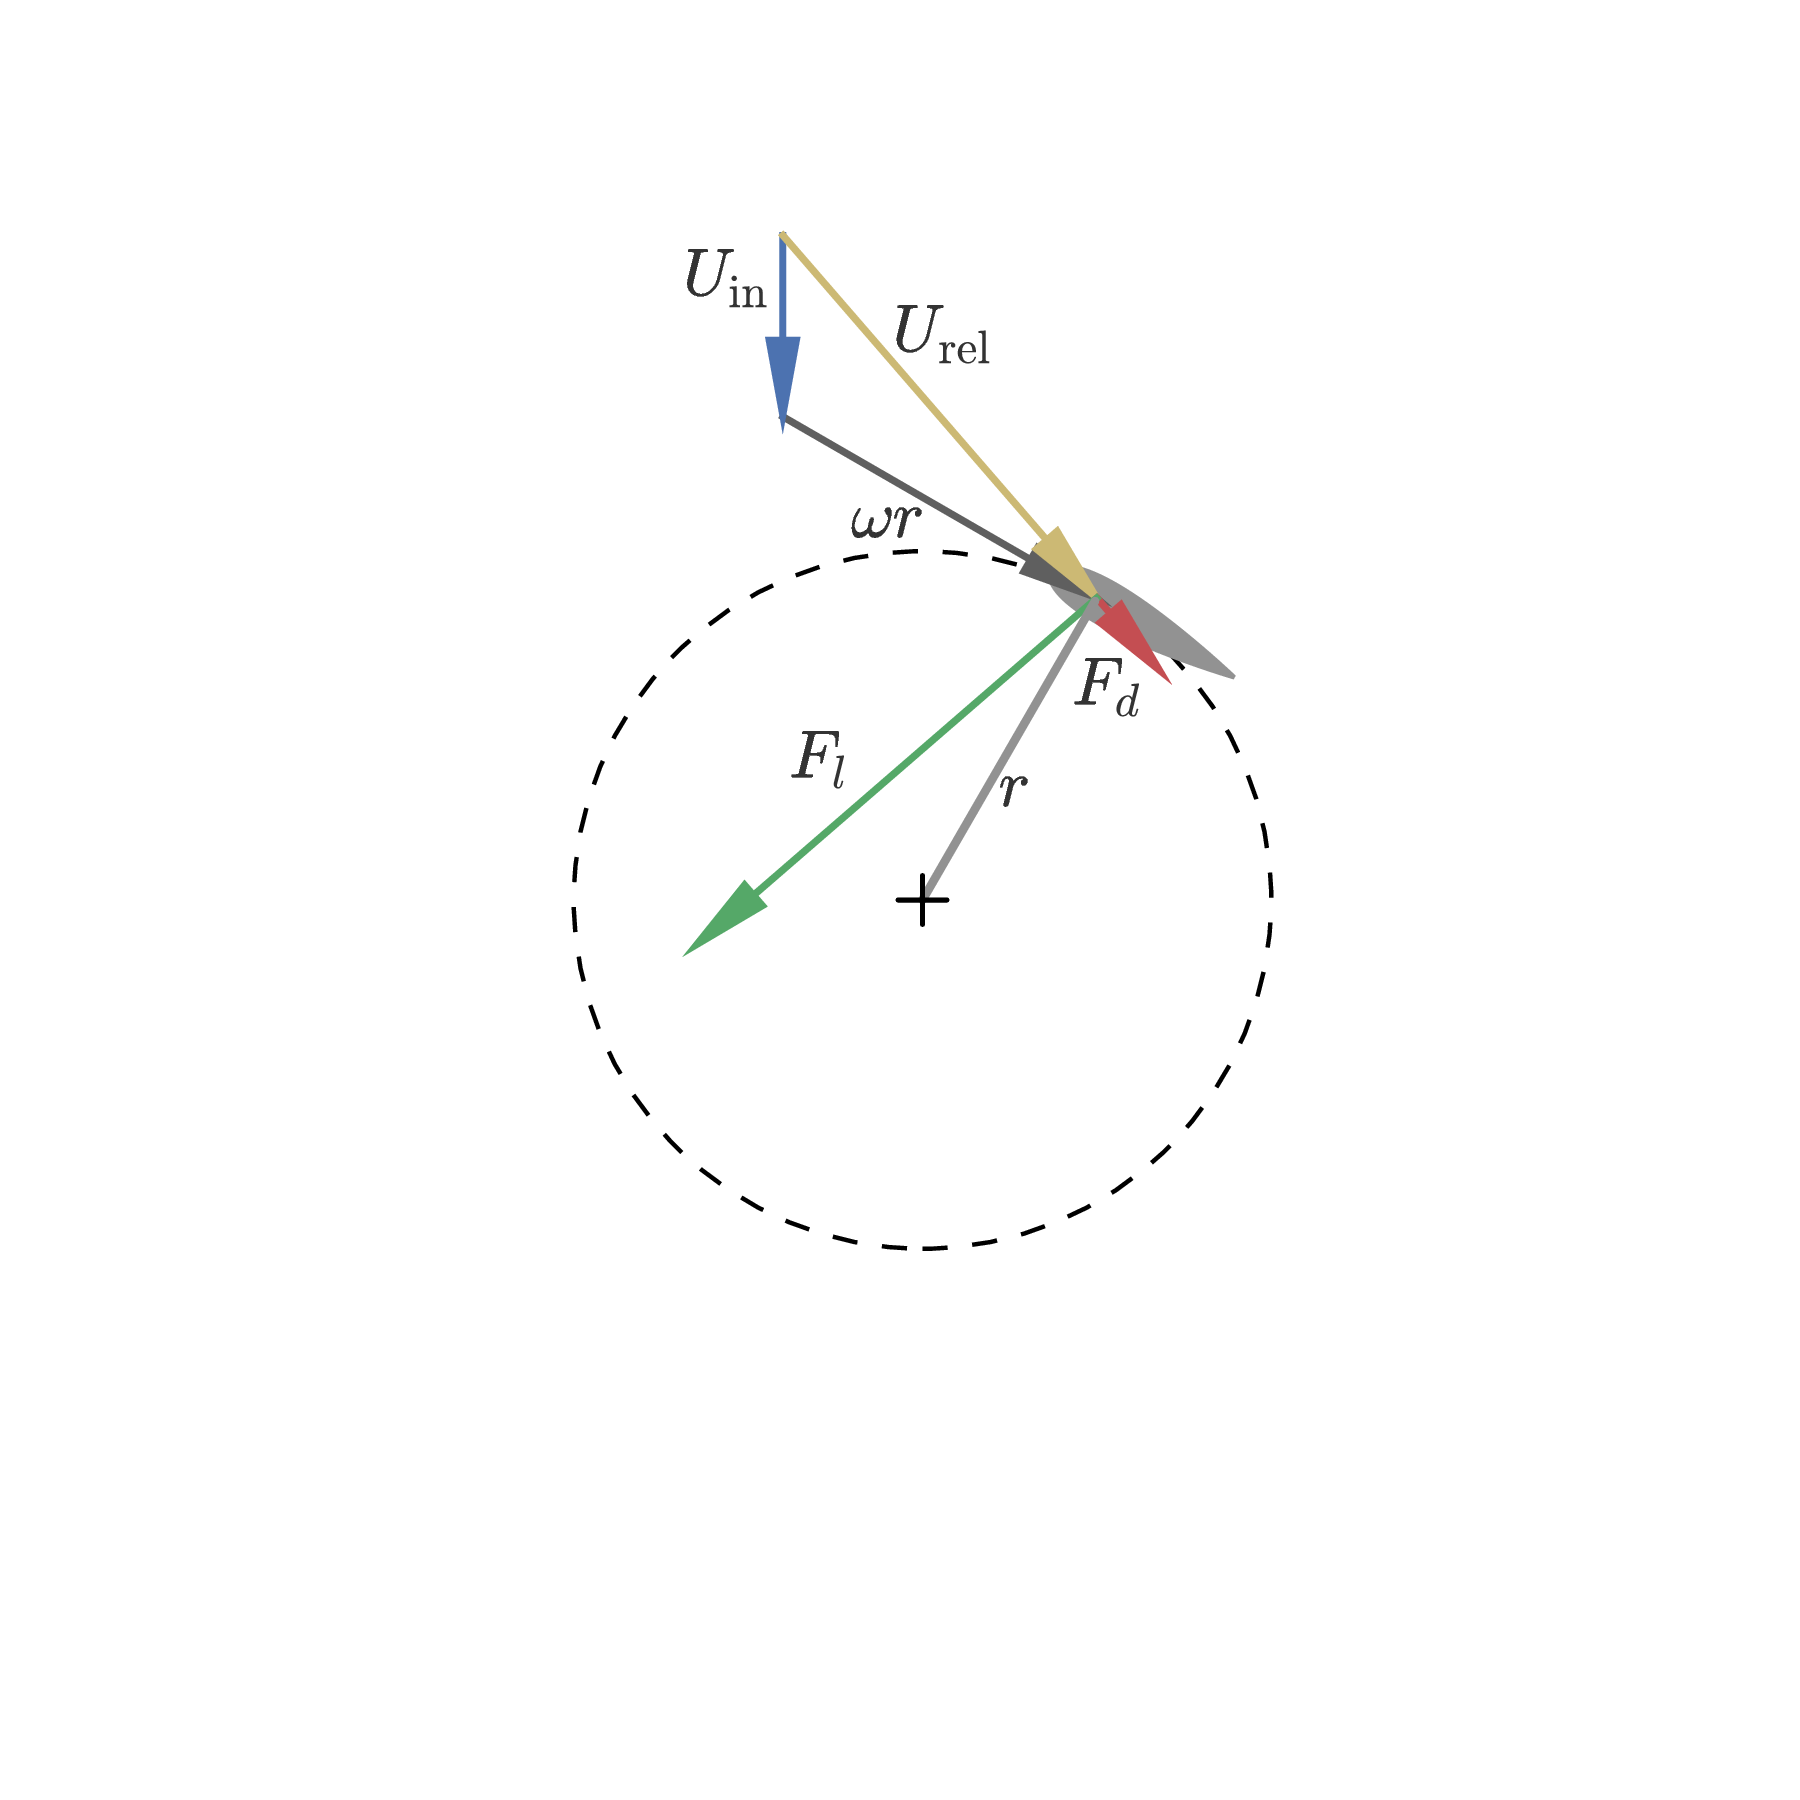
\includegraphics[clip, trim=1in 1.5in 1in 0.5in,
    width=0.6\textwidth]{figures/CFT-vectors_cft-vectors}
    
    \caption{Vector diagram of velocity and forcing on a cross-flow turbine
        blade element.}
    
    \label{fig:vectors}
\end{figure}

The shaft's angular velocity is nondimensionalized as the tip speed ratio
\begin{equation}
    \lambda = \frac{\omega R}{U_\infty},
    \label{eq:lambda}
\end{equation}
where $U_\infty$ is the free stream velocity.
Torque $T$ is characterized by the nondimensional torque coefficient 
\begin{equation}
    C_T = \frac{T}{\frac{1}{2} \rho A R U_\infty^2},
    \label{eq:ct}
\end{equation}
where $\rho$ is the fluid density and $A$ is the turbine's frontal area.
Similarly, the turbine power $P = T\omega$ and overall rotor drag $F_D$ are
normalized as the power coefficient
\begin{equation}
    C_P = \frac{T \omega}{\frac{1}{2} \rho A U_\infty^3},
    \label{eq:cp}
\end{equation}
and the rotor drag coefficient
\begin{equation}
    C_D = \frac{F_D}{\frac{1}{2} \rho A U_\infty^2}.
    \label{eq:cd}
\end{equation}
It is also worth noting that $C_P = \lambda C_T$.

So why then, is it difficult to analyze these machines? A first glimpse can be
seen in Figure~\ref{fig:geom-alpha-urel}, where the geometric angle of attack
and relative velocity are plotted over one turbine revolution for various tip
speed ratios. If we imagine a typical high solidity $\sigma = Nc/R$ turbine
operating at an optimal tip speed ratio $\lambda_0 = 2$, for example
\cite{Howell2010} (note that solidity and $\lambda_0$ are inversely correlated
\cite{Templin1974}), we see that angles of attack can be very high even in
optimal conditions. Keep in mind that we are calculating geometric angle of
attack---the ``true'' angle of attack will be reduced by a slowing of the inflow
velocity, also known as induction.

\begin{figure}[ht]
    \centering
    
    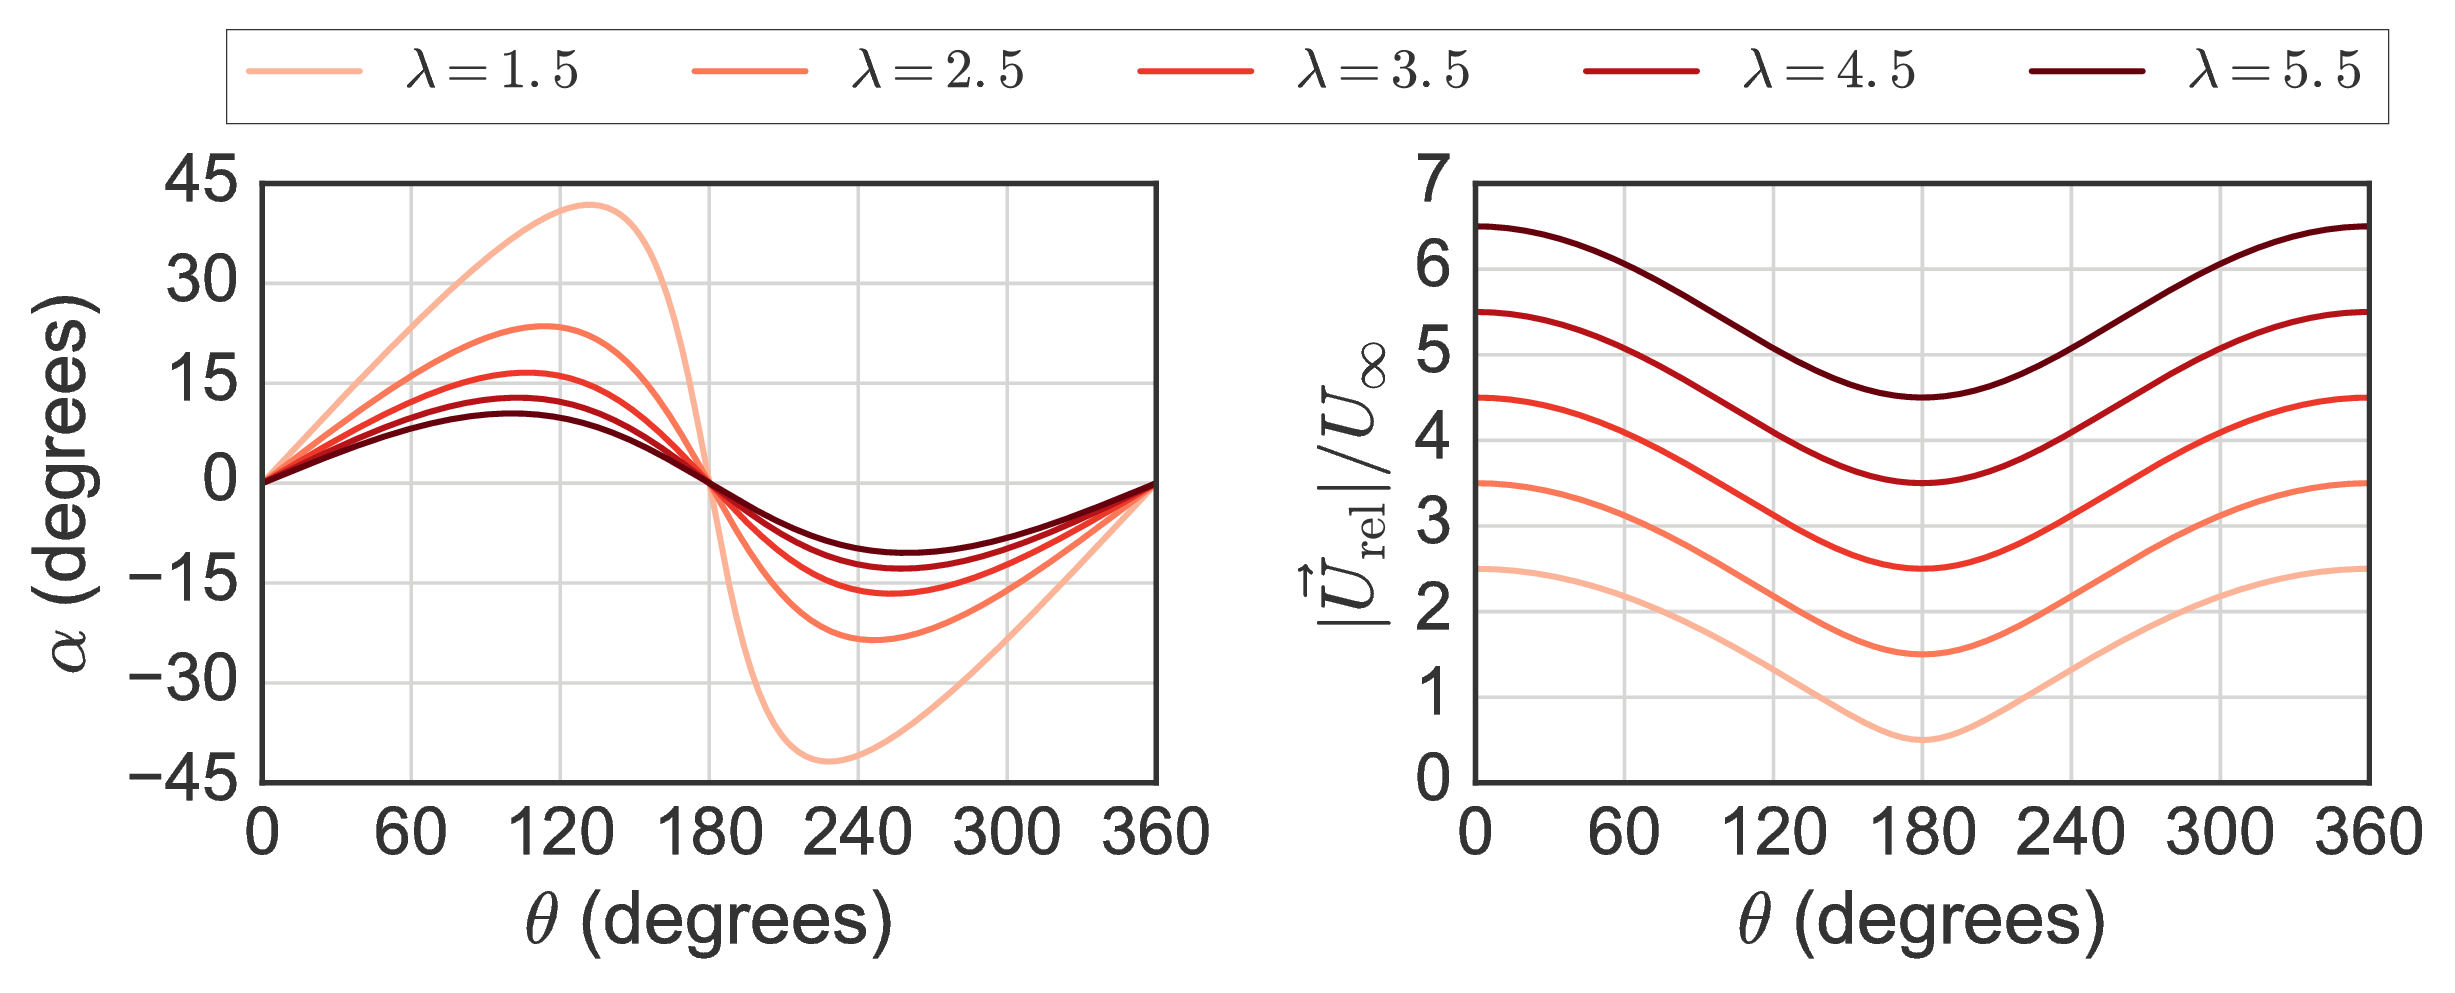
\includegraphics[width=0.85\textwidth]{CFT-vectors_alpha_deg_urel_geom}
    
    \caption{Geometric angle of attack (left) and relative velocity (right)
        versus azimuthal angle at various tip speed ratios.}
    
    \label{fig:geom-alpha-urel}
\end{figure}

As shown in Figure~\ref{fig:vectors}, the blade's lift to drag ratio and angle
of attack can be thought of as the quantities to maximize in order to develop
shaft torque. However, beyond a threshold angle of attack, i.e., the static
stall angle, $C_l/C_d$ drops. Predicting foil characteristics (lift, drag,
pitching moment) is difficult beyond the static stall angle, where boundary
layer separation becomes dominant over most of the foil suction surface, which
reduces lift and increases drag dramatically. For example,
Figure~\ref{fig:S826-perf} shows measured lift and drag coefficients compared
with 2-D and 3-D Navier--Stokes CFD simulations from Cakmakcioglu \etal
\cite{Cakmakcioglu2014}. The linear lift slope region and static stall angle are
predicted well enough, but the peak $C_l/C_d$ is massively overestimated. This
may not be an issue for a machine designed to operate at relatively fixed and/or
pre-stall $\alpha$, e.g., airplane wings, propellers, or axial-flow wind
turbines, but a cross-flow turbine will most likely encounter post-stall
regimes, making even high-fidelity CFD analysis an uncertain prospect for
accurate blade load prediction.

\begin{figure}[ht]
    \centering
    
    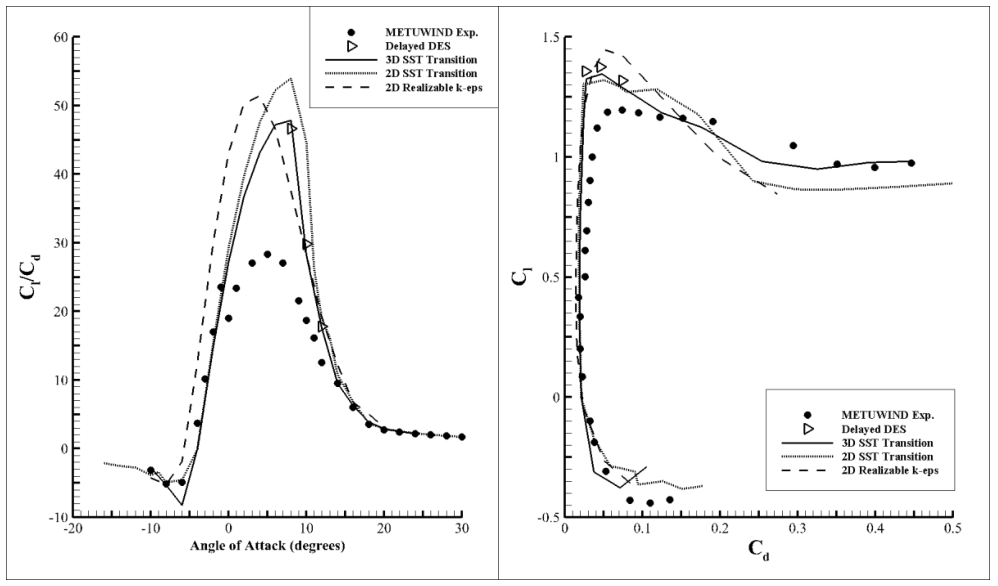
\includegraphics[width=\textwidth]{Cakmak-et-al-2014-fig8}
    
    \caption{Characteristics of an S826 airfoil at $Re=145,000$, from
        \cite{Cakmakcioglu2014}.}
    
    \label{fig:S826-perf}
\end{figure}


\subsection{Unsteady aerodynamics and dynamic stall}

Up until now we have only considered the static behavior of foils, which may be
sufficient to model the steady performance of an axial-flow turbine, since rotor
blade element angles of attack are meant to remain constant in ideal conditions.
The rotation of a cross-flow turbine, however---with its constantly changing
angle of attack (also the change in sign) and relative velocity---produces an
unsteady environment for the blade elements, even in an idealized case.

Unsteady foil behavior had been studied extensively in rotorcraft research. In
the absence of stall, even a helicopter rotor airfoil will deviate from static
behavior due to cyclic pitching, along with changes in relative velocity as the
blade advances and retreats. Thus, the wealth of knowledge available from the
helicopter literature provides insight into the cross-flow turbine case.

The first consideration is the attached behavior of unsteady airfoils. As one
might expect, in these cases either the angle of attack or relative velocity is
varying, but large amounts of flow separation, i.e. stall, is never encountered.
The unsteadiness is characterized by a reduced frequency~\cite{Leishman2006}
\begin{equation}
    k = \frac{\omega c}{2 U_\infty},
\end{equation}
which assumes the free stream velocity is constant. Unsteady effects begin to
become significant for $k > 0.05$, and can become dominant for $k \ge 0.2$.

For a cross-flow turbine reduced frequency can be reformulated in terms of the
tip speed ratio as
\begin{equation}
    k = \frac{\lambda c}{2R}.
\end{equation}
As an example, a large scale, relatively low solidity Darrieus turbine such as
the Sandia 34 m diameter Test Bed, with an equatorial blade chord of 0.91 m
\cite{Murray2011}, a reduced frequency of 0.16 is encountered based solely on
angle of attack oscillations at $\lambda=6$. For a smaller scale CFT, e.g., with
$c/R = 0.25$, operating at $\lambda = 2$, the reduced frequency is 0.25. It
follows that unsteady effects will be significant for cross-flow turbines even
in the absence of nonlinear effects such as stall.

In the unsteady regime, when angle of attack is high enough to induce large
separation it is called dynamic stall. The effects on foil loading are different
from those of static stall in that they are time dependent and include
hysteresis or lag effects. The dynamic stall process in general can be described
as \cite{McCroskey1981}:
\begin{enumerate}
    \item A large leading edge vortex is formed, which causes an overshoot in
    lift beyond the static case in a linear fashion.
    
    \item The vortex is advected downstream, causing additional lift.
    
    \item The vortex reaches the trailing edge and the lift decays rapidly.
    
    \item Lift slowly returns to the linear regime as flow reattaches.
\end{enumerate}

Based on Figure~\ref{fig:geom-alpha-urel}, we expect dynamic stall to play an
important role in governing overall blade loading for a cross-flow turbine.
Therefore, it is necessary to either accurately model dynamic stall, or employ
CFD methods that can resolve unsteady effects in the foil boundary layer, both
of which will be explored in later chapters.


\section{The state of engineering tools for CFTs}

\subsection{For individual devices}

Presently, the most reliable predictor of turbine performance is physical
modeling (building prototypes or copying existing designs that have been
field-tested), so long as important dynamical scales (Reynolds number, mainly)
are sufficiently matched. It has been shown that performance becomes essentially
Reynolds number independent at an approximate blade chord Reynolds number $Re_c
\approx \lambda U_\infty c / \nu = O(10^5)$ \cite{Bravo2007}, which is
investigated further in later chapters. However, experiments at this scale can
be quite expensive. For example, a turbine with a 1 m diameter and 10 cm chord
would need to be tested in a flow on the order of 1 m/s in water and 10 m/s in
air. For a turbine this large it is typically impractical to manufacture many
prototypes to find the optimal design, so numerical modeling is preferred. There
exists a large spectrum of numerical modeling techniques with widely varying
computational cost and fidelity, and sometimes only the most complex and
computationally expensive are trustworthy.

Momentum models are the simplest and cheapest, where the turbine blades are
discretized into blade elements, for which 2-D static lift and drag data are
tabulated. The relative velocity and angle of attack for a blade element are
calculated by seeking a balance between forces computed from the static foil
data and the rate of change of momentum of the fluid passing by the blade
element. Momentum methods break down for large streamwise forces, i.e.,
``induction factors''---common in water and high solidity turbines---and must be
corrected empirically. Despite their deficiencies, these models can do a
reasonable job for low solidity rotors when combined with corrections for
dynamic loading, the most prominent cause of which is dynamic stall
\cite{Para2002}, but fail for high solidity~\cite{Joo2015}. A double multiple
streamtube (DMS) momentum model can compute a full turbine performance curve in
seconds on a modern desktop computer.

Vortex line methods are similar to momentum models, except blade element local
velocity is computed using potential flow theory, where lifting bodies are bound
vortex lines that shed vortex wake elements whose influences are combined via
the Biot--Savart law \cite{Strickland1979}. Sandia National Labs' CACTUS is an
example of a vortex method \cite{Murray2011}. CACTUS has been tested against
experimental data from large, low-solidity wind turbines (those for which
momentum models do well), but has been shown to fail for smaller turbines in
water, which are typically higher solidity \cite{Michelen2014}. Regarding
computing effort, vortex line methods can compute a full turbine performance
curve in minutes---slightly longer than the DMS method, but still quite fast.
The increase in accuracy of the flow field prediction and the robustness with
respect to high turbine loading justify the slightly higher expense of the
vortex line method.

A more sophisticated vortex model is the so-called panel method, where turbine
geometry can be specified arbitrarily as potential flow boundary elements,
negating the need for sectional foil coefficient tables. This is a significantly
more computationally expensive model. A single turbine operating point (not a
full performance curve) computed in three dimensions may take hours on a
conventional desktop PC. Furthermore, boundary layer models are necessary to
predict the occurrence and consequences of dynamic stall \cite{Zanon2012}.

The most computationally expensive models solve the Navier--Stokes equations,
with turbulence modeled with Reynolds-averaging (RANS) or large eddy simulation
(LES)---the former being relatively less expensive, since LES directly solves a
larger portion of the energy spectrum of turbulence. If a body-fitted grid is
used, the actual turbine geometry is included as part of the computational
domain, and the mesh is generally refined next to the solid surfaces to resolve
the boundary layer, i.e., with cells adjacent to walls having a nondimensional
wall distance $y^+ \sim 1$. When only run in two dimensions, RANS methods are
affordable enough to be run on a single CPU, computing a single turbine
operating point in hours. However, 3-D effects are important enough that 2-D
simulations are not reliable, at least as predictors of absolute performance
\cite{Li2013}. 3-D simulations with a body-fitted grid are very expensive
(especially for LES), therefore are practically limited to high performance
computing (HPC) clusters. Even with the high computational expense, these models
are not perfect and results can deviate significantly from experimental
measurements, especially when using RANS models \cite{Li2013}.

Actuator line modeling (ALMs), first used by Sorensen and
Shen~\cite{Sorensen2002}, is a hybrid of the blade element and Navier--Stokes
methods. The turbine is not part of the mesh, but is represented by lines that
move through the flow, acting as momentum sinks, where the resultant force is
computed using 2-D foil data. Negating the needs for a body-fitted grid and
resolving the boundary layer removes a significant amount of computational
effort, but the flow field is still computed more accurately than with momentum
or vortex methods, since nonlinear effects and turbulence are included in the
RANS or LES equations. Removing the need for complex grids is also an advantage
with respect to  mesh generation, which is arguably the largest impediment to
automation in CFD \cite{Slotnick2014}. Computational effort is also
significantly reduced since the ALM does not need a rotating mesh.

To the author's knowledge, at the time of
this writing there has only been one study in the literature investigating the
ALM for CFTs \cite{Shamsoddin2014}, which was performed for a 2-D rotor at very
low Reynolds number, for which performance predictions were not reported.
Assessing its effectiveness is therefore of interest in the present work.


\subsection{For arrays}

Effective turbine array engineering directly depends on accurate prediction of
turbine wake generation, evolution and interaction, along with the impact of
various types of turbulent inflow on power production of each device. Like for
individual turbines, physical modeling is an option for predicting array
performance, though it becomes even more expensive to match relevant dynamical
scales. For this reason, turbine arrays are mainly designed using numerical
methods.

The contemporary industry standard method for predicting array performance
involves the superposition of prescribed wakes \cite{Stevens2014b}. Evolution
can be dependent on a single expansion coefficient chosen by the free stream
turbulence intensity \cite{Jensen1983, Choi2013} or computed by a solution of
the linearized RANS equations with an empirically derived constant eddy
viscosity closure \cite{Ainslie1988}. In light of the CFT's unique near-wake
dynamics, the valitidy of these models is questionable. At the very least they
would need to be recalibrated for CFTs, though their applicability is limited in
the near-wake of any turbine, meaning they are generally inappropriate for
closely-spaced arrays.
	
The next step up in complexity is the actuator disk method, where a constant
body force is added to the Navier--Stokes equations. This method can be
computationally cheap with RANS, or quite expensive and thorough with LES. The
ORPC turbine array is being laid out using the SNL-EFDC code, which uses a
constant uniform force applied to the RANS equations, where the turbine injects
turbulence kinetic energy and dissipation for the model's $k$--$\epsilon$
closure \cite{Nelson2013}. The ability of actuator disk models to predict the
near-wakes of CFTs is of interest in this work.
	
At present simulations with body-fitted grids are limited to one or two turbines
due to computational cost, which means they are impractical for full array
simulations. Thus the actuator line method, when combined with LES, is the most
complex model being used today. The ALM has the benefit of resolving unsteady
flow features created by periodic blade forcing and end effects, ultimately
producing the most accurate parameterization for turbine induced forces in
Navier--Stokes simulations. It has been shown in blind axial-flow turbine
modeling tests that ALM/LES methods fair better when predicting turbine induced
turbulence, and therefore will be more accurate at predicting flow within a
turbine array \cite{Krogstad2013}.


\section{Goals and objectives}

At the most basic level, the goal this research is to work towards the ability
to predict the performance of and flow though an array of cross-flow turbines,
to allow for the evaluation of array layouts, and the prediction of overall
power output and potential environmental effects. The strategy for meeting this
goal includes the following objectives:

\begin{enumerate}
	\item To improve the understanding of both high and low solidity cross-flow
    turbine wakes, most importantly the apparent increased rate of recovery
    compared with axial-flow turbines. This will establish our flow modeling
    targets.
    
    \begin{enumerate}
        \item To evaluate the ability of actuator disk models to predict the
        wakes of cross-flow turbines.
    \end{enumerate}
	
	\item To assess the allowable scale mismatch at which physical models can
	provide results relevant to full-scale devices and arrays.
	
	\item To evaluate the ability of high-fidelity blade-resolved computational
    fluid dynamics and high performance computing to supplement or possibly replace
    experimental work.
    
    \item To investigate actuator line modeling to potentially reduce the
    required computing power necessary for engineering work with CFTs.
\end{enumerate}


\section{Contributions to science and engineering}

Cross-flow turbines are simple machines made from common shapes, but they can
produce very complex flows. Despite their failure in the large scale wind
industry, and beyond their contemporary adoption in marine hydrokinetics, there
is scientific and engineering value to better understanding their behavior. The
flow problem---unsteady foil behavior involving dynamic stall, finite blade span
end effects in curvilinear flows---is complex yet general enough to be
applicable to other unsteady turbomachinery and/or foil flows, e.g., Voith
Schneider propellers, Cyclogyros, or even conventional helicopter rotors.

This work will increase the amount of experimental data available for device
comparison and numerical model validation. This is especially important for CFTs
since typical designs for small wind and MHK use have not yet been established.
This means that in order to be robust, numerical models must be tested against
measurements from turbines with varying design parameters, notably the solidity
and aspect ratio, which affect the unsteadiness and significance of 3-D effects,
respectively. There is a danger that validating against the most ubiquitous
Darrieus turbine experiments may result in models that fail with newer, more
unique designs.

From this work, open datasets have been generated and published. These datasets
will help others evaluate their numerical models, and since their availability
will also include processing code, other researchers may find new knowledge to
glean from them. 

In summary, this research will elucidate the unique wake properties of
cross-flow turbines, establish scaling guidelines for physical modeling, and
inform designers on the trustworthiness of state-of-the-art numerical modeling
techniques.


% Chapter on developing experimental setup
\chapter{Developing an experimental setup for measuring the performance and
near-wake of cross-flow turbines at large laboratory scale}

The first objective was to acquire high-fidelity experimental data to get a
clear picture of what it is we were trying to predict. We were looking to
acquire both performance data (mechanical power, drag force) and velocity data
in the near-wake. To do this, it was necessary to upgrade the UNH tow tank's
linear motion, control, and data acquisition systems, along with the turbine
test bed instrumentation developed in \cite{Bachant2011-MS}.


\section{Modifications to the UNH tow tank}

\begin{table}
\centering
\begin{tabular}{c|c|c}
Spec & Old system & Target \\ 
\hline
Maximum speed & 1.4 m/s  & 3.0 m/s \\ 
Maximum acceleration & 0.1 m/s$^2$ & 2.0 m/s$^2$ \\ 
Control system & Open loop velocity only & Closed loop position \\ 
On-board power & $4\times12$ V batteries & Continuous 120 and 220 VAC \\ 
\end{tabular}
\caption{Specifications summary for existing and upgraded tow tank systems.} 
\label{tab:tow-tank-specs}
\end{table}

\subsection{Linear guides}

The previous linear guide system consisted of a ``master'' guide constructed from
$4 \times 4$ inch fiberglass tubing, and a ``slave'' guide constructed from aluminum angle, on which plastic wheels rode. Over time, the fiberglass tubing had failed structurally and was covered with stainless steel bars fixed with double-sided tape. These bars shifted around considerably during towing and were a source of noise.

A new set of linear guides was designed from 1.25 inch diameter Thomson 440C
stainless steel linear shafts and super self-aligning linear bearings. The
existing carriage was modified to retrofit the linear bearings, and a series of
parts were designed to adapt the stainless shafts to the existing quasi-level
mounting surfaces, which helped keep cost down.

\subsection{Motion and control}

The tow tank's previous motion system consisted of a 10 horsepower AC induction
motor powered by a Yaskawa V7 variable frequency drive. The motor was coupled to
a speed reducing gearbox, on which a pulley was mounted to drive a 0.25 inch
diameter wire rope. It was seen in previous testing that this system had very
low acceleration ($\sim 0.1$ m/s$^2$), which severely reduced steady state
towing durations. The relatively low spring constant of the wire rope tow member
also gave the system a low natural frequency, which resonated due to cross-flow
turbines' cycling forcing. Furthermore, the system was only velocity-controlled,
and in an open-loop manner. This meant positioning was done manually, which took
a skilled operator, and reduced usable tank length further to allow for
coasting to a stop.

These issues were addressed by changing the motor to a permanent magnet servo
motor, sized to tow turbines with 1 m$^2$ frontal area up to 3 m/s, while
accelerating at 2 m/s$^2$. The motor was powered by a Kollmorgen S700 servo
drive, controlled by an ACS NTM EtherCAT master controller, providing closed
loop position (and velocity) control. A series of emergency stop buttons were
installed to dramatically increase the safety of the system.

A steel-reinforced polyurethane timing belt was chosen as the new drive member.
The most robust timing belt profile---an ATL20---was chosen for maximum
stiffness per unit width, increasing the drive member spring constant roughly by a
factor of 7.


%%% From RM2 test plan %%%

Experiments will be performed in the UNH tow/wave tank, a 36 m long facility
with a 3.66 m wide by 2.44 m deep cross-section, capable of tow speeds up to 3
m/s\footnote{Note that though 3 m/s is the technical limit, the practical limit
    for achieving substantial tow durations is approximately 2 m/s.}, pictured in
Figure~\ref{fig:tow-tank}. The turbine will be mounted in a frame built from
NACA 0020 struts, attached to the tow carriage by four linear bearings, which
transfer all streamwise force to a pair of S-beam load cells. The turbine shaft
RPM will be controlled by a servo motor system, which allows prescription of the
turbine tip speed ratio. The load torque will be measured by an inline rotary
torque transducer and a load cell mounted at a fixed distance from the servo
motor, providing a redundant measurement. Turbine shaft angle will be measured
using the servo drive's emulated encoder output, set to $10^5$ counts per
turbine shaft revolution. Carriage speed, and therefore inflow velocity will be
measured using a linear encoder with 10 $\mu$m resolution. All of these
performance-related quantities will be sampled as 2 kHz, while the tow tank's
motion controller will provide redundant measurements of the carriage speed and
turbine angular velocity sampled at 1 kHz. Turbine wake measurements at 1
turbine diameter downstream will be measured with a Nortek Vectrino+ acoustic
Doppler velocimeter, sampling at 200 Hz. A list of the sensors to be used in the
experiment is shown in Table~\ref{tab:sensors}, instrumentation in
Table~\ref{tab:instrumentation}, and a drawing of the experimental setup is
shown in Figure~\ref{fig:exp-setup}.


\begin{figure}[ht!]
    \centering 
%    \includegraphics[clip,trim=0 0.4in 0 0.37in, 
%    width=0.49\textwidth]{Figures/tow_tank_length} 
%    \includegraphics[clip,trim=0.67in 0 0 0, 
%    width=0.49\textwidth]{Figures/test_bed_photo} 
    \caption{Photos of the UNH towing tank and turbine test bed.} 
    \label{fig:tow-tank}
\end{figure}


\begin{table}[ht]
    \centering
    \begin{tabular}{c|c|c|c}
        Measured quantity & Device type & Mfg. \& model & Nominal accuracy \\
        \hline 
        Carriage position & Linear encoder & Renishaw LM15 & 10 $\mu$m/pulse \cite{RenishawLM15}\\
        Turbine angle & Servo encoder output & Kollmorgen AKD & 10$^5$ pulse/rev \cite{KollmorgenAKD}\\
        Turbine torque & Rotary transducer & Interface T8-200 & $\pm$0.5 Nm \cite{InterfaceT8}\\ 
        Turbine torque (2) & Load cell (\& arm) & Sentran ZB3-200 & $\pm$0.2 Nm \cite{SentranZB}\\
        Drag force, left & Load cell & Sentran ZB3-500 & $\pm$0.6 N \cite{SentranZB}\\
        Drag force, right & Load cell & Sentran ZB3-500 & $\pm$0.6 N \cite{SentranZB}\\
        Fluid velocity & ADV & Nortek Vectrino+ & $\pm$0.5\% $\pm$1 mm/s \cite{NortekVectrino}\\
    \end{tabular}
    \caption{Details of the sensors to be used for the experiment. Note that ``(2)''
        denotes a secondary redundant measurement. ``Turbine torque (2)'' nominal
        accuracy estimated by combining load cell accuracy and arm machining tolerances
        ($\pm 1 \times 10^{-4}$ m) as root-sum-square.} \label{tab:sensors}
\end{table}

\begin{table}[ht]
    \centering
    \begin{tabular}{c|c|c}
        Measured quantity & Device type & Mfg. \& model \\
        \hline 
        Carriage position & Differential counter & NI 9411 \\
        Carriage velocity (2) & Motion controller & ACS NTM \\
        Turbine angle & Differential counter & NI 9411 \\
        Turbine RPM (2) & Motion controller & ACS NTM \\
        Turbine torque & Analog voltage input & NI 9405 \\ 
        Turbine torque (2) & Analog bridge input & NI 9237 \\
        Drag force, left & Analog bridge input & NI 9237 \\
        Drag force, right & Analog bridge input & NI 9237 \\
    \end{tabular}
    \caption{Details of the instrumentation to be used for the experiment. Note that
        ``(2)'' denotes a secondary redundant measurement.}
    \label{tab:instrumentation}
\end{table}

\begin{figure}[ht]
    \centering
%    \includegraphics[clip,trim=0.01in 0 0 0, width=0.95\textwidth]{Figures/tank_cross_section}
    \caption{Illustration of the experimental setup.}
    \label{fig:exp-setup}
\end{figure}


\subsection{Calibrations}

Before collecting data, traceable calibration certificates will be obtained for
the Interface T8-200 torque transducer and NI 9405 and NI 9237 modules. The
torque transducer calibration will be used directly in data processing, while
the drag measurement load cells will be calibrated using an additional Sentran
ZB S-beam load cell and indicator, a package which will also have its own
calibration certificate. This load cell will be mounted to a fixture that allows
varying load on each drag load cell---while the linear bearings are
installed---by a lead screw.  The redundant torque measurement load cell/arm
system will be calibrated in a similar fashion using the Sentran load cell and
indicator, by attaching it to a fixture with a distance from the axis of
rotation known to within approximately 0.005 inches.

\subsection{Synchronization of instrumentation subsystems}

The three data acquisition instrumentation subsystems---motion controller, NI
DAQ (performance measurements), and Vectrino+ (wake velocity
measurements)---will begin sampling at precisely the same time each run, after
being triggered by a TTL pulse created by the motion controller. This strategy
retains synchronization for all performance signal samples (tow speed, torque,
drag, angular velocity), ensuring precise calculation of, e.g., power
coefficient. Since there is also synchronization of the initial sample from each
three subsystems, correlation of events in the performance and wake signals is
also possible.

\subsection{Tare drag and torque compensation} 

Tare torque and drag runs will also be performed to measure the shaft bearing
friction torque and turbine mounting frame drag, respectively. These data will
be similar to the turbine performance data, omitting torque measurements for the
tare drag runs and vice versa. Tare drag runs will be performed for each tow
speed in the experiment, for which the mean value is used in data processing.
Tare torque runs will be performed by rotating the turbine shaft (without
blades) in air at constant angular velocity for a specified duration, over the
range of angular velocities used throughout the experiment. Tare torque will
then be fit with a linear regression versus shaft angular velocity, and added to
the measured turbine torque in post-processing.

%%% End section from RM2


\subsection{Data acquisition and on-board accessories}


\section{Upgraded turbine test bed}


\subsection{Wake measurement system}


\subsection{Software}

Software was developed to automate the entire turbine testing process. Dubbed
\textit{TurbineDAQ}, the desktop application was written in Python due to its
reputation as a good ``glue'' language for systems integration. The graphical
user interface (GUI) was built using the PyQt bindings to the Qt framework.
Communication with the tow tank's motion controller, data acquisition system,
and ADV were integrated into a single application. This combined with the
ability to load and automatically execute test matrices in comma-separated value
(CSV) format allowed for experiments consisting of thousands of tows, where the
previous generation could only realistically achieve around 100.


\section{Determining tank settling time}

Sample tows will be done to determine the amount of time taken between runs such
that the tank has settled adequately, i.e., background turbulence and any large
scale mean flows have been dissipated. This will be assessed by towing the
turbine, then allowing the Vectrino to continue recording velocity data,
monitoring the mean and standard deviation of the signals. The settling times
will be stored in the experiment configuration---one value for each tow speed.


\section{Turbine models}

Two physical turbine models were designed and built.

\subsection{UNH-RVAT}

A primary goal for the UNH-RVAT was geometric simplicity, for the sake of
replication in numerical models. The turbine was model constructed from straight
14 cm chord length NACA 0020 extrusions, used for both the blades and struts.
Blades were mounted at mid-chord and mid-span, having a length of 1 m and placed
at 1 m diameter.

% Below from JoT paper

The turbine model was designed to be geometrically simple, in the spirit of, but
not identical to the Sandia/DOE Reference Model 2 (RM2) CFT \cite{Neary2013,
    Barone2011}. Compared to the full-scale Sandia/DOE RM2, it would be
approximately a 1:6 scale model, albeit with higher solidity, or chord-to-radius
ratio. The turbine rotor is $H=1$ m tall, has a $D=1$ m diameter and was
constructed from three NACA 0020 section blades with constant $c=0.14$ m chord
length, mounted at half-chord and half-span with zero preset blade pitch. The
support struts are also NACA 0020 sections with 0.14 m chord length, and these
are fixed to a $0.095$ m diameter shaft. A sketch of the turbine rotor is shown
in Figure~\ref{fig:expsetup} and CAD models are available from
\cite{Bachant2014-RVAT-CAD}.


\subsection{DOE/SNL RM2}

The turbine is to be a 1:6 scale model of the RM2 rotor. Turbine geometry is to
be scaled from the RM2 ``rev 0'' design report \cite{Barone2011}, with the
exception of the shaft diameter, which will be a scaled version of the SAFL RM2
shaft \cite{Hill2014}. The hub design is also similar to the SAFL model, which
may aid in comparison of the results, though this is not a top priority.
Geometric parameters are shown in Table~\ref{tab:turb-geom} and a drawing of the
turbine design is shown in Figure~\ref{fig:RM2-drawing}. The turbine model
components---blades, struts, shaft, and center hub sections---will be fabricated
from 6061-T6 aluminum, which will be hardcoat anodized per MIL-8625-A, type III,
class 2 specifications.

\begin{table}[ht]
    \centering
    \begin{tabular}{l|l|l}
        & Full-scale & Model (1:6) \\
        \hline 
        Diameter (m)   & 6.450 & 1.075 \\ 
        Height (m)     & 4.840 & 0.8067 \\ 
        Blade root chord (m) & 0.4000 & 0.06667 \\ 
        Blade tip chord (m)  & 0.2400 & 0.04000 \\ 
        Blade profile & NACA 0021 & NACA 0021 \\ 
        Blade mount & 1/2 chord & 1/2 chord \\ 
        Blade pitch (deg.) & 0.0 & 0.0 \\ 
        Strut profile & NACA 0021 & NACA 0021 \\ 
        Strut chord (m) & 0.3600 & 0.06000 \\ 
        Shaft diameter (m) & 0.2540 \cite{Beam2011} or 0.4160 \cite{Hill2014} & 0.06350\\ 
    \end{tabular}
    \caption{RM2 turbine geometric parameters.}
    \label{tab:turb-geom}
\end{table}

\begin{figure}[ht]
    \centering
%    \includegraphics[width=0.5\textwidth]{Figures/turbine}
    \caption{Illustration of the UNH RM2 scaled physical model.}
    \label{fig:RM2-drawing}
\end{figure}

% Chapter on RVAT baseline experiments
\chapter{Baseline experimental characterization of a high solidity cross-flow
turbine}

For the higher solidity turbine---the UNH-RVAT---the performance and near-wake
were measured in an initial experiment. The Reynolds number dependence,
described in Chapter~\ref{chap:Re-dep}, was observed in a separate experiment.

In the present study the CFT's near-wake was examined in more detail, providing
insight into the mechanisms that improve CFT wake recovery rates compared with
AFTs or other axisymmetric turbulent wakes, with the ultimate goal that these
mechanisms can be replicated in simpler models for use in simulations of large
turbine arrays, where resolving actual turbine geometry is prohibitively
expensive. The ability of one such model---an actuator disk inside a
Reynolds-Averaged Navier--Stokes (RANS) simulation---to predict those defining
characteristics is also assessed.

The dominant scales within the turbine's near-wake are evaluated for their
relative importance, loosely following the conceptual framework presented in
Chamorro et al. \cite{Chamorro2012b}, where the turbine was treated as an
``active filter.'' However, by extending this concept it should be cautioned
that this filter could also be nonlinear, i.e., the spectral modifications of
the inflow are dependent on the spectral distribution itself, not a
superposition of effects at each individual scale. It is also expected that a
CFT will introduce even stronger large (turbine) scale variance into the flow,
due to its cyclical forcing from oscillatory blade angles of attack and relative
velocity. The experiments presented here were performed in a towing tank,
providing a very low turbulence intensity inflow (at least as low as the
instrumentation noise floor), which provides an excellent baseline case for
spectral content added to the flow by the turbine, without any modulation of a
turbulent inflow spectra.

Previous detailed experimental studies with CFTs were generally limited in terms
of Reynolds number due to small geometric scale. On the other hand, as expected,
large-scale measurements were typically performed with lower resolution
instrumentation, and with less control of inflow conditions
\cite{Vermeulen1979}. Brochier et al.~\cite{Brochier1986} employed laser-Doppler
velocimetry (LDV) to acquire detailed flow measurements of a small-scale,
quasi-2-D CFT in dynamic stall. Their study was similar in scope to the work
presented here, but was conducted at very low Reynolds number---approximately
two orders of magnitude smaller than the study presented in this paper. More
recently, Tescione et al. \cite{Tescione2014} performed a detailed experimental
campaign, using particle image velocimetry to illuminate vortex structures in
the wake, and how these interact with each other. However, the question still
remains as to why the CFT wake would recover more quickly than that of an AFT.
The study reported here also examined the three-dimensionality of the wake, as
turbine ``end effects'' will no doubt affect interaction with the free stream.

To summarize, the goals of this study were:
\begin{enumerate}
    
    \item To identify the essential features of the near-wake of a cross-flow
    turbine from experimental measurements acquired at sufficiently high Reynolds
    number.
    
    \item To assess the relative importance of mean and turbulent dynamics on the
    transport of momentum and kinetic energy in the wake.
    
    \item To compare the measured CFT wake to numerical predictions from a uniform
    actuator disk force parameterization implemented inside a RANS model, and
    identify the simulations shortcomings.
    
\end{enumerate}


\section{Experimental test plan}

All experiments were performed at a tow speed of 1 m/s, resulting in a Reynolds
number based on turbine diameter of $Re_D = U_\infty D /\nu = 1 \times 10^6$, or
an approximate blade chord Reynolds number of $Re_c \approx \lambda U_\infty
c/\nu = 2.7 \times 10^5$ for $\lambda=1.9$, where tip speed ratio $\lambda
\equiv \omega D / (2 U_\infty)$. Note that this Reynolds number is high enough
to be considered operating in a $Re$-independent regime \cite{Bravo2007}
\cite{Bachant2014}, which is important considering the relevance of the data to
characterize full-scale behavior, and subsequent validation of simplified
numerical models.


\section{Results and discussion}

\subsection{Data processing}

Data from each tow were extracted where the quantities of interest---torque,
drag, and velocity---had reached an approximately stationary mean value. The
time series were then trimmed further such that they correspond to an integer
number of turbine blade passages, to minimize bias from periodicity. Wake data
collection runs included 30 blade passages, which corresponds to approximately
16.5 seconds or 3300 velocity samples at each measuring station. Drag from the
mounting structure, a.k.a. tare drag, was measured by towing with the turbine
removed, and then subtracted from the turbine measurements to provide a better
estimate of the overall drag on the turbine rotor and shaft alone. Similarly,
tare torque was measured by driving the turbine support shaft and bearings in
air and regressing these values linearly with respect to shaft angular velocity.
This tare torque was then added to the measured turbine torque in
post-processing to provide a more accurate estimate for the true hydrodynamic
torque.

The tank was seeded with 11 $\mu$m mean diameter hollow glass spheres to achieve
adequate beam correlation and signal-to-noise ratios, and no filtering was used
on the velocity data, i.e., statistics were computed using all raw samples from
the measurement interval. For computing partial derivatives of velocity
quantities, a central difference scheme was employed. For the boundaries of the
measurement plane, an inward-facing second-order scheme was used. The data
processing and plotting code, along with the reduced dataset are available from
\cite{Bachant2014_data}.

\subsection{Turbine performance}

Performance curves showing the overall power and drag coefficients of the
turbine are shown in Figure~\ref{fig-perf}. The drag coefficient monotonically
increases with increasing tip speed ratio over the entire range tested, and the
power coefficient reaches a maximum of 26\% around a tip speed ratio
$\lambda=1.8$--$1.9$, where the drag coefficient is 0.96.  These curves informed
the selection of the tip speed ratio $\lambda = 1.9$ as the operating point for
detailed near-wake characterization. We expect that at this tip speed ratio the
turbine blades will be operating in dynamic stall over a part of the turbine
rotation \cite{Scheurich2011}, reaching maximum angles of attack of
approximately 35 degrees, and that this will be a significant contributor to the
near-wake structure. Note that the maximum power coefficient could likely be
improved with simple geometric modifications, e.g., changing the blade pitch
\cite{Fiedler2009},  but for this study the geometry was meant to be as simple
as possible,  therefore the blade pitch was left at zero.

\begin{figure}
    \centering
%    \includegraphics[width=1.0\textwidth]{Figures/perf}
    \caption{Mean turbine power (left) and drag (right) coefficients plotted
        versus tip speed ratio.}
    \label{fig-perf}
\end{figure}


\subsection{Wake characteristics}

The turbine wake was characterized at one rotor diameter downstream of the
turbine axis. The flow measurements mapped out the upper half of the turbine
wake over 3 m in the spanwise direction (of 3.66 m tank width; cf.
Figures~\ref{fig-expsetup} and~\ref{fig-coord}) at a tip speed ratio
$\lambda=1.9$, chosen to represent a typical turbine operating set point at
maximum $C_P$.

The near-wake structure is described in terms of its mean velocity, streamwise
vorticity, Reynolds stresses, and turbulence kinetic energy. Dominant time
scales are identified and evaluated for their contribution to the turbulent
spectra. Finally, the processes that lead to replenishment of momentum and
energy in the wake are identified, with the goal of explaining the CFT's
relatively fast wake recovery.

\subsubsection{Momentum and vorticity}

The mean velocity measured in the wake at one turbine diameter downstream is
shown in Figure~\ref{fig-meanvel}. The most obvious characteristics are the
asymmetry and three-dimensionality of the flow field. The peak momentum deficit
is shifted towards the right side of the turbine (looking upstream). We can also
see the effects of blade tip vortex shedding, where flow is moving downward and
to the left, creating strong streamwise mean vorticity near the blade tip at
$y/R=-1$, contours for which are shown in  Figure~\ref{fig-xvorticity}. The
asymmetry may explain observations of counter-rotating turbine pairs helping
speed wake recovery \cite{Dabiri2011}.

\begin{figure}
    \centering
%    \includegraphics[clip, trim=0 0.25in 0 0.95in, width=0.8\textwidth]{Figures/meancomboquiv}
    \caption{Mean velocity at $\lambda=1.9$. Vectors are cross-stream and
        vertical velocities; contours are streamwise velocity. View is looking 
        upstream, with the turbine frontal area indicated by the solid gray lines.}
    \label{fig-meanvel}
\end{figure}

The generation of streamwise vorticity with opposing directions highlights once
again the three-dimensionality of the wake of this turbine, and its difference
from an axisymmetric swirling wake such as that of an axial-flow turbine. The
two regions of counter-rotating vorticity act like an asymmetrical doublet,
propelling fluid downward towards the turbine centerline.

Compared with the rotating cylinder wake measurements of Lam \cite{Lam2009}, we
see a similar asymmetry in the mean streamwise velocity. The wake is less
asymmetrical with respect to the wake centerline for the turbine compared to the
rotating cylinder for the same non-dimensional rotation rate, although some of
these differences may be due to the cylinder experiments' lower Reynolds
numbers. Compared with the end effects of a finite cylinder wake
\cite{Sumner2004}, we do see generation of a counter-rotating vortex pair,
though for a non-rotating cylinder these are symmetric, which is not the case
for the turbine wake, where the vortex pair seems to be tilted. The turbine's
wake is also similar to a finite cylinder wake in a sense that there is a mean
downward velocity directly behind the wake generator. These similarities and
differences give some perspective regarding the use of cylinders for turbine
simulators in physical model studies of arrays, which was considered by
\cite{Pierce2013}.

Compared with an axial-flow turbine wake \cite{Cal2010}, and a rotating actuator
disk model \cite{Wu2011}, axisymmetric streamwise vorticity or swirl is not
observed here, which is one of the reasons for the wakes' differing dynamics.
This can be explained as a consequence of the conservation of angular momentum,
where the AFT imparts a streamwise rotation along its axis due to torque
generation, where the CFT imparts a torque that is perpendicular to the flow.
The AFT mean swirl only propels fluid away from its axis, while the CFT induces
mean flow into its momentum deficit region, albeit in a asymmetric fashion.

\begin{figure}
    \centering
%    \includegraphics[clip, trim=0 0.3in 0 0.3in,width=0.8\textwidth]{Figures/xvorticity}
    \caption{Contours of mean streamwise vorticity. Negative values indicate
        clockwise vorticity.}
    \label{fig-xvorticity}
\end{figure}

Reynolds shear stress contours, shown in Figure~\ref{fig-restress}, quantify the
replenishment of mean momentum by turbulent transport. Regions of high
$\overline{u'v'}$ as well as the observed asymmetry correspond to the regions of
high gradients of streamwise velocity, indicating regions of high turbulence
production. Note that Bachant and Wosnik \cite{Bachant2013} also showed how the
mean velocity and Reynolds stress varied with tip speed ratio.

\begin{figure}
    \centering
%    \includegraphics[clip, trim=0 0.3in 0 0.5in, width=0.8\textwidth]{Figures/uvcont}
%    \includegraphics[clip, trim=0 0.3in 0 0.5in, width=0.8\textwidth]{Figures/uwcont}
    \caption{Contours of Reynolds shear stress.}
    \label{fig-restress}
\end{figure}

To quantify the relative importance of mean and turbulent transport processes,
we rearrange the streamwise Reynolds-averaged momentum equation to isolate terms
contributing to its streamwise derivative. Assuming the flow is stationary in
the mean and incompressible, the equation becomes

\begin{equation}
\begin{split}
\frac{\p U}{\p x}  =  
\frac{1}{U} \bigg{[}
& - V\frac{\p U}{\p y}
- W\frac{\p U}{\p z} \\
& -\frac{1}{\rho}\frac{\p P}{\p x} \\
& - \frac{\p}{\p x} \overline{u'u'}
- \frac{\p}{\p y} \overline{u'v'}
- \frac{\p}{\p z} \overline{u'w'} \\
& + \nu\left(\frac{\p^2 U}{\p x^2}
+ \frac{\p^2 U}{\p y^2}
+ \frac{\p^2 U}{\p z^2} \right)
\bigg{]}.
\end{split}
\label{eq-momentum}
\end{equation}

From the experimental measurements, all of the terms on the right hand side were
computed except for the streamwise pressure gradient and the streamwise ($x$)
derivatives of the Reynolds and viscous stresses; the latter two terms are
expected to be small under a thin shear layer assumption. Totals for all these
terms, normalized by $D/U_\infty$ to assess nondimensional mean momentum
recovery per turbine diameter of downstream distance are plotted in
Figure~\ref{fig-mombargraph}. We see that as expected, viscous diffusion is
almost negligible. The two Reynolds stress transport terms are both significant,
but the vertical advection term dominates, and the horizontal advection term
contributes negatively, corresponding to streamlines diverging around the
turbine. The flow essentially behaves like an inviscid three-dimensional,
non-axisymmetric turbulent wake. If we sum all the terms we obtain a total wake
recovery rate at $x/D=1$ of 12\% per turbine diameter, which would be
interesting to compare with an axial-flow turbine in similar conditions.

\begin{figure}
    \centering
%    \includegraphics[clip, trim=0 0.25in 0 0.2in, width=0.8\textwidth]{Figures/mombargraph}
    \caption{Estimates for the contributions to mean streamwise momentum recovery
        in the streamwise direction, multiplied by two (due to assumed symmetry), 
        averaged over the measurement plane, and
        normalized by the average streamwise velocity, freestream velocity, and turbine 
        diameter.}
    \label{fig-mombargraph}
\end{figure}


\subsubsection{Dominant time scales}

Spectral densities were computed using a fast Fourier transform (FFT) based
algorithm, with a Hanning window applied to the time series. Spectral values
were averaged over 4 adjacent frequencies to reduce noise and increase
confidence intervals. Figure~\ref{fig-fcont} shows the peak
frequency---normalized by the turbine angular frequency---of the cross-stream
velocity energy spectra at each measurement point. We can see how unsteadiness
in the flow is induced primarily at the blade passage frequency, or three times
$f_\mathrm{turbine}$. Note that some higher peak frequencies can also be seen in
this plot, out in regions of low turbulence intensity. This is due to both the
noise floor of the ADV and the wakes of the guy wire supports.

Spectral concentration $\Psi$ is quantified by normalizing the peak value of the
spectral density by the total variance of the signal multiplied by the
spectrum's Fourier frequency interval $\Delta f$, i.e.,
\begin{equation}
\Psi \equiv \frac{S_{\max} \Delta f}{\sigma^2},
\label{eq-spec_cont}
\end{equation}
where $\Delta f \equiv 1/(N \Delta t)$, $N$ is the total number of samples, and
$\Delta t$ is the sampling interval. For a pure harmonic $\Psi = 1$, indicating
all variance contained within a single frequency. This metric provides further
characterization of the turbulence in terms of its range of scales, rather than
the overall variance or turbulence intensity.

A plot of this concentration is also shown in Figure~\ref{fig-fcont}, where it
is evident that energy is more concentrated towards the side of the  turbine
where the blades move upstream, likely seeing lower angles of attack, and
therefore boundary layer separation occurring further towards the trailing edge
of the blade. This concentration is indicative of more coherent motion, or
extraction of energy/momentum from the flow without intense separation, whereas
on the opposite side of the turbine, turbulence generated by the dynamic stall
process is increasing the diffusion of shed vorticity. This effect can be
further illustrated looking at sample spectra for turbine torque coefficient and
cross-stream velocity components at two points on opposite sides of the turbine,
shown in Figure~\ref{fig-multispec}, where the cross-stream velocity at the side
of the turbine inducing massive separation shows a smaller peak in its spectrum
at the blade passage frequency.

\begin{figure}[h]
    \centering
%    \includegraphics[clip, trim=0 0.3in 0 0.5in, width=0.8\textwidth]{Figures/fpeak_v}
%    \includegraphics[clip, trim=0 0.3in 0 0.3in, width=0.8\textwidth]{Figures/fstrength_v}
    \caption{Cross-stream velocity energy spectra peak frequency normalized by
        turbine angular frequency (top) and spectral concentration (bottom). Note that white 
        regions have values higher than the maximum value of the color bar, caused by both 
        noise and wakes of the guy wire supports.}
    \label{fig-fcont}
\end{figure}

\begin{figure}[h]
    \centering
%    \includegraphics[width=0.98\textwidth]{Figures/multispec}
    \caption{Spectral density for (a) torque coefficient, (b) cross-stream velocity at
        $y/R = -1$; $z/H = 0.25$, and (c) cross-stream velocity at 
        $y/R = 1.5$; $z/H = 0.25$. Dashed vertical lines indicate $[1, 3, 6, 9]$
        times the turbine rotational frequency and the shaded gray region indicates the 
        95\% confidence interval for a $\chi^2$ variable with 8 degrees of freedom---twice 
        the number of frequencies over which spectral values were averaged to reduce noise.}
    \label{fig-multispec}
\end{figure}


\subsubsection{Kinetic energy}

Contours of turbulence kinetic energy are shown in Figure~\ref{fig-kcont}. The
turbulence kinetic energy is concentrated near the top and left side of the
turbine, as a result of the blade tip and dynamic stall vortex shedding,
respectively. The lower turbulence kinetic energy on the $+y$ side of the
turbine corresponds with the more concentrated spectral energy of velocity
unsteadiness in this area. This can be interpreted as the lift-induced vorticity
being shed with less separation compared to the $-y$ side of the turbine, where
turbulence is being generated and redistributing energy across a larger
bandwidth. This brings up one potential improvement to actuator line models:
Modulating turbulence fields at the occurrence of dynamic stall.

\begin{figure}
    \centering
    %\includegraphics[clip, trim=0 0.25in 0 0.3in, width=0.8\textwidth]
    %{Figures/meankcont}
%    \includegraphics[clip, trim=0 0.25in 0 0.3in, width=0.8\textwidth]{Figures/kcont}
    \caption{Contours of turbulence kinetic energy,
        normalized by the mean freestream kinetic energy.
        Turbine frontal area is indicated by solid black lines.}
    \label{fig-kcont}
\end{figure}

Like the analysis of the mean streamwise momentum, the mechanisms which play the
most important role in mean kinetic energy recovery as the wake evolves in the
streamwise direction are now examined. The transport equation for the kinetic
energy $K$ associated with the mean flow \cite{TennekesAndLumley}, rearranged to
isolate the streamwise recovery can be written as
\begin{equation}
\begin{split}
\frac{\p K}{\p x}
=
\frac{1}{U}
\bigg{[}
& - \underbrace{V \frac{\p K}{\p y}}_{y\text{-adv.}}
- \underbrace{W \frac{\p K}{\p z}}_{z\text{-adv.}}
% Pressure work:
- \frac{1}{\rho}\frac{\p}{\p x_j} P U_i \delta_{ij}
% Work by viscous forces
+ \frac{\p}{\p x_j} 2 \nu U_i S_{ij} % Not sure if that's capital S...
% Turbulent transport of K
- \underbrace{
    \frac{1}{2}\frac{\p}{\p x_j} \overline{u_i' u_j'} U_i
}_{\text{Turb. trans.}} \\
% Production of k
& + 
\underbrace{
    \overline{u_i' u_j'} \frac{\p U_i}{\p x_j}
}_{k\text{-prod.}}
% Mean dissipation? Bar could be removed, or no? -- yes, capital letter, no bar.
- 
\underbrace{
    2 \nu S_{ij}S_{ij}
}_{\text{Mean diss.}}
\bigg{]}.
\label{eq-K_full}
\end{split}
\end{equation}
The terms of interest are labeled---advection in the cross-stream and vertical
directions, energy transport by turbulent fluctuations, production of turbulence
kinetic energy $k$ through mean shear, and the dissipation due to mean viscous
shear forces. For the tensor terms, streamwise derivatives were ommitted, since
the measurements were limited to a single streamwise distance.
Table~\ref{tab-eqs} lists all components kept for the computation of each
transport term.

\begin{table}
    \centering
    \begin{tabular}{c|c}
        Term in Eq.~\ref{eq-K_full} & Implementation \\ 
        \hline  
        $y$-adv. & $-\frac{V}{U}\frac{\p K}{\p y}$ \\ 
        $z$-adv.  & $-\frac{W}{U}\frac{\p K}{\p z}$ \\ 
        Turb. trans. ($y$) & $-\frac{1}{2U} \big{[} \frac{\p }{\p y}\overline{u'v'}U 
        + \frac{\p }{\p y}\overline{v'v'}V + \frac{\p }{\p y}\overline{w'v'}W \big{]} $\\ 
        Turb. trans. ($z$)  & $-\frac{1}{2U} \big{[} \frac{\p }{\p z}\overline{u'w'}U 
        + \frac{\p }{\p z}\overline{v'w'}V + \frac{\p }{\p z}\overline{w'w'}W \big{]} $\\ 
        $k$-prod.  & $\frac{1}{U} \big{[} \overline{u'v'}\frac{\p U}{\p y}
        + \overline{v'v'}\frac{\p V}{\p y} 
        + \overline{w'v'}\frac{\p W}{\p y} $ \\
        & $ + \overline{u'w'}\frac{\p U}{\p z}
        + \overline{v'w'}\frac{\p V}{\p z}
        + \overline{w'w'}\frac{\p W}{\p z}
        \big{]} $ \\ 
        Mean diss.   & $ - \frac{2 \nu}{U} \big{[}
        \big{(} \frac{\p U}{\p y} \big{)}^2
        + \big{(} \frac{\p U}{\p z} \big{)}^2
        + \big{(} \frac{\p V}{\p y} \big{)}^2 $ \\
        & $
        + \big{(} \frac{\p V}{\p z} \big{)}^2
        + \big{(} \frac{\p W}{\p y} \big{)}^2
        + \big{(} \frac{\p W}{\p z} \big{)}^2
        \big{]} $ \\ 
    \end{tabular} 
    \caption{Terms used to compute contributions to mean kinetic energy recovery.}
    \label{tab-eqs}
\end{table}

Figure~\ref{fig-Kturbtrans} shows estimates of mean kinetic energy transport by
turbulent fluctuations. The structure of this plot indicates that the turbulent
fluctuations transport mean kinetic energy inward towards regions of lower mean
momentum and lower mean kinetic energy. The signs of the terms plotted here can
be understood from Figures 6 and 4. Note that despite lower turbulence kinetic
energy on the $+y$ side of the turbine, magnitudes of the turbulent transport
are similar on both.

\begin{figure}
    \centering
%    \includegraphics[clip, trim=0 0.25in 0 0.3in, width=0.8\textwidth]{Figures/Kturbtrans}
    \caption{Contours of estimated mean kinetic energy transport by turbulent
        fluctuations, where streamwise derivatives are omitted.
        Turbine frontal area is indicated by solid black lines.}
    \label{fig-Kturbtrans}
\end{figure}

Contributions to mean kinetic energy recovery from various mechanisms were
averaged over the  measurement plane using the trapezoidal rule. Figure~\ref
{fig-Kbargraph}  shows the normalized sum of each quantity to show their
relative size. As with the momentum, the cross-stream mean advection contributes
negatively since the flow is accelerating around the turbine due to its pressure
disturbance, where streamlines diverge.

Viscous dissipation due to mean shear is essentially negligible compared to
the other terms, which is to be expected in a high Reynolds number shear flow a 
short distance downstream of the shear flow (wake) generator (CFT).

Production of turbulence kinetic energy acts to reduce mean kinetic energy, as
expected for the mean kinetic energy equation. The turbulent transport terms,
separated by the direction of their divergence, i.e., ``$y$-turb.'' is a sum of
all terms with $\p / \p y$ in them and ``$z$-turb.'' is a sum of all terms with
$\p / \p z$ in them, are about the same order of magnitude, both roughly an
order of magnitude smaller than the vertical advection term, which is the
largest. It should be re-stated that the terms in Figure~\ref{fig-Kbargraph}
were evaluated in the near wake, in a measurement plane at $x/D=1$ shown in
Figure~\ref{fig-coord}.

Compared to the observations of Kinzel et al. \cite{Kinzel2012}, where the
turbulent transport terms were found to be not large enough to replenish turbine
power output, it can be seen here that it is most likely vertical advection that
plays the most important role in enhancing the wake recovery, not the turbulence
quantities. This is likely a consequence of the unique vorticity generation and
interaction from lift production, (dynamic) stall vortices, and blade end
effects.

\begin{figure}
    \centering
%    \includegraphics[clip, trim=0 0.25in 0 0.2in, width=0.8\textwidth]{Figures/Kbargraph}
    \caption{Estimates for the contributions to mean kinetic energy recovery
        in the streamwise direction, multiplied by two (due to assumed symmetry), 
        averaged over the measurement plane, and
        normalized by the average streamwise advection velocity, freestream kinetic 
        energy, and turbine diameter.}
    \label{fig-Kbargraph}
\end{figure}


\subsection{Comparison with an actuator disk}

The actuator disk model, commonly used in modern large-eddy simulations of wind
farms \cite{Stevens2014}, parameterizes turbine forcing on the flow field as a
steady streamwise force applied over the frontal area of the turbine. The model
is attractive due to its relatively simple implementation; it does not require
the meshing of actual turbine geometry, making it computationally feasible to
simulate large turbine arrays. For example, the turbine array being installed by
ORPC in Cobscook Bay, Maine was laid out with a RANS actuator disk model, where
cross-flow turbines were represented inside the mesh over three cells
\cite{Nelson2013}. Furthermore, the actuator disk force coefficients are not
time dependent, allowing for simulation of, e.g., tidal cycles without the need
for small time steps to resolve unsteady turbine forcing.

Here the experimental measurements are compared and contrasted with the
near-wake of an actuator disk model, to illustrate how this model would
represent a cross-flow turbine in an array simulation. Since one of the
potential benefits of cross-flow turbines is to be able to be spaced more
closely in an array installation, the near-wake dynamics will be more important
than those of an axial-flow turbine.

For axial-flow turbines, the actuator disk model can be enhanced with a rotating
axial velocity component, which gives better results than a simple volume force
\cite{Wu2011}, but to our knowledge this technique has not been applied
(adapted) to cross-flow turbines. Nevertheless, in the present study the
ability of a simple streamwise force distributed over a cylindrical volume to
mimic the near-wake of a cross-flow turbine was evaluated. As described in
previous sections, the asymmetry of the turbine's wake indicates that a uniform
streamwise force from the actuator disk will likely not capture the wake
accurately.

The open source CFD package \textit{OpenFOAM} was used to solve the  RANS
equations with the turbine represented by an actuator disk, which is
implemented as a force or sink in the momentum equation, applied over a selected
volume of cells in the mesh.

The cross-section of the domain is the same as that of the tow tank used for the
experimental measurements. The actuator disk is technically not a disk, but a 1
m diameter by 1 m tall cylinder, mimicking the turbine swept area. The domain
extends 2 m upstream and 8 m downstream.  The background mesh consists of 96,
64, and 48 points in the $x$, $y$, and $z$ directions, respectively. The cells
in the volume enclosed by the actuator disk region are refined by a factor of
two, giving a total of  approximately $3 \times 10^5$ hexahedral cells. A
snapshot of the mesh is shown in Figure~\ref{fig-AD_mesh}. Boundary conditions
are set to approximate the tow tank environment, i.e., the velocity at the
bottom and walls is set to the free stream value. The free surface was not
modeled---the domain had a rigid lid with a slip velocity boundary condition---a
reasonable approximation for low Froude numbers. Inputs to \textit{OpenFOAM}'s
\texttt{actuationDiskSource} are given in Table~\ref{tab-AS}, and the case files
for this simulation are available from \cite{Bachant2014_OF-AS}.


\begin{figure}
    \centering
%    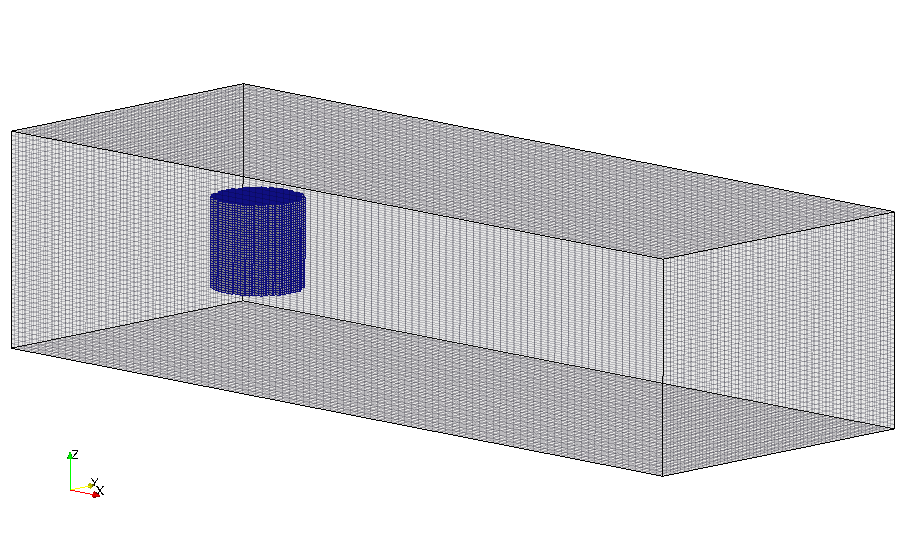
\includegraphics[width=0.9\textwidth]{Figures/AD_mesh}
    \caption{Snapshot of the computational mesh for the actuator disk RANS 
        simulation.}
    \label{fig-AD_mesh}
\end{figure}


\begin{table}
    \begin{center}
        \begin{tabular}{r|l}
            \texttt{Cp} & \texttt{0.26} \\ 
            \texttt{Ct} & \texttt{0.96} \\ 
            \texttt{diskArea} & \texttt{1.0} \\ 
            \texttt{upstreamPoint} & \texttt{(-1.0 0 0)} \\ 
        \end{tabular} 
        \caption{Input parameters for the actuator surface using \textit{OpenFOAM}'s
            \texttt{actuationDiskSource}.}
    \end{center}
    \label{tab-AS}
\end{table}

The turbulence is modeled with a standard $k$-$\epsilon$ closure, with
relatively low levels of inlet turbulence kinetic energy and dissipation, $2
\times 10^{-4}$ and $3 \times 10^{-5}$, respectively. These low free stream
values were chosen to approximate the tow tank ambient conditions.

Results for the mean velocity field are presented in
Figure~\ref{fig-AD_contours}, in a manner similar to that of
Figure~\ref{fig-meanvel}, for comparison. Clearly, the vertical mean flow, which
was determined to be an important driver of near-wake dynamics in the
experiments, is absent. In fact, it contributes negatively to streamwise wake
recovery. This means that all momentum and energy transport back into the
deficit in the wake created by the turbine will need to be facilitated by
turbulent transport (and viscous diffusion, to a much lesser degree). Note also
how acceleration due to blockage is much lower compared to the experiments
despite matching the overall drag coefficient.

Figure~\ref{fig-AD_streamwise} shows the downstream evolution of the centerline
streamwise velocity, and the terms that contribute to its streamwise derivative
averaged over various constant-$x$ planes. Note how very close to the turbine,
the streamwise pressure gradient is contributing significantly to the increase
in $U$, despite the fact that the turbine creates a positive pressure gradient
along the centerline. The large pressure-driven increase in streamwise velocity
makes sense considering the fact that the values are averaged over the entire
cross-section of the domain, which includes a large area of flow acceleration
around the turbine, where the streamwise pressure gradient is negative. Just
after the turbine, $-\p P / \p x$ drops off very quickly and then acts to
decrease streamwise momentum slightly as the static pressure recovers moving
downstream.

We can see that the streamwise momentum recovers very slowly, only starting to
recover around $x=7D$, which can be mostly attributed to the low inflow
turbulence levels, chosen to mimic the tow tank environment. This can be further
understood by looking at the transport terms plotted on the right in
Figure~\ref{fig-AD_streamwise}, where we see all terms are quite small when
compared with the experimental results from the turbine. Rather than the
advection terms, which contribute negatively, the turbulent transport---here
modeled using the $k$--$\epsilon$ eddy viscosity $\nu_t$---is driving the
streamwise evolution, despite being very small. One way to increase the wake
recovery in such a model is to have the actuator disk ``inject'' turbulence
quantities to increase the eddy viscosity \cite{James2011, Nelson2013}. However,
this will likely still not be sufficient to predict evolution and interaction in
closely-spaced arrays of CFTs, since neither the significant vertical mean 
velocities in the CFT wake, nor any coherent vortical structures 
due to blade, shaft, or strut forces are captured by the actuator disk model.

It could be argued that the actuator disk model should not be judged this way as
it is well known that it is a poor predictor of near-wake characteristics,
however, these models are common in engineering practice when calculating
performance of turbine arrays, as previously mentioned. The experiments reported
here have shown that the use of these models would likely be a source of large
uncertainty if applied to cross-flow turbine installations.

\begin{figure}
    \centering
%    \includegraphics[clip, trim=0 0.25in 0 0.5in, width=0.75\textwidth]{Figures/meancomboquiv_AD}
    \caption{Mean velocity predictions at $x/D=1$ from the RANS actuator disk 
        numerical model. Vectors are cross-stream and
        vertical velocities; contours are streamwise velocity.}
    \label{fig-AD_contours}
\end{figure}

\begin{figure}
    \centering 
    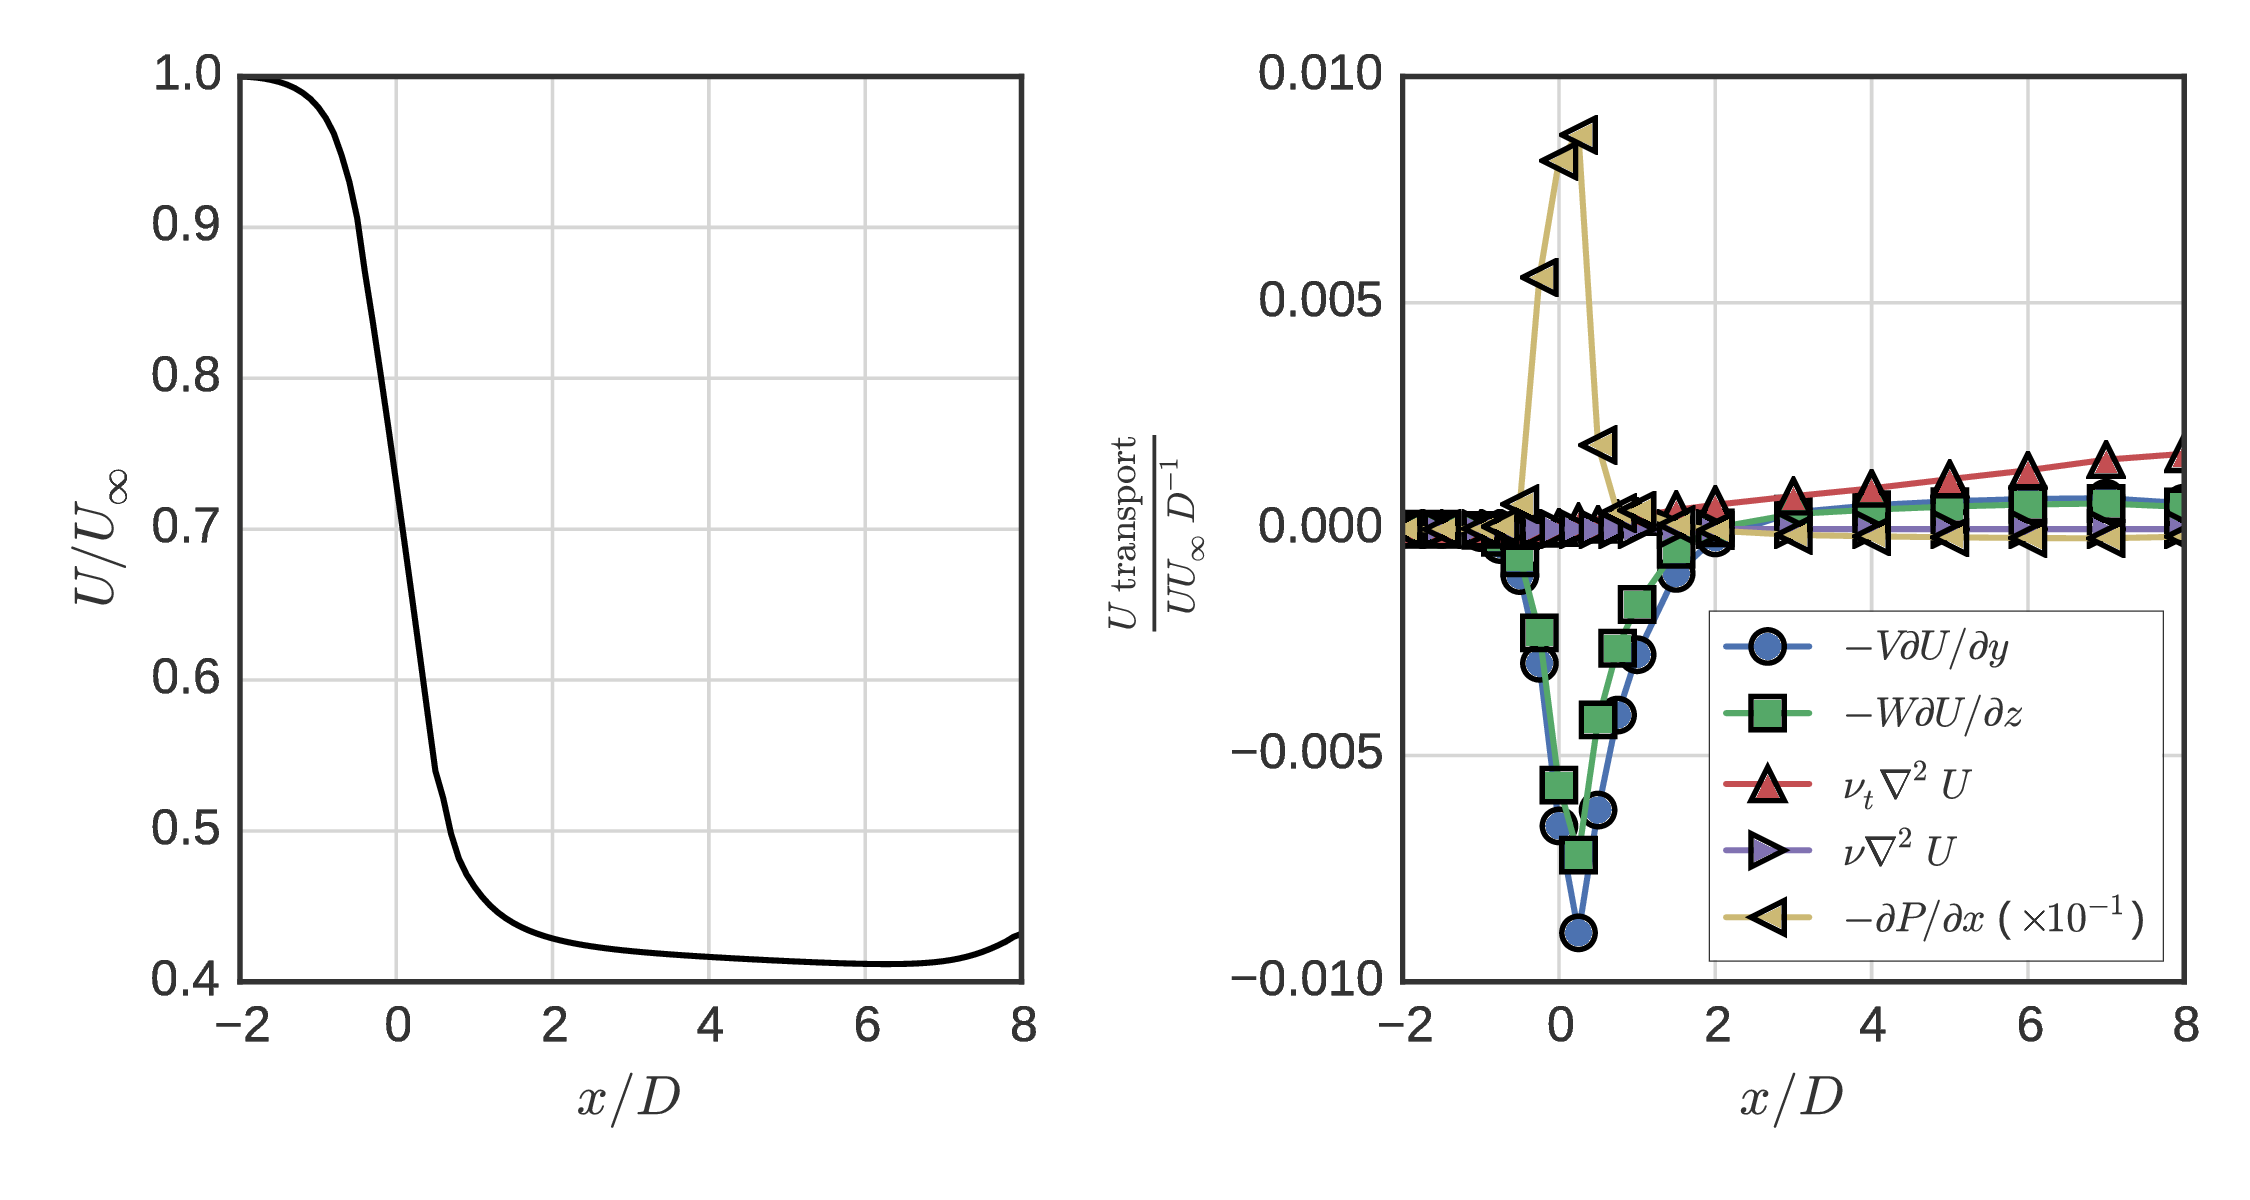
\includegraphics[width=\textwidth]{Figures/AD_streamwise}
    \caption{Downstream evolution of the centerline streamwise velocity (left) and
        normalized momentum transport terms (right) averaged over $y$--$z$ slices from  
        the actuator disk RANS simulation.}
    \label{fig-AD_streamwise}
\end{figure}

\section{Conclusions}

Detailed measurements were performed in the near-wake of a vertical axis
cross-flow turbine operating at peak power coefficient. The following essential
features were identified:

\begin{enumerate}
    \item Asymmetry and three-dimensionality in the mean velocity field. 
    
    \item Mean streamwise swirling flow, or vorticity produced by blade tip and
    dynamic stall vortex shedding, which propels fluid towards the wake's center
    and makes mean vertical advection the largest contributor to streamwise
    momentum and mean kinetic energy recovery.
    
    \item Asymmetric turbulence generation due to the effects of dynamic stall
    being more pronounced on one side of the turbine.
\end{enumerate}

The most dominant timescale induced into the wake is the blade passage period. 
The $+y$ side of the turbine contains more coherent motion at this
frequency, as stalling is less prevalent there. The reduced separation due to 
stall also leads to lower magnitudes of turbulence kinetic energy on the $+y$ 
side. 

Regarding recovery of the mean streamwise momentum and kinetic energy, it was
calculated from the wake velocity measurements that vertical advection is more
than twice as large as transport by turbulent fluctuations, which may explain
why CFT wakes entrain free stream kinetic energy more effectively than their AFT
counterparts. The importance of the vertical flow created by the turbine showed
that array flow simulations will need to be carried out in three dimensions to
produce accurate results. Considering how high power coefficient estimates are
in 2-D simulations \cite{Li2013}, it logically follows that 3-D effects
significantly decrease the power output of a single turbine, but this uncaptured
power helps pull more power from outside the array. This also raises interesting
questions with respect to how cross-flow turbine blades should be
``terminated'', i.e., reducing blade tip vortices by winglets or inhibiting them
with end struts or end disks, as commonly done, may increase the performance of
individual CFTs, however, free ends that produce tip vortices may be
advantageous in an array setting to increase the wake recovery rate.

A commonly used, simple turbine forcing parameterization---an actuator
disk---was assessed for predicting the near-wake characteristics of this turbine
with a RANS simulation. The actuator disk model was found to be a poor
representation of a CFT, despite its computational efficiency and use in
research and industry. It is suggested that an actuator disk with a non-uniform
distribution of force, and an actuator line, may produce the asymmetry and
unsteadiness that is characteristic of the CFT near-wake and will be necessary
to predict performance of closely-spaced arrays that cross-flow turbines are
thought to enable.

% Chapter on Re dep experiments
\chapter{Reynolds number effects on the performance and near-wake of a high
solidity cross-flow turbine} \label{chap:Re-dep}

The use of scaled physical models is common practice in engineering and science
to both assess designs against their requirements and evaluate (validate) the
methods---often computational---use to predict their behavior. Scaling models
helps reduce cost, but relevant physical parameters are then often mismatched.


% Chapter on RM2 experiments, including wake, Re dep, strut drag
\chapter{Experimental characterization of a low-solidity cross-flow turbine}

For the low solidity RM2, the performance was characterized at multiple Reynolds
numbers, with the near-wake at only one, for comparing to the RVAT baseline
data.

\subsection{Turbine model}

The RM2 CFT was initially conceptualized by Sandia National Labs for the US
Department of Energy to be a generic case for numerical modeling
\cite{Barone2011}, specifically Sandia's CACTUS vortex model. With the blade and
strut parameters specified, a turbine model was designed and machined from
6061-T6 aluminum. The hub design mimicked that of the smaller scale RM2 build by
the Saint Anthony Falls Laboratory (SAFL) \cite{Hill2014}, though the blade to
strut connections were more streamlined.

\section{Experimental test plan}

% Chapter on blade-resolved RANS
\chapter{On the use of high-fidelity computational fluid dynamics}

Computing power has reached the level where it is feasible to simulate a
cross-flow turbine by solving the 3-D Reynolds-averaged Navier--Stokes equations
on a boundary layer-resolving body-fitted grid. It is of interest to determine
the accuracy of such a simulation, since as previously discussed the flow
physics of CFTs are very complex.

\section{Comparing cost with physical modeling}


\section{Conclusions}

2-D blade-resolved RANS simulations have been shown to be a poor predictor of
turbine performance.

3-D blade-resolved RANS simulations have been shown to be a fair predictor of
turbine performance and wake characteristics, though the computational cost is
too expensive to be used for engineering work, especially considering the
uncertainty involved compared with physical model studies.

% Chapter on developing ALM and its results
\chapter{Development and evaluation of an actuator line model for cross-flow
    turbines}\label{chap:ALM}

Despite its apparent---but not completely certain---effectiveness for predicting
the performance and wake of a single turbine, blade-resolved CFD presents a huge
computational expense since it must resolve fine details of the blade boundary
layers, and must be performed in three dimensions, which will preclude its use
for array analysis until the availability of computing power increases
sufficiently. It is therefore necessary to explore simpler models that can
predict the turbine loading and flow field with acceptable fidelity, but that
are economical enough to not require high performance computing, at least for
individual devices.

Very fast solution times can be obtained with blade element momentum (BEM)
models, such as the double multiple streamtube (DMST) approached developed by
Paraschivoiu~\cite{Para1988}. However, their poor performance for high solidity
turbines \cite{Joo2015}, makes them less attractive, particular for marine
hydrokinetic applications. Their description of the flow field is very crude as
well, simply computing the momemtum contained within discretized streamtubes,
which cannot resolve any of the complicated flow structures shed by the rotor.

Blade element based vortex line methods can be computationally
feasible---ranging from an expense close to BEM up to that of 2-D blade-resolved
CFD. The cost is a function of the number of vortex elements, which for free
vortex methods increases at each time step, slowing down the calculation as it
marches forward in time. Vortex methods can resolve more flow details than BEM.
However, since the flow is governed by the Laplace equation, nonlinear effects
such as the turbulent transport will not be included, which we have determined
in experiments to be the same order of magnitude as the mean vertical advection.

It is therefore desirable to retain a Navier--Stokes description of the flow
field and use an actuator-type model for parameterizing the turbine loading,
which dramatically drives down computational expense by removing the need for
complicated meshes with many fine cells to resolve the boundary layers near the
blade surfaces. As shown in Chapter~\ref{chap:RVAT-baseline}, the conventional
uniform actuator disk is not a good candidate for a cross-flow turbine wake
generator, never mind the fact that it does not typically compute performance
predictions. There are then two actuator methods that use blade element theory
to compute blade loading and therefore generate a wake that more closely
resembles that of an actual turbine. These are the actuator cylinder or
swept-surface model (ASSM) and the actuator line model (ALM). The ASSM solves
for the average blade loading along its path and applies this as a constant body
force term in the momentum equation. The ALM takes a similar approach but is an
unsteady method, resolving the blade element locations in time.

The ALM, originally developed by Sorensen and Shen \cite{Sorensen2002}, has
become popular for modeling axial-flow or horizontal-axis turbines, and has been
shown in blind tests to be competitive with blade-resolved
CFD~\cite{Krogstad2013, Pierella2014}. The ALM combined with large-eddy
simulation has become the state-of-the-art for modeling entire wind
farms~\cite{Archer2013, Churchfield2012, Sorensen2015, Fleming2013,
    Fleming2014}. Like other blade element techniques, the effectiveness of the ALM
for AFTs is in part due to the quasi-steady nature of the flow in the blade
reference frame, and the relatively rare occurrence of stall.

The ASSM and ALM were implemented to model a very low Reynolds number 2-D
cross-flow turbine experiment in a flume using large-eddy simulation
(LES)~\cite{Shamsoddin2014}. Performance predictions for this case were not
reported, but the ALM was shown to be more effective at postdicting the wake
characteristics measured in the experiments by Brochier \emph{et
    al.}~\cite{Brochier1986}.

It is therefore proposed that an actuator line model may be the optimal
combination of high-fidelity flow modeling that includes performance
predictions, but with reduced computational expense. Here we will develop and
evaluate its effectiveness for cross-flow turbines.


\section{Theory}

The actuator line model is based on the classical blade element theory combined
with a Navier--Stokes description of the flow field. The ALM treats turbine
blades as lines of blade elements, for which 2-D profile lift and drag
coefficients are given. For each blade element, relative flow velocity and angle
of attack are computed by adding the vectors of relative blade motion and the
local fluid velocity. The blade lift and drag forces are calculated as
\begin{equation}
    F_l = \frac{1}{2} \rho A_\mathrm{elem} C_l |\vec{U}_\mathrm{rel}|^2,
\end{equation}
and
\begin{equation}
    F_d = \frac{1}{2} \rho A_\mathrm{elem} C_d |\vec{U}_\mathrm{rel}|^2,
\end{equation}
where $\rho$ is the fluid density, $A_\mathrm{elem}$ is the blade element
planform area (span $\times$ chord), $\vec{U}_\mathrm{rel}$ is the local
relative velocity, and $C_l$ and $C_d$ are the sectional lift and drag
coefficients, chosen from a table per the local angle of attack. The forces are
then projected onto the rotor coordinate system to calculate torque, overall
drag, etc. Forces from the turbine shaft and blade support struts are computed
in a similar way. After the force on the actuator lines from the flow is
computed, it is then added to the Navier--Stokes equations as a body force or
momentum source (per unit density, assuming incompressible flow):
\begin{equation}
    \frac{\mathrm{D} \vec{u}}{\mathrm{D} t} = - \frac{1}{\rho} \nabla p + \nu
    \nabla^2 \vec{u} + F_\mathrm{turbine}.
\end{equation}


\section{Blade element discretization}

In the ALM, a turbine is a collection of actuator lines, which themselves are
collections of actuator line elements (ALEs). The position of each ALE is a
point in space indicating its quarter-chord location. The element is further
defined by its chord direction vector, chord length, span direction vector, span
length, and velocity vector.

An actuator line is created from defined geometry points, between which ALE
parameters are interpolated linearly. This way, an actuator line can be defined
by fewer geometry points than element locations. For example, an AL with
straight planform boundaries---e.g. a straight or tapered wing---only needs two
geometry points to be fully defined. Figure~\ref{fig:AL-geom} shows and example
schematic of a tapered actuator line with three geometry points at the
half-chord locations and six total elements. Note that the middle geometry point
is technically redundant, but is shown for illustrative purposes. For actuator
lines that represent bluff bodies, e.g., shafts, the chord mount offset is set
to 1/4, such that the element location is centered along the line of geometry
points.

\begin{figure}
    \centering
    
    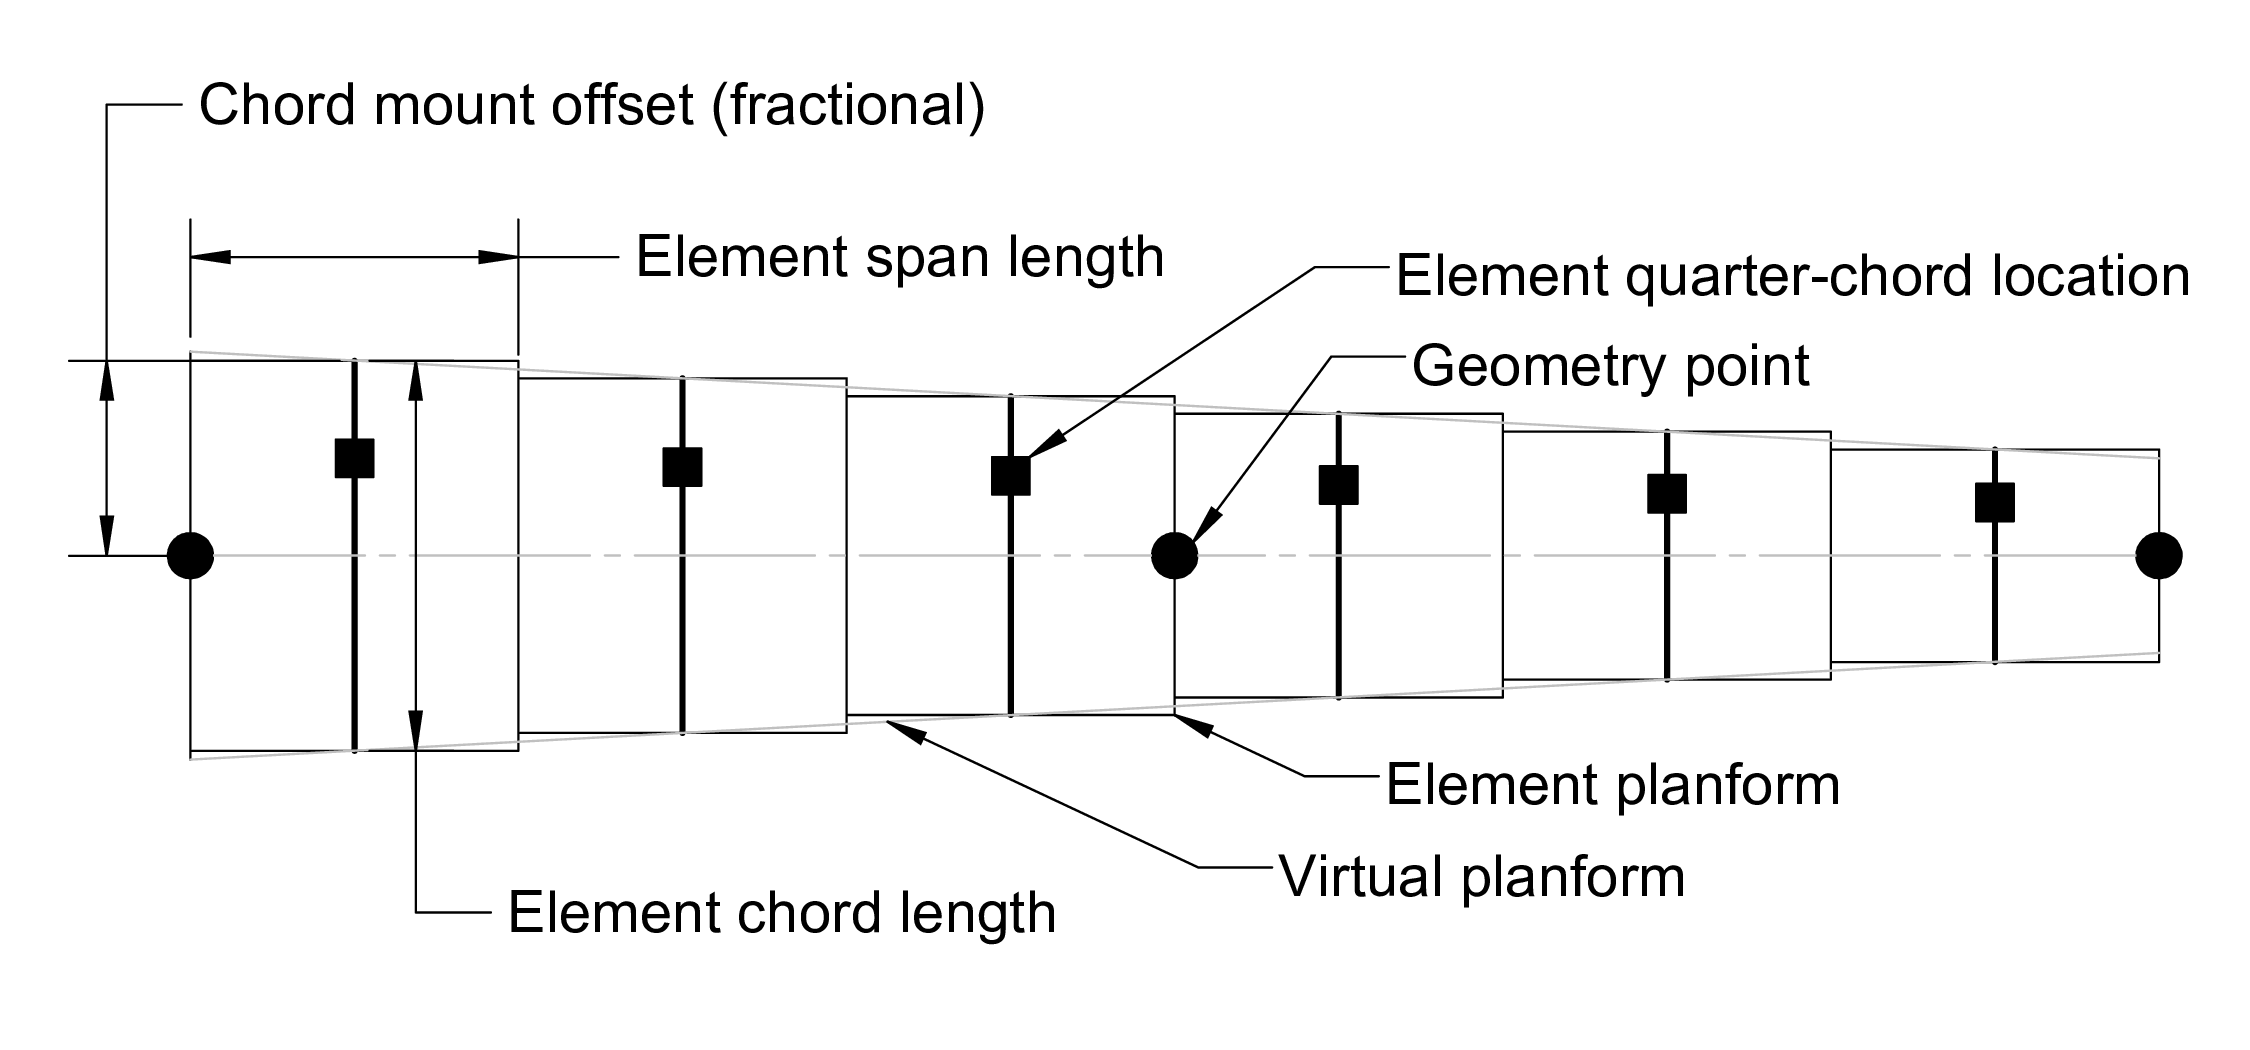
\includegraphics[width=0.9\textwidth]{alm-geometry}
    
    \caption{Actuator line geometry. Filled circles indicate geometry points
        whereas squares indicate actuator line element locations.}
    
    \label{fig:AL-geom}
\end{figure}


\section{Determining inflow velocity}

In momentum methods, the inflow velocity is determined by solving for the axial
and angular induction factors \cite{Manwell2002}. However, using Navier--Stokes
methods, it is somewhat unclear how to calculate the velocity vector used to
compute the angle of attack and relative velocity, though we have access to much
more information about the flow. Sorensen and Shen used an actuator line
element's position to determine the inflow velocity for an axial-flow turbine
\cite{Sorensen2002}. Similarly, Shamsoddin and Porte-Agel use the velocity at a
blade element's location in their actuator line simulation of a vertical-axis
turbine using LES \cite{Shamsoddin2014}. NREL's SOWFA ALM for OpenFOAM also uses
the velocity at the actuator line element location for computing inflow velocity
and local angle of attack with no corrections \cite{Churchfield2013}.

Schito and Zasso developed an effective velocity model (EVM) for computing
actuator forces in Navier--Stokes simulations \cite{Schito2014}. Their EVM
proposes that inflow velocity should be sampled along a line perpendicular to
the mean relative flow direction. They ultimately chose a the line to be 1.5
chord lengths upstream of the actuator point (i.e. quarter-chord location). A
sampling line was chosen to be 5 times the local mesh cell length. Finally, an
angle of attack correction is proposed
\begin{equation}
    \Delta \alpha = \frac{c}{M} (1.2553 - 0.0552 C_d) C_l,
    \label{eq:EVM-dalpha}
\end{equation}
where $c$ is the chord length, $M$ is the mesh size, and $C_l$ and $C_d$ are the
lift and drag coefficients, respectively. Note that the constants in
Equation~\ref{eq:EVM-dalpha} were determined from a calibration with 2-D
blade-resolved CFD for a NACA 0012 foil and are not assumed to be universal.

The EVM, despite showing robustness for its chosen validation case,
unfortunately involves determination of two unknown tuning parameters. To avoid
the additional effort and uncertainty in determining these, the inflow velocity
was sampled at the element quarter-chord location using OpenFOAM's
\texttt{interpolationCellPoint} class, which provides a linear weighted
interpolation using cell values. This algorithm helps keep the sampled velocity
``smooth'' compared with using the cell values themselves, especially when
elements are moving in space as they are in a turbine, since meshes will likely
have a cell size on the same order as the chord length, and will move on the
order of one cell length per time step.


\section{Static foil coefficient data}

Static input foil coefficient data were taken from Sheldahl and
Klimas~\cite{Sheldahl1981}---a popular database developed for CFTs, which
contains values over a wide range of Reynolds numbers. NACA 0021 coefficients
were used for both turbines, despite the fact that the UNH-RVAT is constructed
from NACA 0020 foils, as a NACA 0020 dataset is not available---it is assumed
the small difference in foil thickness is negligible. Since pitching moment data
were only available at limited Reynolds numbers, two datasets were used: The
lowest for $Re_c \leq 3.6 \times 10^5$ and highest $Re_c \geq 6.8 \times 10^5$.
For each actuator line element, blade chord Reynolds number is computed based on
the sampled inflow velocity, and the static coefficients are then interpolated
linearly within the database.


\section{Force projection}

After the force on the ALE from the flow is calculated, it is then projected
back onto the flow field as a source term in the momentum equation. To avoid
instability due to sharp gradients, the source term is tapered from its maximum
value away from the element location by means of a spherical Gaussian function.
The width of this function $\eta$ is controlled by a single parameter
$\epsilon$, which is then multiplied by the actuator line element force and
imparted on a cell with distance $| \vec{r} |$ from the actuator line element
quarter chord location:
\begin{equation}
    \eta = \frac{1}{\epsilon^3 \pi^{3/2}} \exp 
    \left[ - \left( \frac{| \vec{r} |}{\epsilon} \right)^2 \right].
    \label{eq:projection}
\end{equation}

Troldborg~\cite{Troldborg2008} proposed that the Gaussian width should be set to
twice the local cell length $\Delta x$ in order to maintain numerical stability.

Jha \emph{et al.}~\cite{Jha2014} provides guidelines for choosing a projection
width.

Schito and Zasso \cite{Schito2014} found that a projection $\epsilon$ equal to
the local mesh length was optimal.

Martinez-Tossas and Meneveau \cite{Martinez-Tossas2015b} used a 2-D potential
flow analysis to determine that the optimal projection width for a lifting
surface is 14--25\% of the chord length. The width due to the wake caused by the
foil drag force was recommended to be on the order of the momentum thickness
$\theta$, which for a bluff body or foil at large angle of attack is related to
the drag coefficient ($O(1)$) by \cite{TennekesAndLumley}
\begin{equation}
    C_d = 2 \theta / l,
    \label{eq:mom-thickness}
\end{equation}
where $l$ is a reference length, e.g., diameter for a cylinder or chord length
for a foil.

Using these guidelines, three Gaussian width values were determined: one
relative to the chord length, one to the mesh size, and one to the momentum
thickness due to drag force. Each three were computed for all elements at each
time step, and the largest was chosen for the force projection algorithm. Using
this adaptive strategy, fine meshes could benefit from the increased accuracy of
more concentrated momentum sources, and coarse meshes would be protected from
numerical instability.

The Gaussian width due to mesh size $\epsilon_{\mathrm{mesh}}$ was determined
locally on an element-wise basis by estimating the size of the cell containing
the element as
\begin{equation}
    \Delta x \approx \sqrt[3]{V_\mathrm{cell}},
\end{equation}
where $V_\mathrm{cell}$ is the cell volume. To account for the possibility of non-unity aspect ratio cells, an additional factor $C_\mathrm{mesh}$, 2.0 by default, was introduced, giving
\begin{equation}
    \epsilon_{\mathrm{mesh}} = 2C_\mathrm{mesh} \Delta x.
\end{equation}


\section{Unsteady effects}

In the context of a turbine---especially a cross-flow turbine---the actuator
lines will encounter unsteady conditions, both in their angle of attack and
relative velocity. These conditions necessitate the use of unsteady aerodynamic
models to augment the static foil characteristics, both to capture the time
resolved response of the attached flow loading and effects of flow acceleration,
also know as added mass. Furthermore, the angles of attack encountered by a CFT
blade will often be high enough to encounter dynamic stall (DS). It is therefore
necessary to model both unsteady attached and detached flow to obtain accurate
loading predictions.


\subsection{Dynamic stall}

Dynamic stall is encountered when the blade angle of attack changes rapidly in
time and exceeds a certain threshold, often near the static stall angle
\cite{McCroskey1981}. The stall is characterized by an initial increase in lift
beyond static values as a vortex is shed from the foil's leading edge, after
which a drop in lift and large nose-down pitching moment occurs as the vortex is
advected downstream. As the angle of attack drops below the critical value, flow
reattaches, closing the so-called hysteresis loop. Dynamic stall has been shown
to be a significant positive contributor to performance in CFTs \cite{Para2002,
    Urbina2013}, therefore an accurate model is key.

\todo[inline]{Add figure showing dynamic stall cycle.}

DS models were first developed to improve predictive capability for helicopter
rotors, on which DS has significant effects on maneuverability and operational
envelope \cite{Bousman2000}. A summary of dynamic stall models developed for
helicopter rotors is presented in \cite{Leishman2006}. The simplest dynamic
stall models rely on semi-empirical correlations, e.g., the Gormont model
\cite{Gormont1973}, developed at the Boeing--Vertol Company. Several variants of
the Gormont model were developed for vertical-axis wind turbines, with varying
degrees of success; a summary is presented in \cite{Para2002}.

Leishman and Beddoes (LB) developed a semi-empirical model for unsteady
aerodynamics and dynamic stall, which is derived from the phenomenology of the
physics instead rather than pure empiricism \cite{Leishman1989}. Beddoes then
updated the model to the so-called third generation or ``3G'' version
\cite{Beddoes1993}. The LB DS models can be summarized conceptually based on the
following principles:
\begin{itemize}
    \item Dynamic conditions cause a time lag in effective angle of attack and
    lift force.
    
    \item Separation is determined by the Kirchoff flow approximation, which is
    also used to parameterize the normal force coefficient table based on the
    trailing edge separation point. This separation point also encounters a time
    lag.
    
    \item The separation initiates a vortex shedding cycle that causes an
    overshoot and subsequent undershoot in lift before returning to an attached
    flow condition.
\end{itemize}

Sheng et al. \cite{Sheng2008} developed an LB DS model variant targeted at low
Mach numbers. This model, along with the original and 3G LB DS model variants,
was tested for its effectiveness in cross-flow turbine conditions by Dyachuk et
al.~\cite{Dyachuk2014}, who concluded that the Sheng et al. variant results
matched most closely with experiments. In a similar study, the Sheng et al.
model also faired better than the Gormont model \cite{Dyachuk2015}, which
inspired its adoption here for the ALM.

Before the dynamic stall subroutine is executed, the static profile data for
each element is interpolated linearly based on local chord Reynolds number. The
profile data characteristics---static stall angle, zero-lift drag coefficient,
and separation point curve fit parameters---are then recomputed each time step
such that the effects of Reynolds number on the static data are included.

Inside the ALM, angle of attack is sampled from the flow field rather than
calculated based on the geometric angle of attack. Therefore, the implementation
of the LB DS model was such that the equivalent angle of attack
$\alpha_\mathrm{equiv}$ was taken as the sampled rather than the lagged
geometric value. A similar implementation was used by Dyachuk et al.
\cite{Dyachuk2015a} inside a vortex model.


\subsection{Added mass}

A correction for added mass effects, or the effects due to accelerating the
fluid, was taken from Strickland \emph{et al.}~\cite{Strickland1981}, which was
derived by considering a pitching flat plate in potential flow. In the blade
element coordinate system, the normal and chordwise (pointing from trailing to
leading edge, which is opposite the $x$-direction used by Strickland \emph{et
    al.}) coefficients due to added mass are
\begin{equation}
    C_{n_\mathrm{AM}} = -\frac{\pi c \dot{U_n}}{8 | U_\mathrm{rel} |^2}, 
\end{equation}
and
\begin{equation}
    C_{c_\mathrm{AM}} = \frac{\pi c \dot{\alpha} U_n }{8 | U_\mathrm{rel} |^2}, 
\end{equation}
respectively, where $U_n$ is the normal component of the relative velocity, and
dotted variables indicate time derivatives, which were calculated using a simple
first order backward finite difference. Similarly, the quarter-chord moment
coefficient due to added mass was calculated as
\begin{equation}
    C_{m_\mathrm{AM}} = -\frac{C_{n_\mathrm{AM}}}{4} 
        - \frac{U_n U_c}{8 | U_\mathrm{rel} |^2},
\end{equation}
where $U_c$ is the chordwise component of relative velocity. Note that the
direction of positive moment is ``nose-up,'' which is opposite that used by
Strickland \emph{et al.}.

The normal and chordwise added mass coefficients translate to lift and drag
coefficients by
\begin{equation}
    C_{l_\mathrm{AM}} = C_{n_\mathrm{AM}} \cos \alpha + C_{c_\mathrm{AM}} \sin
    \alpha,
\end{equation}
and
\begin{equation}
    C_{d_\mathrm{AM}} = C_{n_\mathrm{AM}} \sin \alpha - C_{c_\mathrm{AM}} \cos
    \alpha,
\end{equation}
respectively. The added mass coefficients were then added to those calculated by
the dynamic stall model.


\section{Flow curvature corrections}

The rotating blades of a cross-flow turbine will have varying angle of attack
along their chords for any given azimuthal location due to the circular
path---producing so-called flow curvature effects~\cite{Migliore1980}. This
makes it difficult to define a single angle of attack for use in the static
coefficient lookup tables. Furthermore, this effect is more pronounced for high
solidity ($c/R$) turbines. Two different flow curvature corrections were
considered; one by Goude \cite{Goude2012} and one by Mandal and Burton
\cite{Mandal1994}.

The Goude correction is derived by considering a flat plat moving along a
circular path in potential flow.

\begin{equation}
    \alpha = \delta + \arctan \frac{V_\mathrm{abs} \cos(\theta_b -
        \beta)}{V_\mathrm{abs} \sin(\theta_b - \beta) + \Omega R} - \frac{\Omega
        x_{0r}c}{V_\mathrm{ref}} - \frac{\Omega c}{4 V_\mathrm{ref}},
    \label{eq:Goude-curvature}
\end{equation}
where $\delta$ is the blade pitch angle, $V_\mathrm{abs}$ is the magnitude of
the local inflow velocity at the blade, $\theta_b$ is the blade azimuthal
position, $\beta$ is the direction of the inflow velocity, $\Omega$ is the
turbine's angular velocity, $R$ is the blade element radius, $x_{0r}$ is a
normalized blade attachment point along the chord, $c$ is the blade chord
length, and $V_\mathrm{ref}$ is the reference flow velocity for calculating
angle of attack.

Note that the code uses vector objects and their associated arithmetic in
software (thanks to OpenFOAM's \texttt{vector} class), which means the first two
terms in Equation~\ref{eq:Goude-curvature} are taken care of automatically given
the inflow velocity, chord direction, and element velocity vectors. Therefore,
the last two terms in Equation~\ref{eq:Goude-curvature} was simply added to the
scalar angle of attack. Note that for a cross-flow turbine, this correction
effectively offsets the angle of attack, which therefore increases its magnitude
on the upstream half of the blade path, and decreases its magnitude on the
downstream half, where the angle of attack is negative.

The Mandal--Burton flow curvature correction assumes that since the blade is
encountering a curvilinear flow, it can be treated as having virtual camber.
They introduce a factor to describe the variation of angle of attack from the
leading to trailing edge
\begin{equation}
    \Delta \alpha = \alpha_\mathrm{TE} - \alpha_\mathrm{LE},
    \label{eq:Mandal-Burton-alpha-diff}
\end{equation}
where TE and LE subscripts denote the values of angle of attack at the trailing
and leading edge, respectively. Calculating these values for an actuator line
element can be done by tracking the leading and trailing edge locations and
velocities, then performing the same vector arithmetic used to calculate the
quarter-chord angle of attack.

An incidence correction factor
\begin{equation}
    \alpha_c = \arctan \left( \frac{1 - \cos (\Delta \alpha / 2)}{\sin (\Delta
        \alpha / 2)} \right)
    \label{eq:Mandal-Burton-alpha-corr}
\end{equation}
is introduced and added to the uncorrected angle of attack. Like the Goude
model, $\alpha_c$ is positive on the upstream half of the turbine rotation and
negative on the downstream half. Both implementations are shown in
Listing~\ref{lst:flow-curvature}.

\begin{lstlisting}[float,caption=Flow curvature model implementation.,label=lst:flow-curvature]
    if (flowCurvatureModelName_ == "Goude")
    {
        angleOfAttackRad += omega_*(chordMount_ - 0.25)
                         * chordLength_/mag(relativeVelocity_);
        angleOfAttackRad += omega_*chordLength_/(4*mag(relativeVelocity_));
    }
    else if (flowCurvatureModelName_ == "MandalBurton")
    {
        // Calculate relative velocity at leading and trailing edge
        vector relativeVelocityLE = inflowVelocity_ - velocityLE_;
        vector relativeVelocityTE = inflowVelocity_ - velocityTE_;
    
        // Calculate vector normal to chord--span plane
        vector planformNormal = -chordDirection_ ^ spanDirection_;
        planformNormal /= mag(planformNormal);
        
        // Calculate angle of attack at leading and trailing edge
        scalar alphaLE = asin((planformNormal & relativeVelocityLE)
                       / (mag(planformNormal)*mag(relativeVelocityLE)));
        scalar alphaTE = asin((planformNormal & relativeVelocityTE)
                       / (mag(planformNormal)*mag(relativeVelocityTE)));
        
        scalar beta = alphaTE - alphaLE;
        
        angleOfAttackRad += atan2((1.0 - cos(beta/2.0)), sin(beta/2.0));
    }
\end{lstlisting}


\section{End effects}

Helmholtz's second vortex theorem states that vortex lines may not end in a
fluid, but must either form closed loops or extend to boundaries. Consequently
the lift distribution due to the bound vortex from foils of finite span must
drop to zero at the tips.

Glauert used Prandtl's lifting line theory to develop a tip loss correction
factor for the blade element analysis of an axial-flow rotor. This was further
developed for horizontal-axis wind turbines by Shen et al. \cite{Shen2005a}.
However, these corrections both depend on the axial-flow rotor tip speed ratio,
number of blades, and tip flow angle, which do not necessarily directly
correspond to cross-flow rotor parameters. Therefore, a more general end effects
model was sought.

From Prandtl's lifting line theory, the geometric angle of attack $\alpha$ of a
foil with an arbitrary circulation distribution can be expressed as a function
of nondimensional span $\theta$ as \cite{Anderson2001}
\begin{equation}
    \alpha (\theta) = \frac{2S}{\pi c (\theta)}
    \sum_1^N A_n \sin \theta
    + \sum_1^N n A_n \frac{\sin n \theta}{\sin \theta}
    + \alpha_{L = 0}(\theta),
    \label{eq:lifting-line}
\end{equation}
where $S$ is the span length, $c(\theta)$ is the chord length, and $N$ is the
number of locations or elements sampled along the foil. This relationship can be
rearranged into a matrix equation to solve for the unknown Fourier coefficients
$A_n$,
\begin{equation}
    [\alpha_m ] - \alpha_{L=0} = [D_{mn}][A_n],
\end{equation}
where
\begin{equation}
    D_{mn} = \sum_1^N \left[ \frac{2b}{\pi c_m} \sin n \theta_m + n \frac{\sin n
        \theta_m}{\sin \theta_m} \right].
\end{equation}

With the Fourier coefficients, the circulation distribution can be calculated as
\begin{equation}
    \Gamma (\theta) = 2SU_\infty \sum_1^N A_n \sin n \theta,
\end{equation}
which, via the Kutta--Joukowski theorem, provides the lift coefficient
distribution
\begin{equation}
    C_l(\theta) = \frac{-\Gamma (\theta)}{\frac{1}{2} c U_\infty}.
\end{equation}

We can therefore compute a correction function 
\begin{equation}
    F = C_l(\theta)/C_l(\theta)_{\max},
\end{equation}
which will be in the range $[0, 1]$, similar to the Glauert corrections, but
does not contain rotor parameters. The correction function for various methods
is compared in Figure~\ref{fig:end-effects}.

\begin{figure}
    \centering
    
    \caption{End effect correction function values for the Glauert, Shen et al.,
        and lifting line methods.}
    
    \label{fig:end-effects}
\end{figure}


\section{Software implementation}

The USA National Renewable Energy Laboratory (NREL) has developed and released
an actuator line modeling library, SOFWA~\cite{Churchfield2014b}, for simulating
horizontal-axis wind turbine arrays using the OpenFOAM finite volume CFD
library. OpenFOAM is free, open-source, and widely used throughout industry and
academia. Though SOWFA is also open-source, its procedural style would have
required significant effort and duplicate code to adapt for cross-flow turbines.
Thus, a new and more general ALM library was developed from the ground up that
could model both cross- and axial-flow turbines, as well as standalone actuator
lines. The actuator line model developed here, dubbed \textit{turbinesFoam}, was
also written as an extension library for OpenFOAM, and was developed freely and
openly from the start in order to increase community engagement and research
efficiency.

\textit{turbinesFoam} was written in OpenFOAM's style, using OpenFOAM's
\texttt{fvOptions} framework for adding source terms to equations at
runtime---see Listing~\ref{lst:fvOptions} for an example implementation within
the Navier--Stokes' momentum equation. Using the \texttt{fvOptions} framework
allows the CFT-ALM to be added to many of the solvers included in OpenFOAM,
meaning it can be readily used with RANS or LES, multiphase models (e.g., for
simulating the free surface in MHK installations), and even with heat transfer.
This is in contrast to SOWFA's implementation, which requires custom flow
solvers to be developed and maintained.

\begin{lstlisting}[float,caption=Adding source terms to the momentum equation in OpenFOAM.,label=lst:fvOptions]
    tmp<fvVectorMatrix> UEqn
    (
        fvm::ddt(U)
        + fvm::div(phi, U)
        + turbulence->divDevReff(U)
        ==
        fvOptions(U)
    );
\end{lstlisting}

OpenFOAM and \textit{turbinesFoam} are written in the C++ programming language,
which follows the object oriented programming paradigm. This characteristic
helped modularize the ALM code for increased readability and reuse. In
\textit{turbinesFoam}, a turbine is a software object that is composed of
actuator line objects, which themselves are composed of actuator line element
objects. Structuring the code this way allows isolation and reuse of the
functionality of individual components. For example, the actuator line object
was written such that is could be used outside the turbine context to ensure is
produces the correct forcing, without adding the complexity of rotation, other
actuator lines, etc. that would be present in a turbine rotor. The very same
actuator line objects can be used in both axial-flow and cross-flow rotors,
without having to copy code from one to the other. In contrast, the actuator
line model in \textit{SOWFA} uses a single software object to represent an
entire array of turbines, which necessitates iterating through many nested lists
down to the element level, which can be confusing to read.

OpenFOAM's data structures are designed to be inherently parallel via message
passing interface (MPI). By working within the library infrastructure the ALM
code was easily parallelized, which will facilitate its deployment on high
performance computing clusters for large flow simulations.

Since all applications are run from a command line and all input data is text
based, automation and integration with other tools is relatively
straightforward. Future enhancements could include coupling with software for
generating static foil data, e.g., XFOIL or other OpenFOAM solvers, turbine
controller models, structural analysis codes, and optimization tools, e.g.,
SNL's DAKOTA \todo[inline]{Get citation for DAKOTA.}, for both individual
turbines and array layouts.


\section{Results}

Both the high solidity UNH-RVAT and low to medium solidity RM2 turbines were
simulated using a $k$--$\epsilon$ Reynolds-averaged Navier--Stokes (RANS)
turbulence model. These rotors provide diverse parameters, which helped evaluate
the robustness of the ALM. The simulations were performed inside a domain
similar in size to that used in Chapter~\ref{chap:CFD}, with similar boundary
conditions. A slice of the mesh in the $x$--$y$ plane is shown in
Figure~\ref{fig:ALM-mesh}.

\begin{figure}
    
    \caption{$x$--$y$ planar slice of the mesh used for the ALM RANS
        simulations.}
    
    \label{fig:ALM-mesh}
\end{figure}

Similar numerical settings were used for each turbine as well. The Sheng et al.
DS model was used with the default coefficients given in \cite{Sheng2008}, and
the Goude flow curvature correction was employed. A second order backward
difference was used for advancing the simulation in time, and second order
linear schemes were used for the majority of the terms' spatial discretizations.
The only major difference between the two simulation configurations was that the
end effects model was deactivated for the RM2, since it reduced $C_P$ far below
the experimental measurements. This modification is at least consistent with the
RM2 blades' higher aspect ratio and tapered planform. Case files for the
UNH-RVAT and RM2 ALM simulations are available from XXX and XXX, respectively.
\todo[inline]{Cite ALM case files.}

The same foil coefficient data were used for all simulations---those for a NACA
0021 as reported by Sheldahl and Klimas \cite{Sheldahl1981}. Each rotor's shaft
was assumed to have a drag coefficient $C_d = 1.1$, and the blade support strut
end element drag coefficients were set to 0.05, to approximate the effects of
separation in the corners of the blade--strut connections.

Since the ALM is intended to be an engineering tool when coupled with RANS, it
was assumed that information about tip speed ratio due to control details would
not be known a priori, and was excluded, unlike the 3-D blade-resolved cases in
Chapter~\ref{chap:CFD}. Note that a systematic investigation of the effects of
sinusoidal $\lambda$ was not undertaken, but for the UNH-RVAT a one to two
percentage point increase in $C_P$ was observed when running with similar
parameters as the blade-resolved simulation.

To evaluate the ALM's ability to predict wake characteristics in a high fidelity
simulation, the UNH-RVAT was also modeled using the Smagorinsky large-eddy
simulation (LES) turbulence model \cite{Smagorinsky1963} in a domain that was
extended slightly to allow for further wake development. Spatial and temporal
grid resolution modifications are discussed below.


\subsection{Verification}

Verification for sensitivity to spatial and temporal grid resolution was
performed for both the UNH-RVAT and RM2 RANS cases, the results from which are
plotted in Figure~\ref{fig:RVAT-ALM-verification} and
Figure~\ref{fig:RM2-ALM-verification}, respectively. Both models displayed low
sensitivity to the number of time steps per revolution. Spatial grid dependence,
however, was more dramatic.

\todo[inline]{Make quantitative statements about verification studies.}

\begin{figure}
    \centering
    
    \caption{Temporal (left) and spatial (right) grid resolution sensitivity
        results for the UNH-RVAT ALM RANS model.}
    
    \label{fig:RVAT-ALM-verification}
\end{figure}

\begin{figure}
    \centering
    
    \caption{Temporal (left) and spatial (right) grid resolution sensitivity
        results for the RM2 ALM RANS model.}
    
    \label{fig:RM2-ALM-verification}
\end{figure}


\subsection{UNH-RVAT RANS}

Power and drag coefficient curves are plotted for the UNH-RVAT in
Figure~\ref{fig:RVAT-ALM-perf-curves}. The ALM was successful at predicting the
performance tip speed ratios up to $\lambda_0$, which suggests that dynamic
stall was being modeled accurately, but $C_P$ was overpredicted at high
$\lambda$. This may have been caused by the omission of additional parasitic
drag sources such as exposed bolt heads and other imperfections located far
enough from the axis to have a large effect at high rotation rates. In
Chapter~\ref{chap:RM2} we showed how these losses can be significant even with
carefully smoothed struts and strut-blade connections. Overprediction of
performance at high tip speed ratio could also be a consequence of the
Leishman--Beddoes dynamic stall model, which can also be seen in the Darrieus
VAWT momentum model results shown in Figure 6.70 of \cite{Para2002}.

\begin{figure}
    \centering
    
    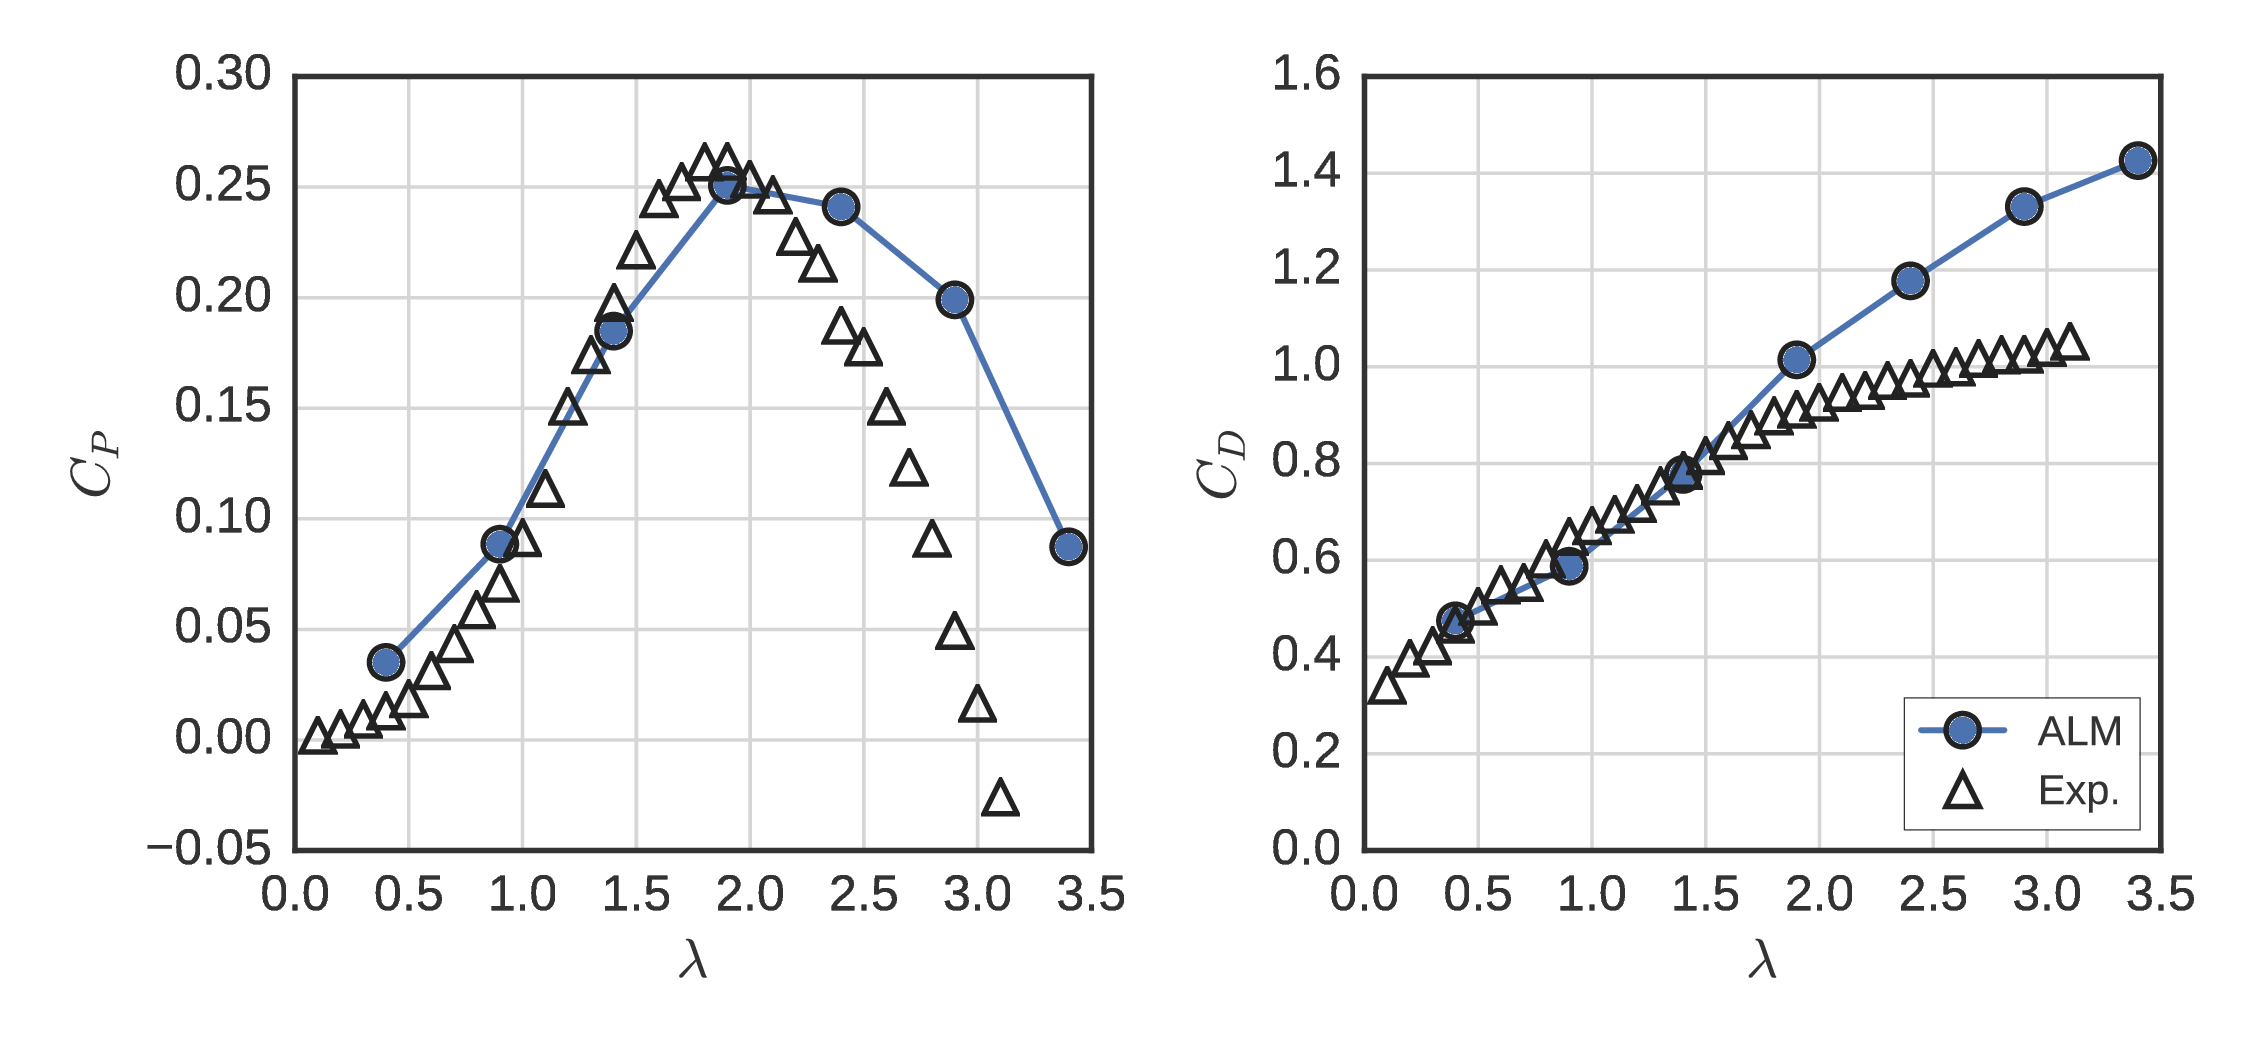
\includegraphics[width=0.85\textwidth]{RVAT-ALM_perf-curves}
    
    \caption{Power and drag coefficient curves computed for the UNH-RVAT using
        the actuator line model with RANS.}
    
    \label{fig:RVAT-ALM-perf-curves}
\end{figure}

Figure~\ref{fig:RVAT-ALM-meancontquiv} shows mean velocity field for the
UNH-RVAT computed by the ALM RANS model. The assymetry was captured well, along
with some of the vertical flow due to blade tip vortex shedding, though the flow
structure is missing the detail present in the experiments and blade-resolved
RANS simulations. Overall, the wake appears to be over-diffused, which could be
a consequence of the relatively coarse mesh. Note that with the DS and flow
curvature corrections turned off, the direction of the mean swirling motion
reverses, which highlights the importance of resolving the correct azimuthal
location of blade loading.

\begin{figure}
    \centering

    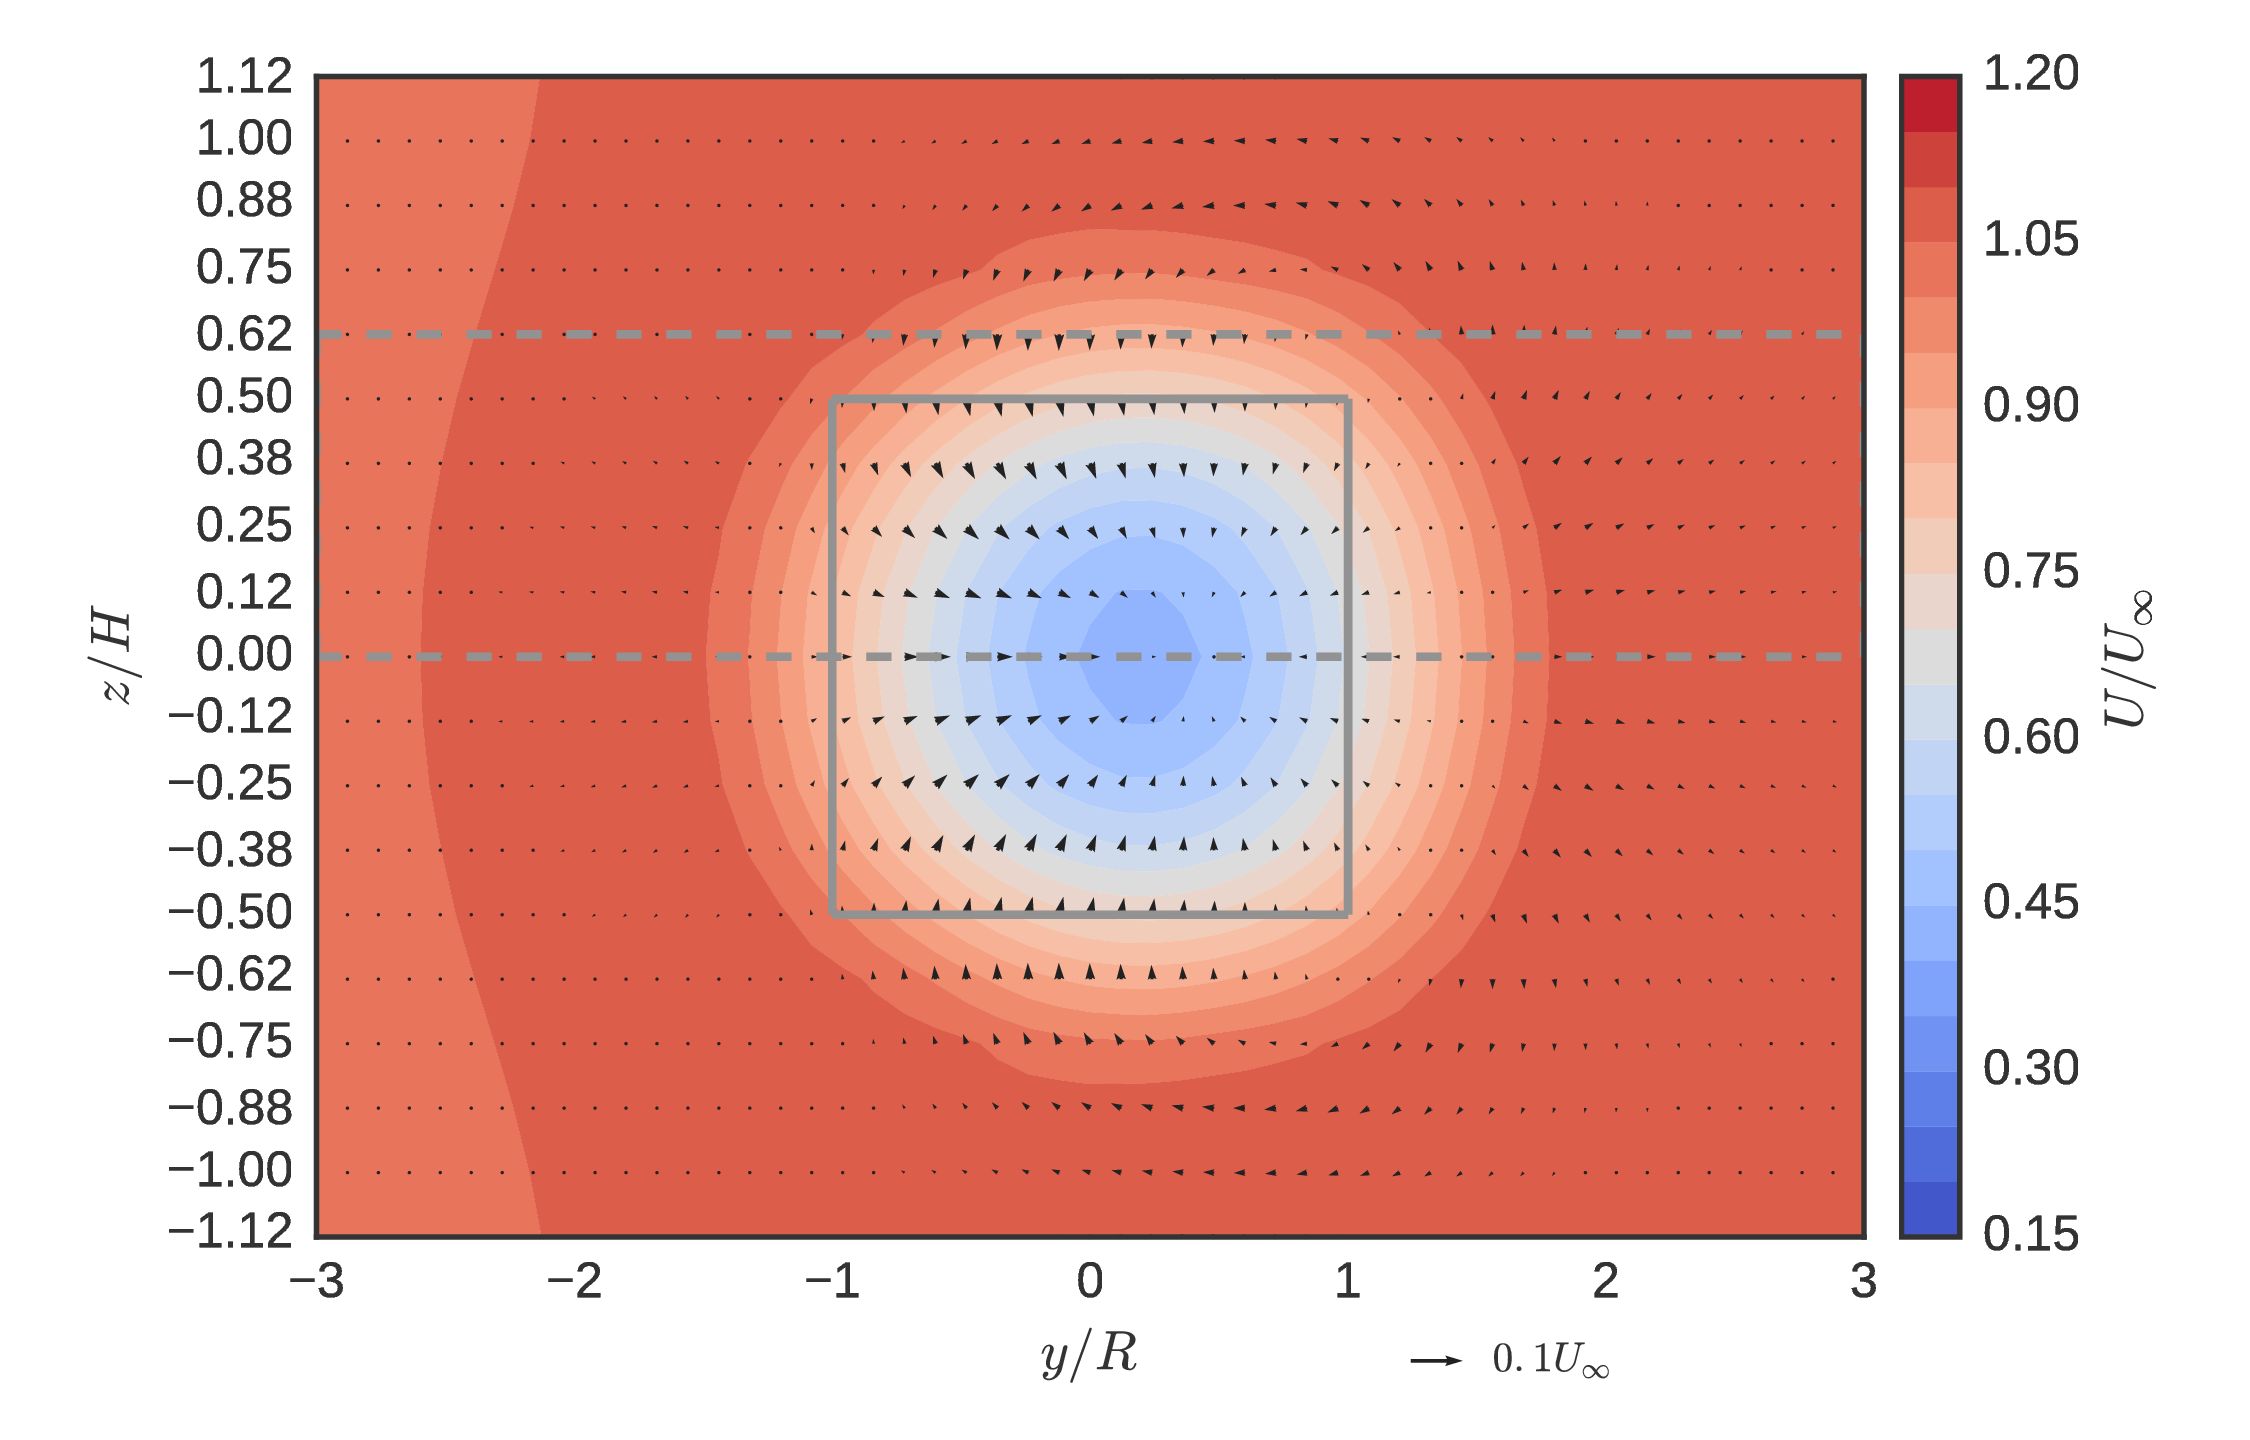
\includegraphics[width=0.9\textwidth]{RVAT-ALM_meancontquiv}
    
    \caption{Mean velocity field at $x/D=1$ with the LB-SGC model, with and
        without the Goude flow curvature correction.}
    
    \label{fig:RVAT-ALM-meancontquiv}
\end{figure}

Turbulence kinetic energy contours (including resolved and modeled energy) are
shown in Figure~\ref{fig:RVAT-ALM-kcont}. The ALM was able to resolve the
concentrated area of $k$ on the $+y$ side of the turbine, but the turbulence
generated by the dynamic stall vortex shedding process is absent. This makes
sense since in the ALM, the DS model only modulates the body force term in the
momentum equation, which does not provide a mechanism for mimicking shed
vortices or turbulence.

\begin{figure}
    \centering

    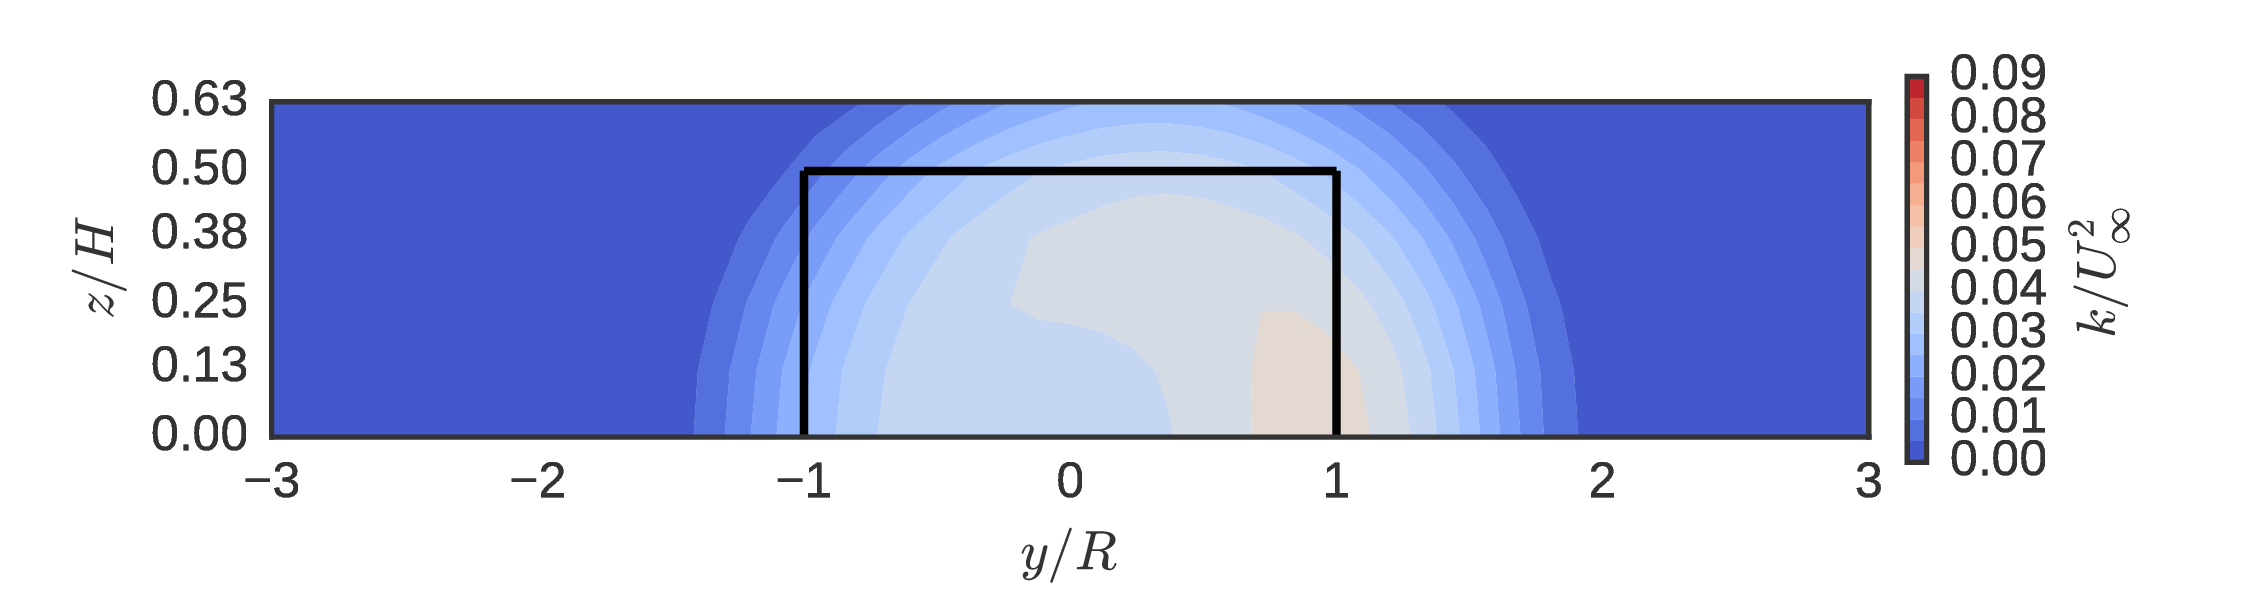
\includegraphics[width=0.85\textwidth]{RVAT-ALM_kcont}
    
    \caption{Turbulence kinetic energy contours at $x/D=1$ predicted by the
        ALM.}
    
    \label{fig:RVAT-ALM-kcont}
\end{figure}

Profiles of mean streamwise velocity and turbulence kinetic energy are shown in
Figure~\ref{fig:RVAT-ALM-profiles}. Here the over-diffused or over-recovered
characteristic of the mean velocity deficit seen in
Figure~\ref{fig:RVAT-ALM-meancontquiv} is more apparent. This effect is also
seen in the profile of $k$, where energy is smeared over the center region of
the rotor.

\begin{figure}
    \centering
    
    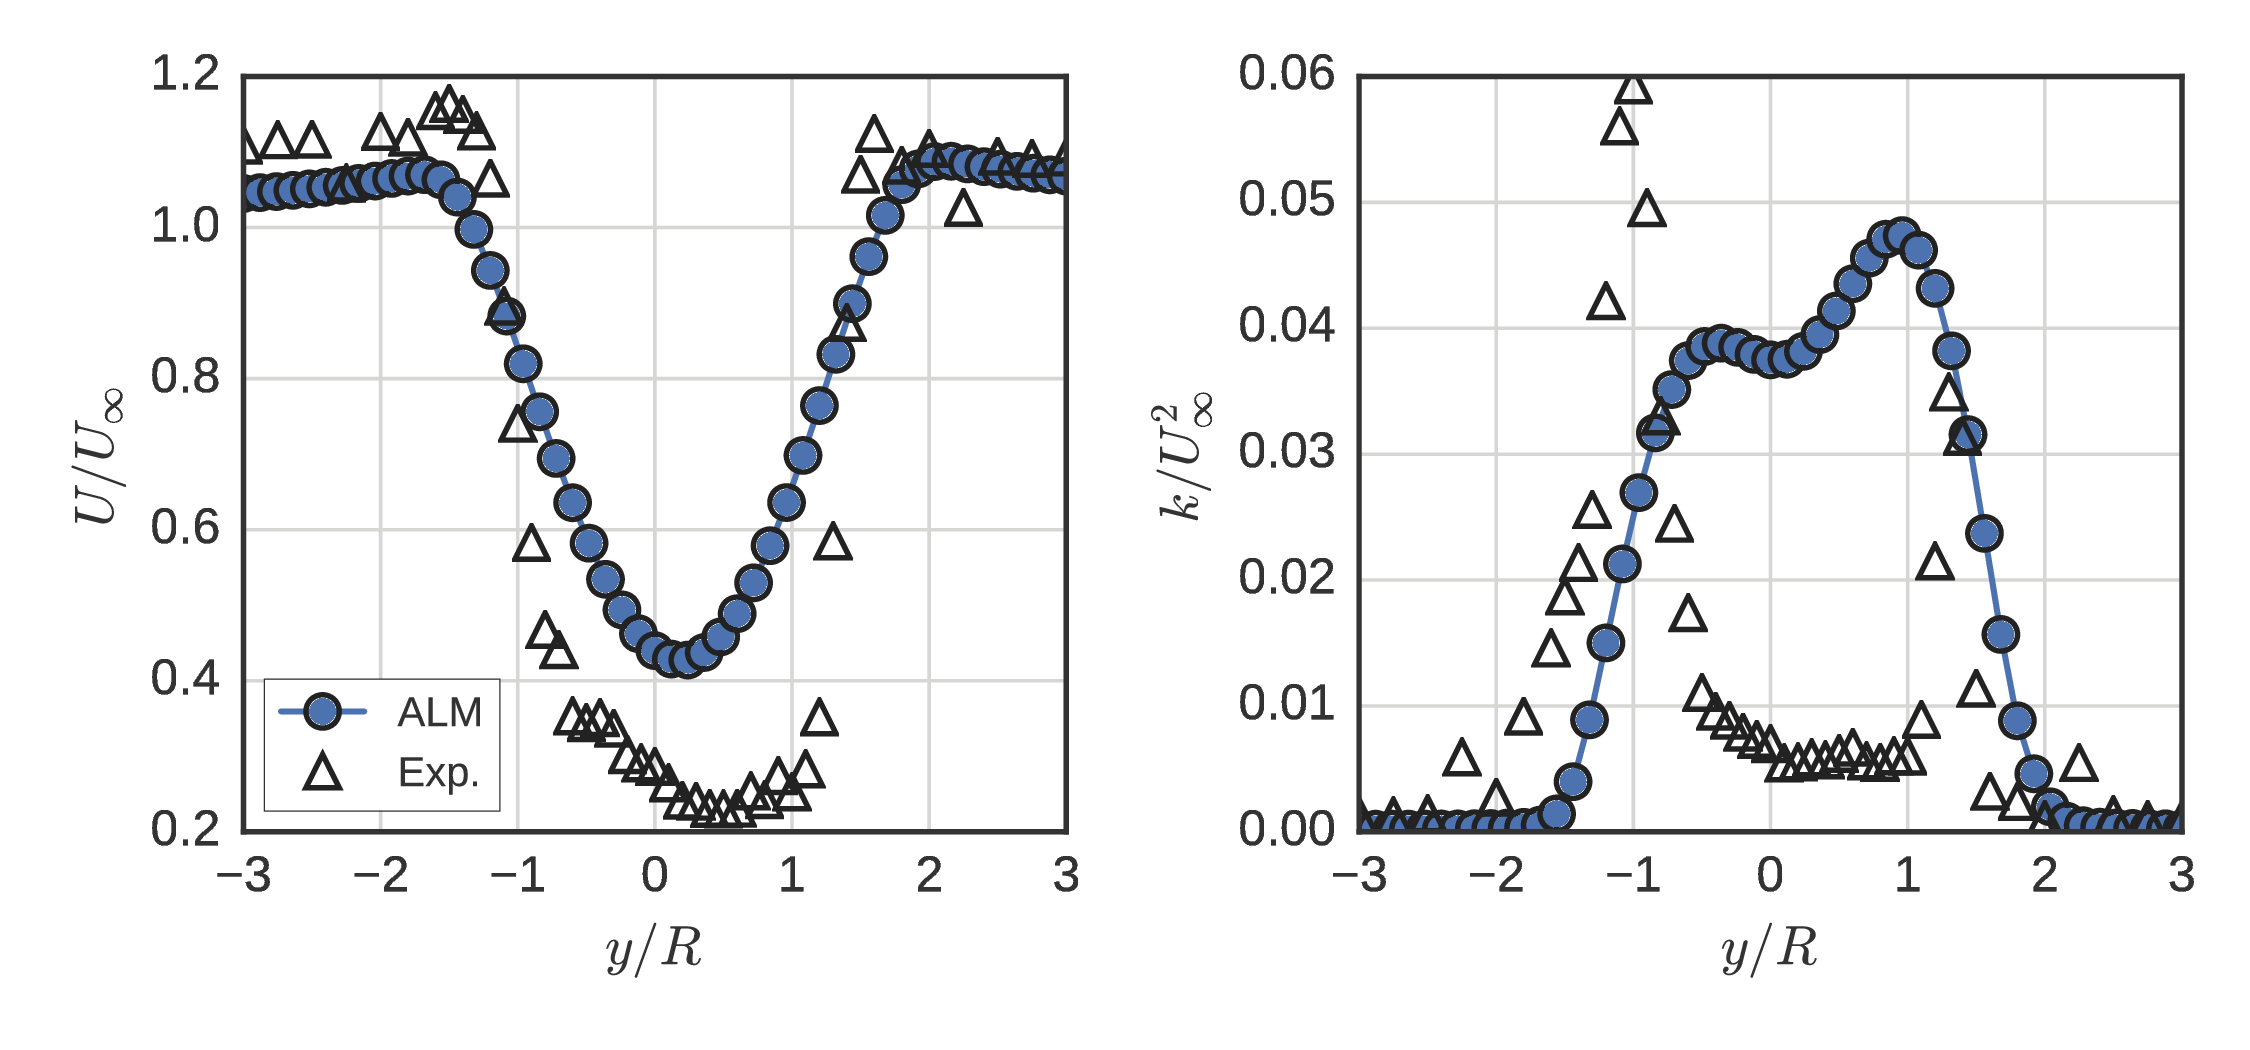
\includegraphics[width=0.85\textwidth]{RVAT-ALM_wake-profiles}
    
    \caption{Mean streamwise velocity (left) and turbulence kinetic energy
        (right) profiles at $z/H=0$ for the UNH-RVAT ALM.}
    
    \label{fig:RVAT-ALM-profiles}
\end{figure}

Weighted averages for the momentum recovery terms were computed identically as
they were in Chapter~\ref{chap:CFD}, and are plotted in
Figure~\ref{fig:RVAT-ALM-recovery} along with the 3-D blade-resolved RANS
results and experiments. The most glaring discrepancy is the ALM's prediction of
positive cross-stream advection, which is caused by the lack of detail in the
tip vortex shedding. The total for vertical advection, however, is close to that
predicted by the 3-D blade-resolved Spalart--Allmaras model. Levels of turbulent
transport due to eddy viscosity and deceleration due to the adverse pressure
gradient are between those predicted by the 3-D blade-resolved $k$--$\omega$ SST
and SA models. Overall, however, one might expect the total wake recovery rate
to be comparable between all models, which suggests the ALM would be an
effective tool for assessing downstream spacing of subsequent turbines, though
any blade--vortex interaction of very tightly spaced rotors would likely not be
captured.

\begin{figure}
    \centering
    
    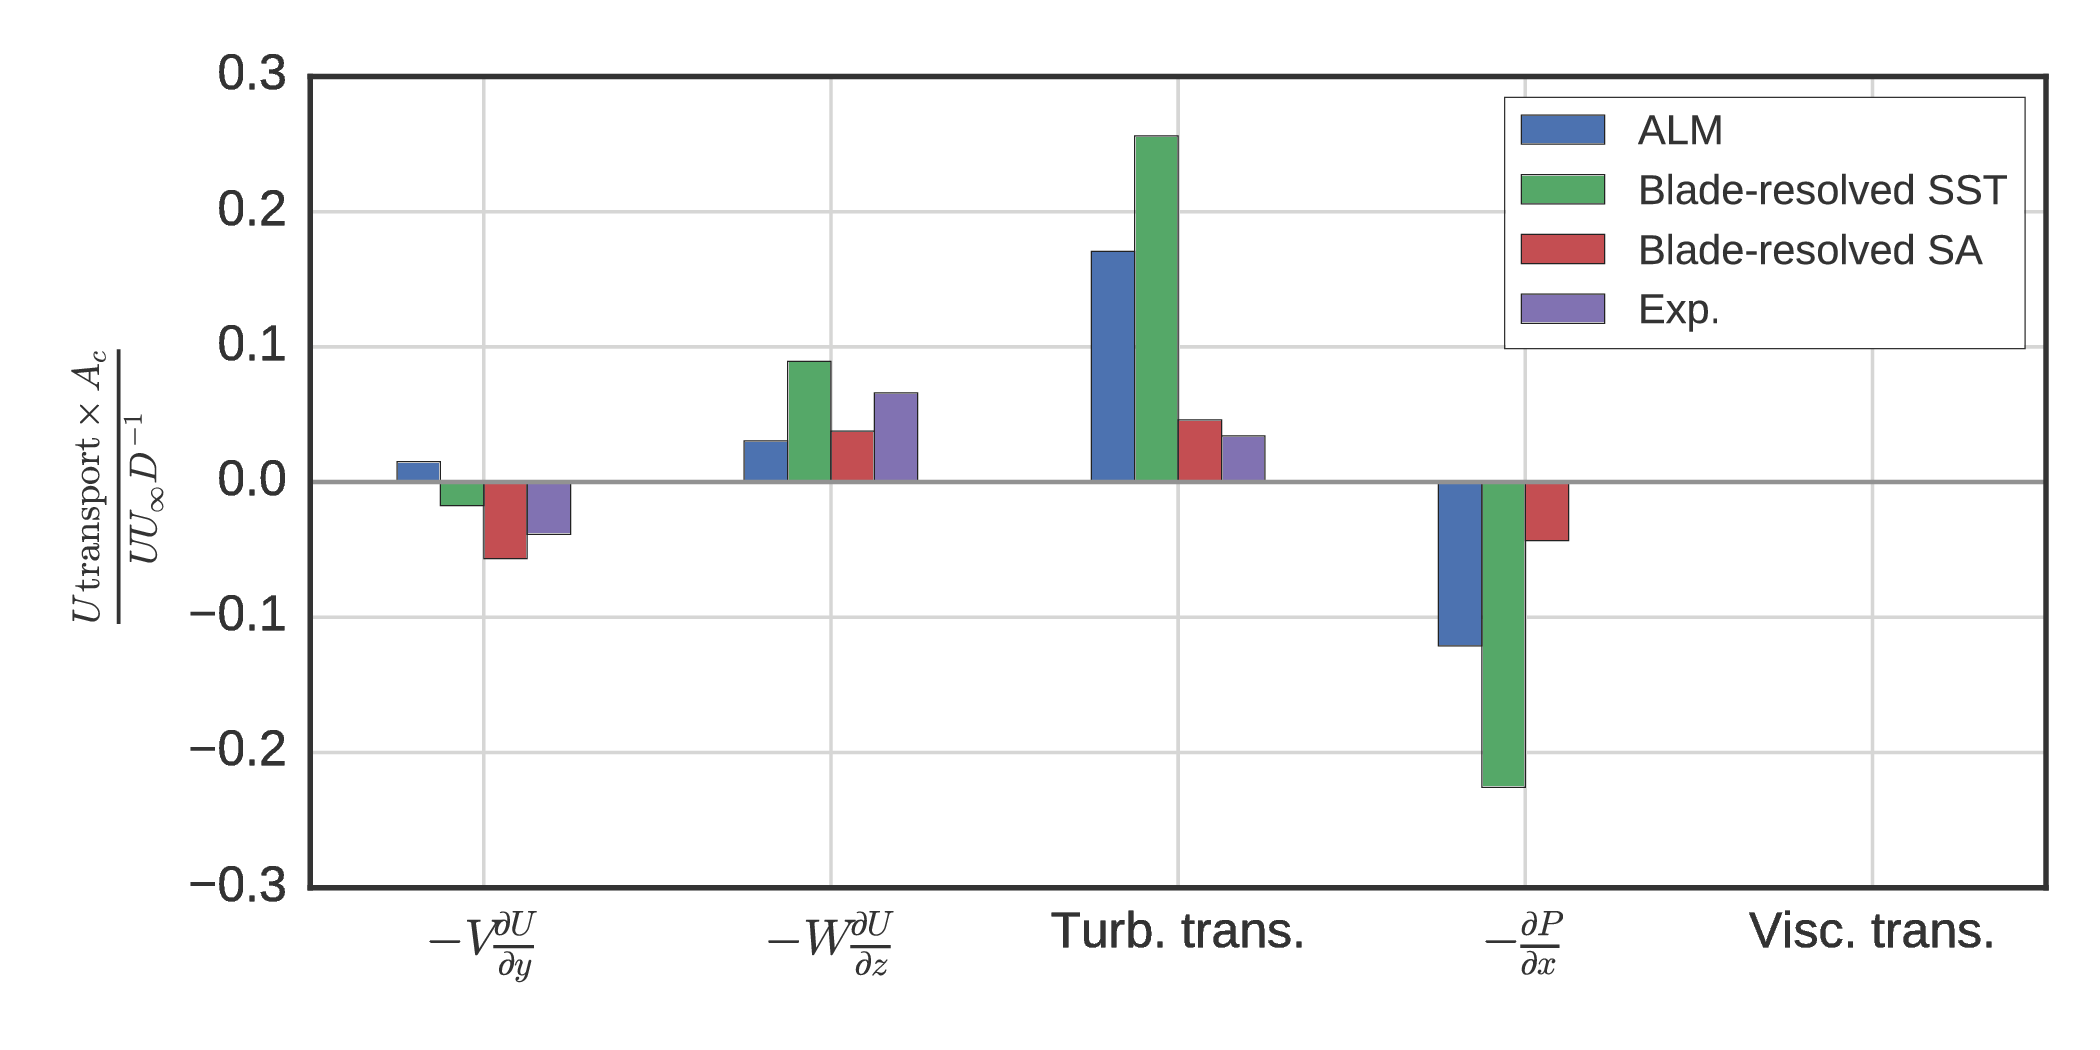
\includegraphics[width=0.85\textwidth]{RVAT-ALM_recovery-bar-chart}

    \caption{Weighted average momentum recovery terms for the UNH-RVAT actuator
        line model with a $k$--$\epsilon$ RANS closure, the two 3-D blade resolved
        RANS models described in Chapter~\ref{chap:CFD}, and the experiments in
        Chapter~\ref{chap:RVAT-baseline}}.
    
    \label{fig:RVAT-ALM-recovery}
\end{figure}


\subsection{RM2 RANS}

Figure~\ref{fig:RM2-ALM-perf-curves} shows the performance curves computed for
the RM2 by the ALM, and those from the tow tank experiments. As with the high
solidity RVAT, the drop in $C_P$ comes at higher $\lambda$.

\begin{figure}
    \centering
    
    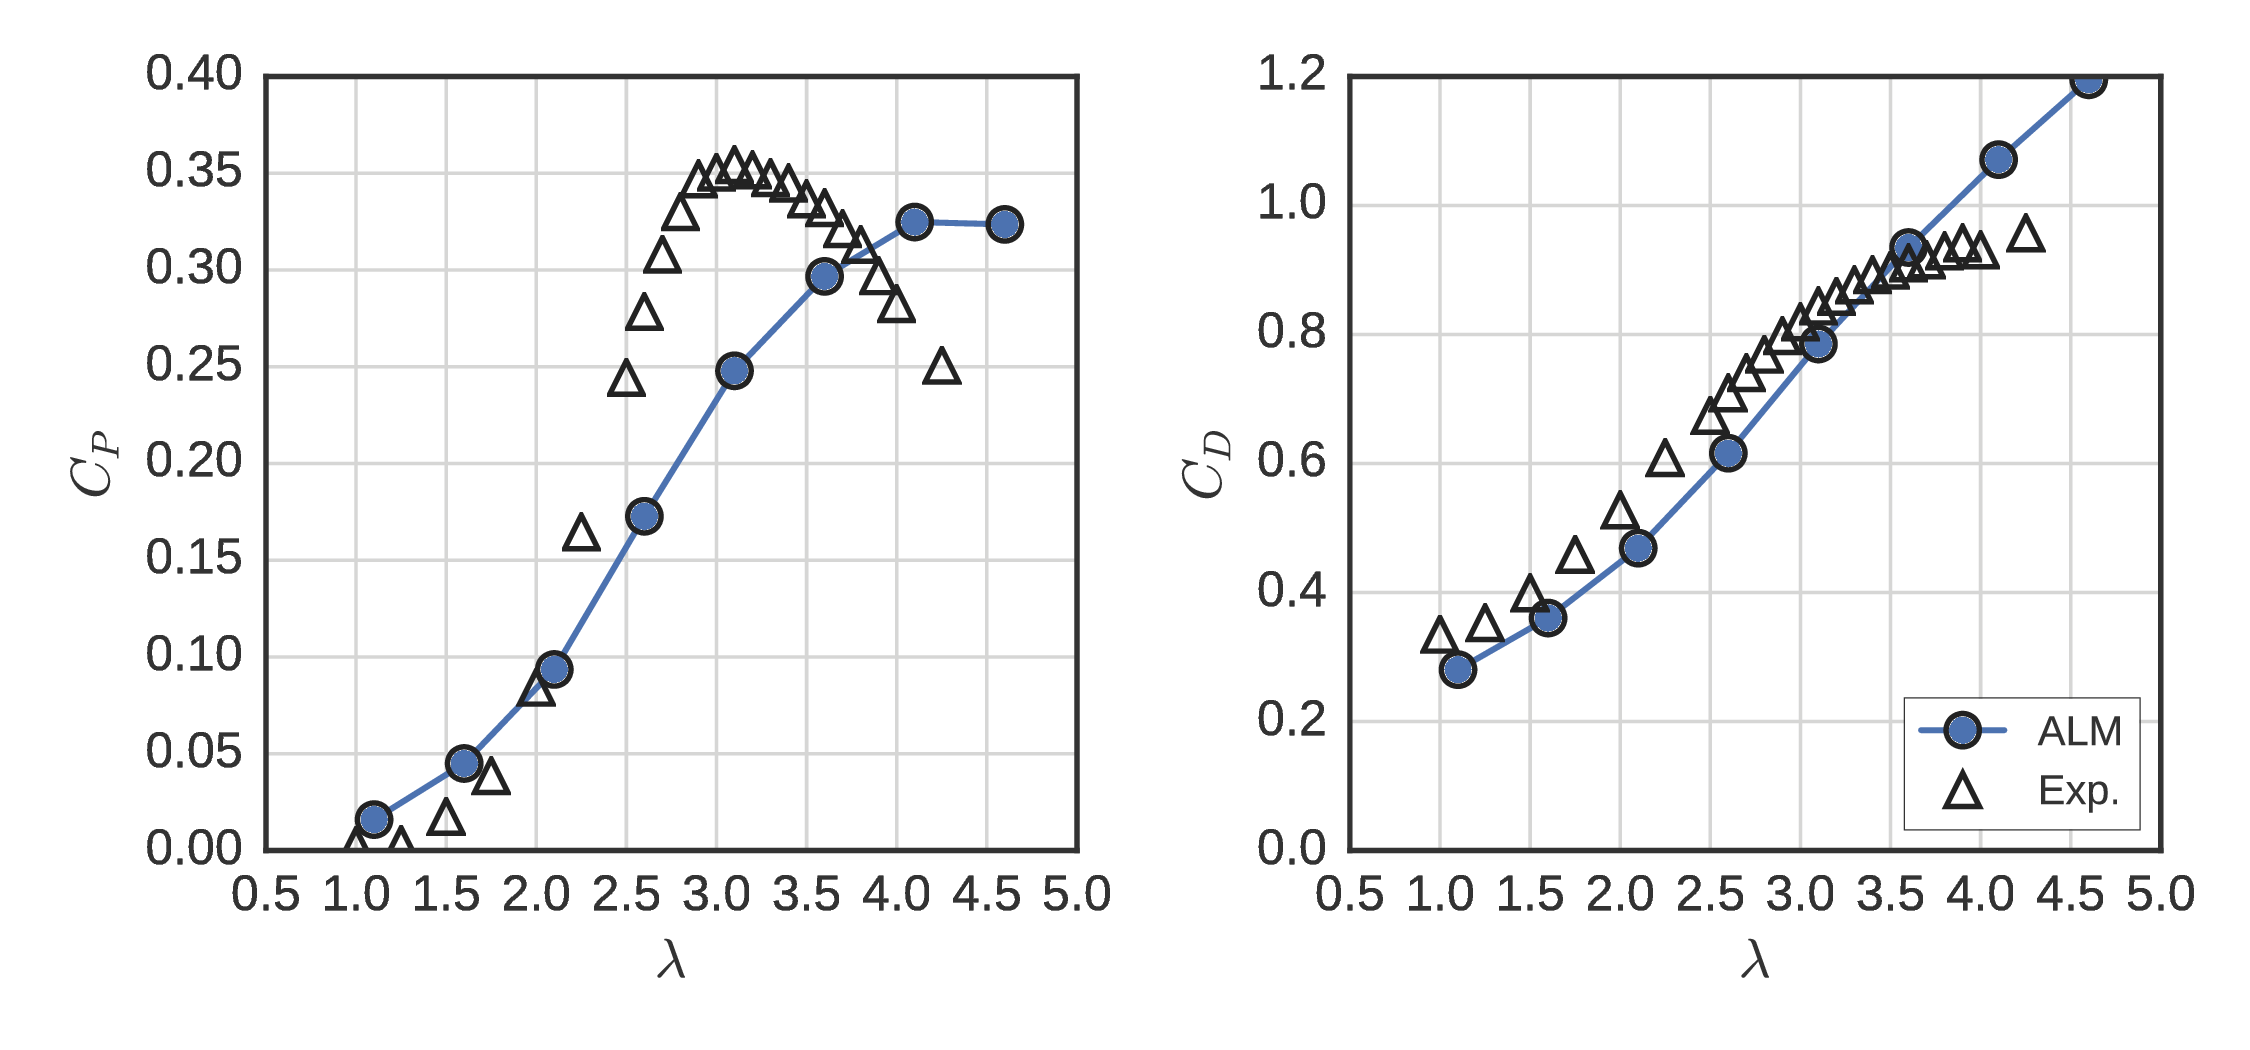
\includegraphics[width=0.85\textwidth]{RM2-ALM_perf-curves}
    
    \caption{Power and drag coefficient curves computed for the RM2 using the
        ALM.}
    
    \label{fig:RM2-ALM-perf-curves}
\end{figure}

Figure~\ref{fig:RM2-ALM-meancontquiv} shows the mean velocity field computed
by the ALM for the RM2.

\begin{figure}
    \centering
    
    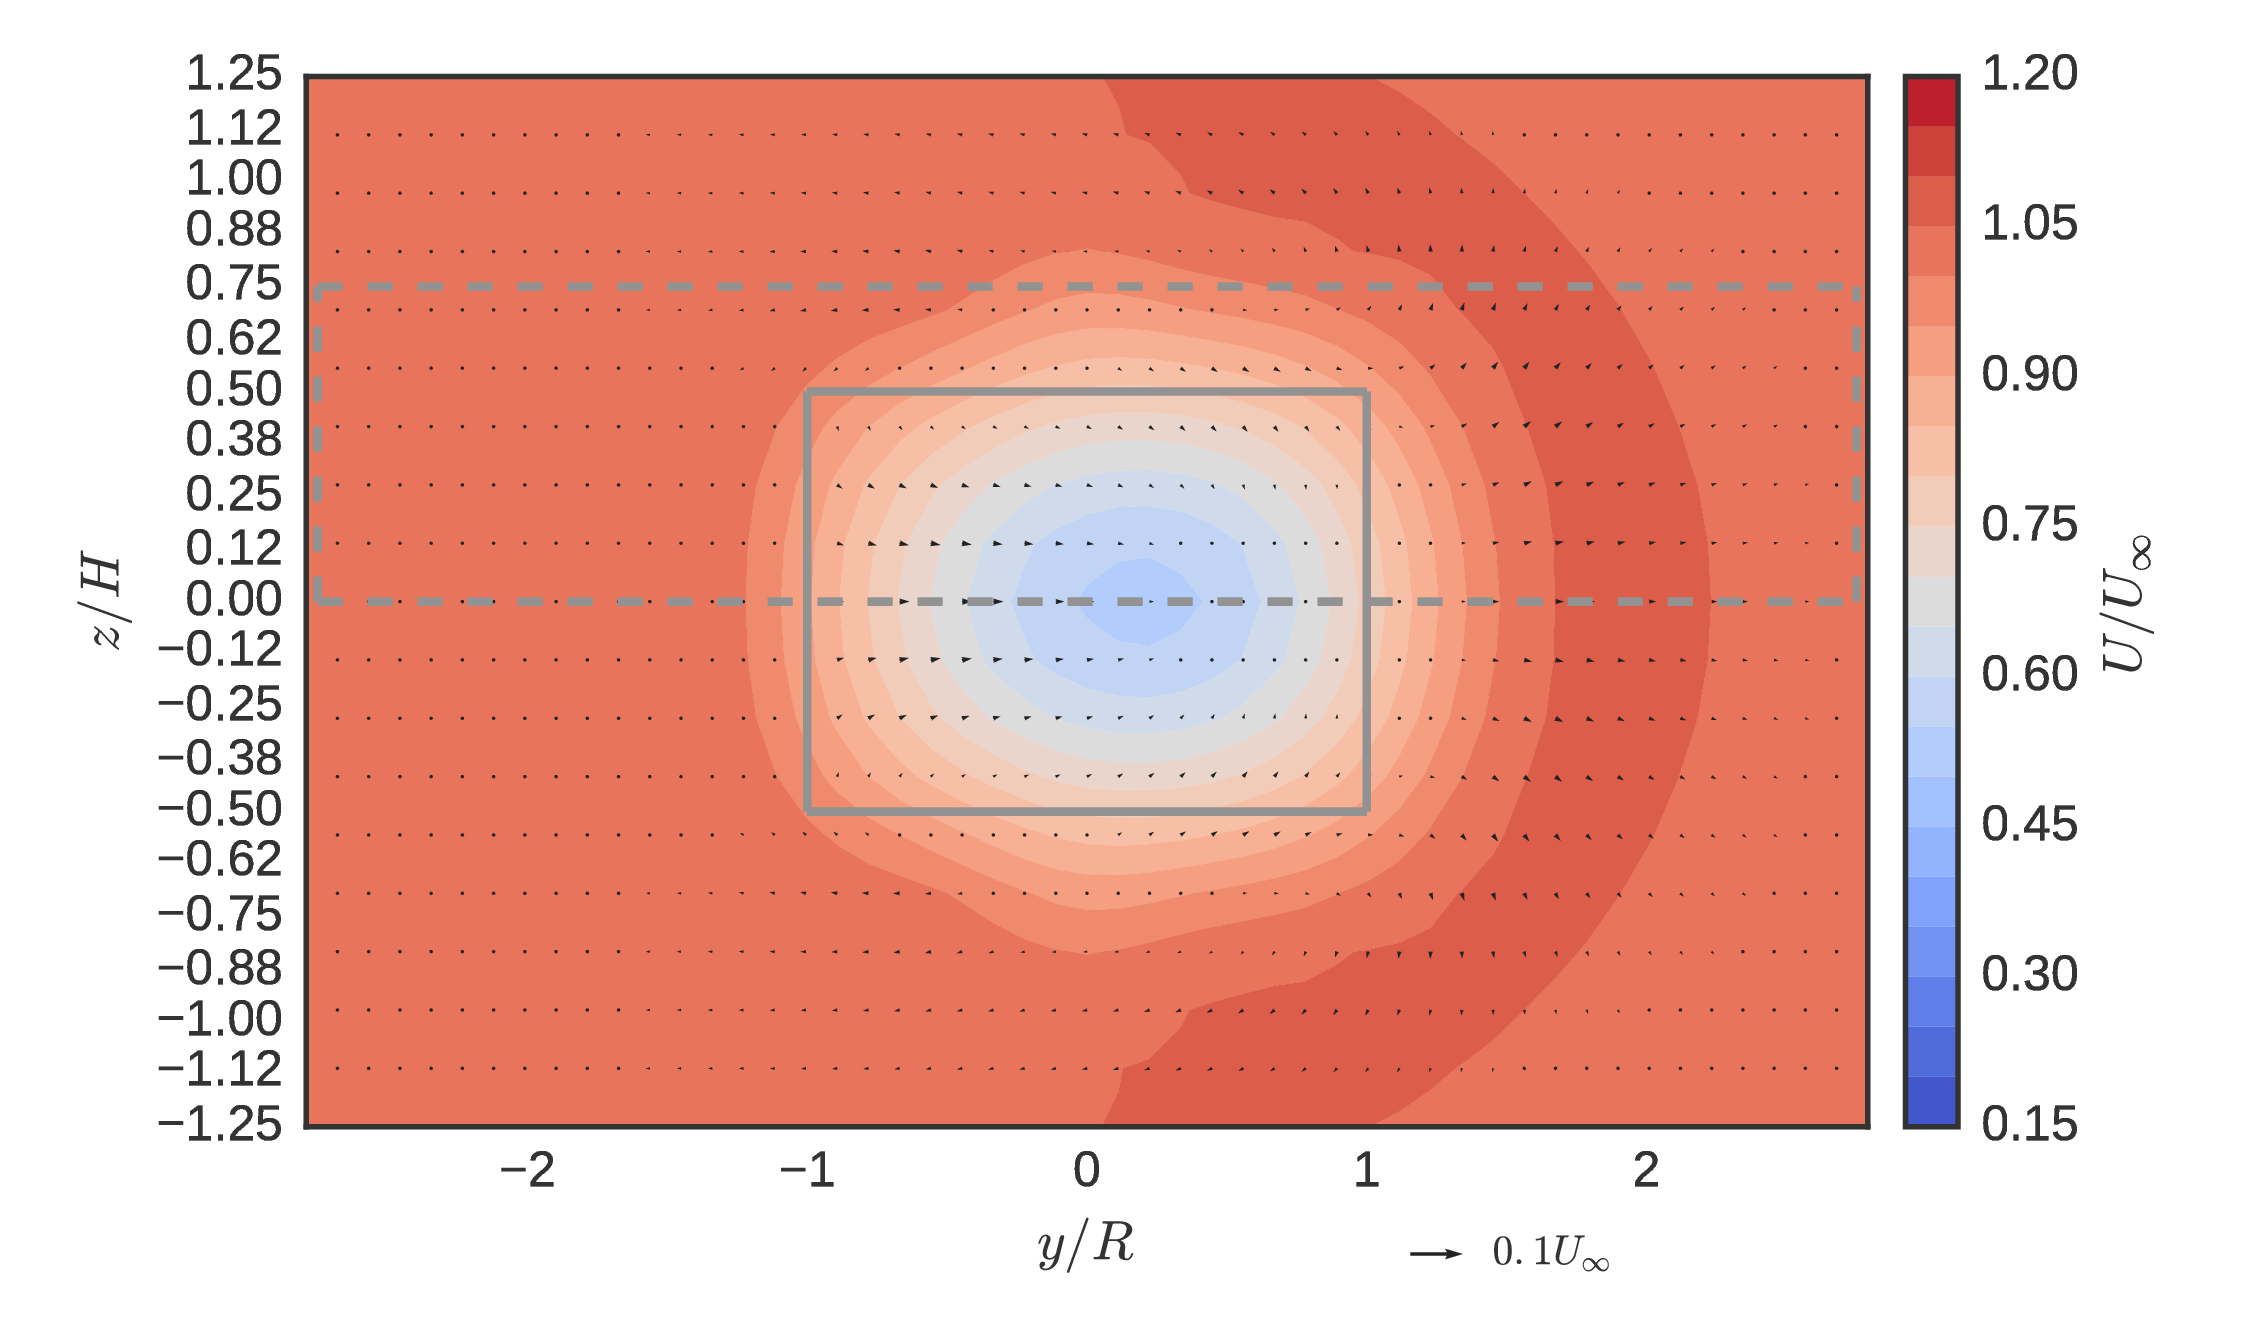
\includegraphics[width=0.9\textwidth]{RM2-ALM_meancontquiv}
    
    \caption{Mean velocity field at $x/D=0.93$ for the RM2 predicted by the
        ALM.}
    
    \label{fig:RM2-ALM-meancontquiv}
\end{figure}

Figure~\ref{fig:RM2-ALM-kcont} shows the ALM's turbulence kinetic energy
predictions in the near-wake of the RM2. Like for the UNH-RVAT, $k$ appears to
be concentrated on the $+y$ side of the rotor. However, overall levels of
turbulence are lower than for the UNH-RVAT, which is consistent with the
experimental results.

\begin{figure}
    \centering
    
    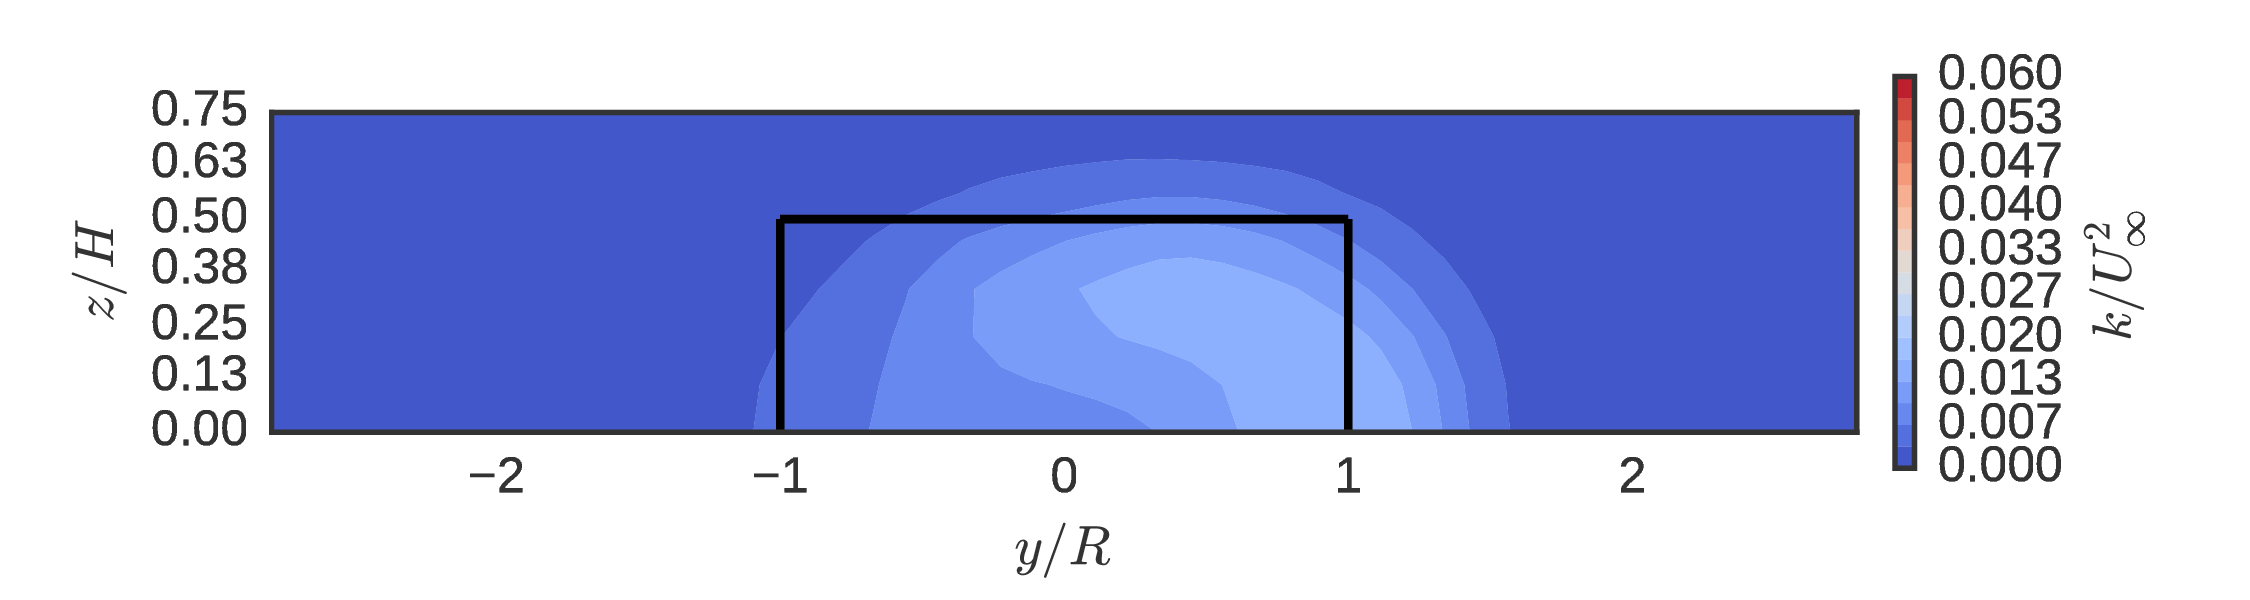
\includegraphics[width=0.9\textwidth]{RM2-ALM_kcont}
    
    \caption{Turbulence kinetic energy contours at $x/D=0.93$ behind the RM2
        predicted by the ALM.}
    
    \label{fig:RM2-ALM-kcont}
\end{figure}

\begin{figure}
    \centering
    
    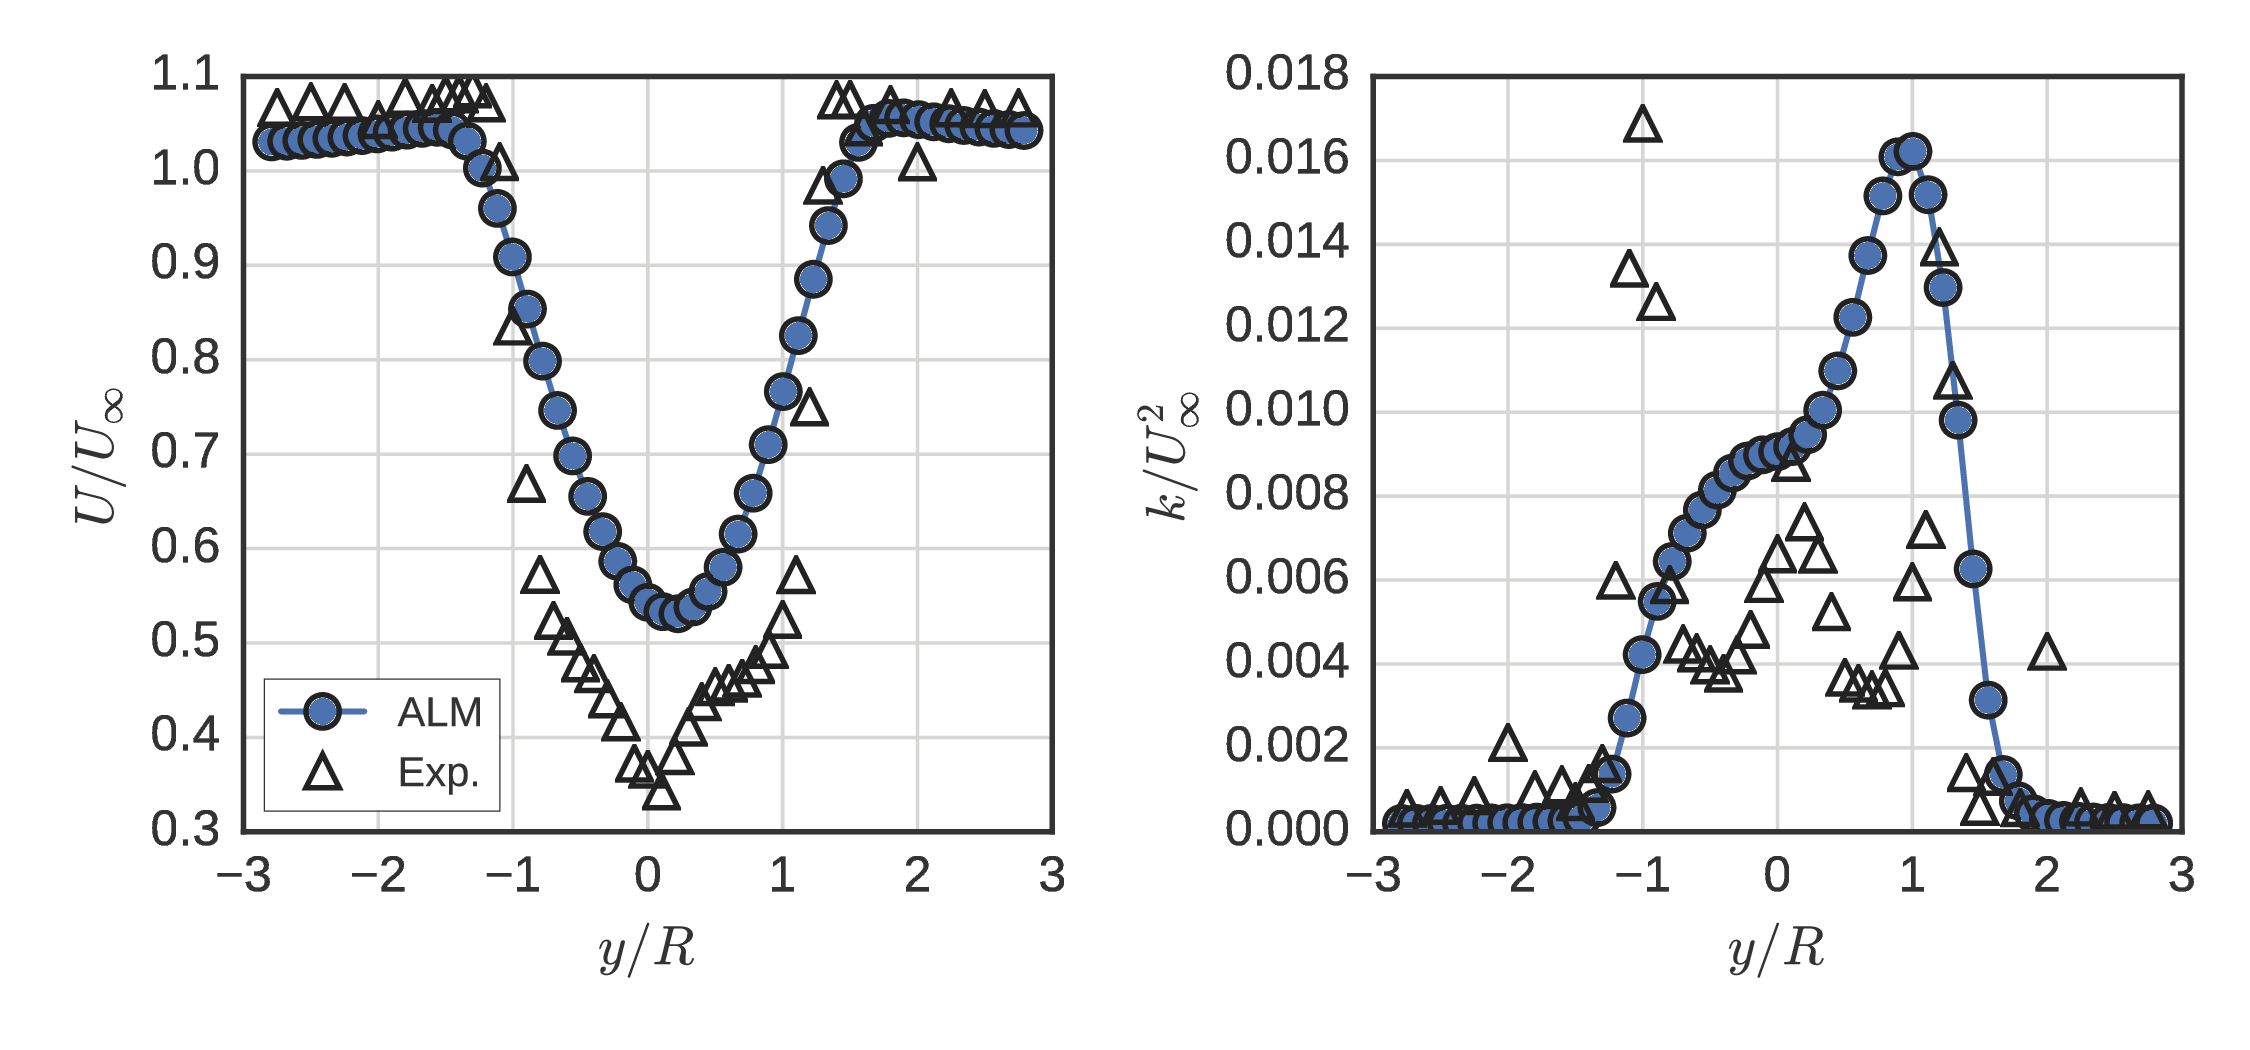
\includegraphics[width=0.85\textwidth]{RM2-ALM_wake-profiles}
    
    \caption{Mean streamwise velocity (left) and turbulence kinetic energy
        (right) profiles at $x/D=0.93$ and $z/H=0$ for the RM2 ALM.}
    
    \label{fig:RM2-ALM-profiles}
\end{figure}

\begin{figure}
    \centering
    
    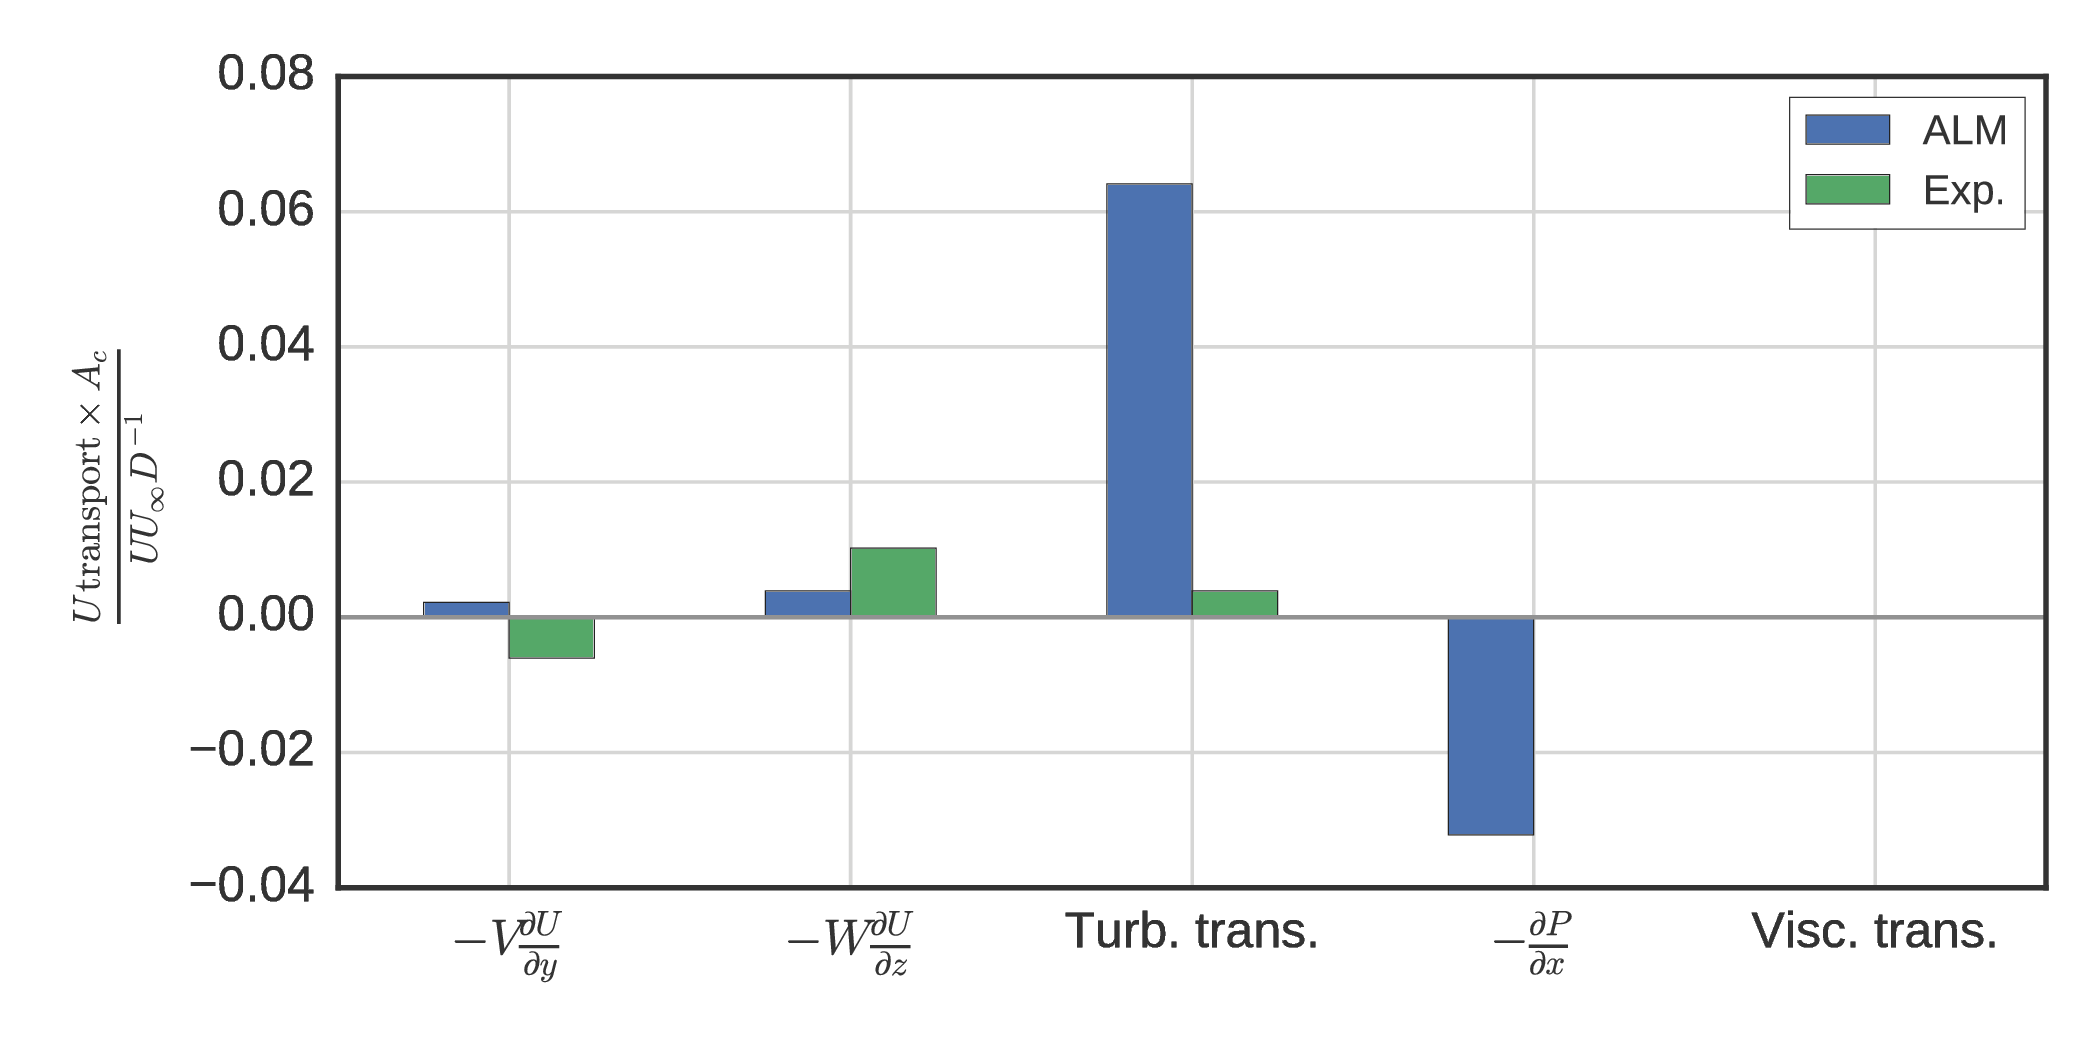
\includegraphics[width=0.85\textwidth]{RM2-ALM_recovery-bar-chart}
    
    \caption{Weighted average momentum recovery terms at $x/D=0.93$ for the RM2
        actuator line model with a $k$--$\epsilon$ RANS closure and the experiments
        described in Chapter~\ref{chap:RM2}}.
    
    \label{fig:RM2-ALM-recovery}
\end{figure}


\subsection{UNH-RVAT LES}

Since this was the most interesting wake structure...

Since the computational cost of LES is significantly higher than RANS,
verification was not performed. Instead, mesh resolution was chosen relative to
similar studies of turbine wake ALM. Of the studies surveyed
\cite{Shamsoddin2014,Archer2013,Martinez-Tossas2015a,Troldborg2007}, the mesh
resolution ranged from 18--64 points per turbine diameter. The mesh here was set
accordingly by using a 16 point per meter base mesh, and refining twice in a
region containing the turbine to produce a 64 point per turbine diameter/height
resolution. The solver was run with a 0.002 second time step, which is
significantly within the limit described by \cite{Martinez-Tossas2015}, where an
actuator line element may not pass through more than one cell per time step.

For the LES, the default Smagorinsky model coefficients were used. 

As a look towards the future prospect of simulating large CFT arrays in great
detail, a single CFT was placed in a large eddy simulation (LES). Turbine
geometry was identical to the UNH-RVAT case, but the domain was extended to look
at wake evolution father downstream.

\begin{figure}
    \caption{Snapshot of vorticity contours for the UNH-RVAT LES case.}
    
    \label{RVAT-LES}
\end{figure}

\todo[inline]{Add meancontquiv for RVAT LES case?}


The planar weighted sum of streamwise momentum recovery terms was computed in
the same was as for the RANS cases with the exception of the turbulent transport
term, which for the LES was computed from the $x$-component of the divergence of
the Reynolds stress tensor:
\begin{equation}
    \text{Turb. trans.} = -\frac{\partial}{\partial x_j}
    \overline{u^\prime u^\prime_j},
\end{equation}
where $U$ and $u$ (without subscripts) indicate streamwise components.

\todo[inline]{Add recovery terms for RVAT LES case?}


\section{Computational cost}

\todo[inline]{Move this section to conclusions or top-level results section like
    CFD chapter.}

Compared to blade-resolved RANS, the ALM can solve a standalone turbine case on
the order of CPU minutes per second of simulated time versus 1,000 CPU hours per
second---a savings of 4 orders of magnitude. However, the results for the ALM
are not quite as detailed. For example, the $-y$ tip vortex (where dynamic stall
is occurring) is not captured by the ALM.

The RANS simulations took "$O(0.1)$ CPU hours per second of simulated time,
while the LES took $O(10)$.


\section{Conclusions}

In this chapter the actuator line model has been developed and tested against
the cross-flow turbine validation datasets acquired in previous chapters.

Despite a small loss in accuracy, the ALM can do a reasonable job predicting the
performance and wake of a cross-flow turbine. It is therefore expected that this
tool will provide a much improved means of designing array layouts compared with
simple actuator disks, point sources, or superposition techniques---and all with
acceptable computational cost, i.e., not requiring HPC resources.

The ALM provides a more physical flow description compared to momentum and
vortex models, at a reasonable cost. The ALM has an important advantage over
vortex methods in that the computational expense is mainly due to solving the
flow field, which remains reasonably constant, where vortex methods increase in
computational complexity each time step. This is especially important for array
simulations, where for a given domain adding many turbines will be cheap in the
ALM compared to the rapidly increasing number of vortex elements generated by
each turbine. The ALM also drastically reduces computational effort compared to
blade-resolved CFD, while maintaining the unsteadiness of the wake not resolved
by a conventional actuator disk.

However, the mean flow structure and turbulence generation due to blade tip and
dynamic stall vortex shedding shows some discrepancy with experimental and
blade-resolved CFD. Extensions to the ALM to deal with these shortcomings should
be developed, e.g., a turbulence injection model as developed by James \emph{et
    al.} \cite{James2010} or a model that will ``turn'' the ALM body force vectors
to approach the effects of leading and trailing edge separation during dynamic
stall.

Thanks to the ALM's general implementation as a source term in OpenFOAM flow
solvers, the same model was run inside a higher fidelity large-eddy simulation.
The modular nature of the ALM using OpenFOAM's \texttt{fvOptions} framework
means that as turbulence modeling and computational power advance, the ALM can
continue to be used.

%%% Below from proposal introduction

If the proposed body force model is inadequate for postdicting our experimental
performance data, one possible strategy for improving accuracy is to generate
foil coefficient databases with more dimensions, e.g., blade pitch rate or local
turbulence levels. It may also be possible to modify the dynamic loading models
based on insight from the body-fitted grid simulations.

%%% End from proposal introduction

At the very least, the prospect of using ALM simulations to drive down
computational cost of RANS by nearly five orders of magnitude justifies further
development.

At contemporary levels of computing power, the ALM is a useful tool when HPC is
not feasible. Furthermore, if arrays of CFTs become make it to commercial scale,
the ALM combined with LES represents one of the highest fidelity tools
available.

From an engineering standpoint, the ALM was successful at ranking the two
turbines' performance. $\lambda_0$ was identified well for the UNH-RVAT, as well
as its maximum $C_P$. For the RM2, which was expected to be easier to model
thanks to its lower $c/R$ ratio, $C_{P_{\max}}$ was computed well, though
$\lambda_0$ was not. However, it may be desirable to operate the RM2 at slightly
higher $\lambda \approx 3.5$ to mitigate the fatigue loading due to stall, where
$C_P$ is close to $C_{P_{\max}}$, and the ALM was more successful.


\section{Future work}

Since the ALM relies on static foil coefficient data, it is crucial that more be
measured and published openly, to allow the exploration of new turbine designs.
There is some doubt regarding the veracity of the Sheldahl and Klimas NACA foil
data \cite{Bedon2014}. However, competing datasets at large laboratory scale
Reynolds numbers are rare, even for the standard symmetrical foils. CFD may play
a role in generating new data, but models must be rigorously validated, given
the difficulty in predicting stall and its importance on CFT blade loading.

The effects of local turbulence levels on foil coefficient data could be a model
worth developing, since stall delay could affect loading significantly.

The ALM should next be validated with far-wake data and/or data from two CFTs
operating in proximity of each other.

A better Reynolds number correction for foil data could be developed---one that
can successfully reshape the coefficient curves for the shifting stall point.

Rotor angular speed control via generator models could be included to test the
effectiveness of various control schemes, e.g., sinusoidal $\lambda$ set points,
which have been shown in some cases to improve mean power coefficient.
\todo[inline]{Get some information and a citation about UW's work on CFT
    controls.}

The ALM should be evaluated for its use in modeling CFT arrays.

The ALM and its associated loading models could be used to develop dynamic wall
functions for coarse blade-resolved RANS, which would provide yet another option
for reduced computational expense.

Flow curvature corrections should be examined in more detail, and it may be
beneficial to develop models to transform entire foil datasets to match their
virtual camber, as suggested by Migliore \emph{et al.}~\cite{Migliore1980}.

Since \textit{turbinesFoam} is compatible with OpenFOAM's volume of fluid (VOF)
multiphase flow solver \textit{interFoam}, the ALM's effectiveness should be
assessed for predicting the generation and interaction of turbines with surface
waves. The ADV positioning system developed in Chapter~\ref{chap:exp-setup}
could be retrofitted with a wave staff to measure and validate the free surface
disturbance, which could be key to predicting the effects of placing turbines in
channels at high blockage ratio.

The effects of separation at blade--strut attachment points should be further
studied. This may be one reason the turbine performance is overestimated at high
$\lambda$, since these effects scale approximately with
$\lambda^2$--$\lambda^3$.


\subsection{Turbulence injection}

Conventional blade element simulations use either momentum or vortex methods to
solve for the incident flow field, but these methods do not model the effects of
turbulence. With the actuator line model, there is the opportunity to improve
the physical realism by not only adding a source term to the momentum equation,
but also to the turbulence model equations. James \emph{et al.} \cite{James2010}
implemented an actuator disk model in a RANS model with a $k$--$\epsilon$
closure, which ``injected'' $k$ and $\epsilon$ from the actuator disks to more
realistically simulate the turbine's turbulent wake and enhance momentum
transport. However, to the author's knowledge injecting turbulence quantities
has never been done in an actuator line model.

The primary goal was to develop a simple model that use blade loading to compute
turbulence values to inject locally into the $k$--$\epsilon$ RANS model scalar
fields. Initial targets for local turbulence levels were established by
simulating a 2-D symmetrical NACA 0021 airfoil at $Re_c = 2 \times 10^5$ using
the $k$--$\omega$ SST turbulence model, given its favorable reputation for
predicting stall. The model results for the specific dissipation $\omega$ were
converted to $\epsilon$ by \cite{Wilcox1994}
\begin{equation}
    \epsilon = \beta^* \omega k.
\end{equation}

A snapshot of the mesh for the 2-D blade-resolved static foil case is shown in
Figure~\ref{fig:NACA-foil-mesh}. 30 seconds of unsteady flow over the foil were
simulated using OpenFOAM's \textit{pimpleFoam} solver and averages were
calculated over the final 20 seconds. Mean turbulence quantities were sampled
along a vertical line at one chord length behind the quarter chord, and the
maximum turbulence scalar value was stored. The goal here was not necessarily to
find injection rates that would correspond to experiments, but rather those that
would occur in a blade-resolved RANS case, though our results from
Chapter~\ref{chap:CFD} indicate that for the $k$--$\omega$ RANS model these may
be equivalent.

\begin{figure}
    \centering
    
    \caption{2-D NACA 0021 foil mesh at 20 degrees angle of attack.}
    
    \label{fig:NACA-foil-mesh}
\end{figure}

Mean turbulence kinetic energy contours next to the foil are shown in
Figure~\ref{fig:NACA-foil-k} and the foil force coefficients and sampled mean
turbulence values are shown in Figure~\ref{fig:NACA-foil-coeffs}. There is a
clear correlation between drag and turbulence in the foil wake, though
turbulence levels seem to saturate around the static stall angle. These features
motivated the development of a simple linear model for turbulence injection rate
as a function of drag coefficient.

\begin{figure}
    \centering
    
    \caption{Mean turbulence kinetic energy computed around the 2-D NACA 0021
        foil at 20 degrees angle of attack.}
    
    \label{fig:NACA-foil-k}
\end{figure}

\begin{figure}
    \centering
    
    \caption{Simulated force coefficients and turbulence quantities plotted
        versus angle of attack for a 2-D NACA 0021.}
    
    \label{fig:NACA-foil-coeffs}
\end{figure}

Turbulence kinetic energy was regressed linearly against the drag coefficient up
to the static stall angle, which was determined numerically as the angle of
attack at which $C_d$ first increased at more than 0.02 per degree. For angles
above static stall, the average value of $k$ was taken to be the limit for
turbulence injection. The turbulent dissipation $\epsilon$ was regressed
linearly against $k^{3/2}$, which was motivated by the relationship from the
standard $k$--$\epsilon$ model \cite{Wilcox1994}:
\begin{equation}
    \epsilon = C_\mu \frac{k^{3/2}}{l},
\end{equation}
where $C_\mu$ is a closure coefficient, typically 0.09.

Figure~\ref{fig:NACA-foil-fits} shows the simulation results plotted along with
their associated fit lines. The regressions and their resulting parameters
inspired injection rates for $k$ and $\epsilon$ of the form
\begin{equation}
    k_s = C_k \frac{U^3}{c} \min \left[ k_{\max} ,\, | m_k C_d +
    b_k | \right],
\end{equation}
and
\begin{equation}
    \epsilon_s = C_\epsilon \frac{k_s^{3/2}}{c},
\end{equation}
respectively, where $C_k$ and $C_\epsilon$ are tuning constants, $U$ is the
relative velocity magnitude, $c$ is the actuator line element chord length, and
$m_k$ and $b_k$ are the slope and intercept of the $k$ versus $C_d$ regression.

\begin{figure}
    \centering 
    
    \caption{Simulation results and linear regression models plotted for the 2-D
        NACA 0021 blade-resolved CFD simulation.}
    
    \label{fig:NACA-foil-fits}
\end{figure}

In practice, the model injection rate coefficients were tuned by trial-and-error
to fit the turbulence kinetic energy contours measured in the experiment. From
this perspective, the blade-resolved static foil modeling served to help
identify scaling relationships, but was not used to determine the coefficients
used in the ALM.


% Conclusions
\chapter{Conclusions}

To help meet the need for more high quality cross-flow turbine performance and
wake data---especially for higher solidity rotors---an automated turbine test
bed was developed as part of UNH's wave and tow tank, which increased the number
of possible tows per experiment by an order of magnitude while improving
repeatability. Two ``large laboratory scale'' turbines ($\sim 1$ m scale) were
designed, built, and tested: the high solidity UNH-RVAT, and the medium solidity
DOE/SNL RM2.

A baseline performance and near-wake measurement dataset was acquired for the
UNH-RVAT. A new method for assessing wake recovery was developed by rearranging
the streamwise mean momentum and mean kinetic energy equations to examine their
streamwise partial derivatives \cite{Bachant2015-JoT}. Weighted averages of
these terms were calculated from experimental data to assess the relative
balance of various transport mechanisms. For the UNH-RVAT, it was shown that the
mean vertical advection dominated in the near-wake region, which is caused by
the unique vorticity field generated by the bound and tip vortices.

Scale, or Reynolds number effects on the UNH-RVAT data were examined by
remeasuring performance and near-wake data at multiple tow speeds. It was shown
that the measurements became nearly $Re$-independent at a turbine diameter
Reynolds number $Re_D \sim 10^6$, which provides a good guideline for keeping
physical model tests relevant to full scale behavior.

A similar experimental campaign was undertaken for the RM2. Reynolds number
dependence showed a similar threshold, though the performance retained weak
linear $Re$-dependence at the highest speeds tested. This effect was also seen
when inspecting the maximum geometric torque coefficient computed from 2-D
static foil coefficient data produced by the XFOIL viscous panel code. Since the
UNH-RVAT has a higher solidity or chord-to-radius ratio, and therefore higher
virtual camber, the Reynolds number independence of its performance---estimated
by the geometric torque coefficient calculation---is more dramatic. The
near-wake of the RM2 overall showed lower levels of streamwise recovery, though
mean vertical advection was still dominant. The turbulence was generated more
symmetrically due to the rotors higher operational tip speed ratio, caused by
its lower solidity.

A blade-resolved RANS CFD model was evaluated for its ability to postdict the
UNH-RVAT baseline data, using both 2-D and 3-D configurations, and the
Spalart--Allmaras and $k$--$\omega$ SST turbulence models. As expected, the 2-D
models overestimated performance due to higher blockage and lack of end effects.
The lack of the vertical dimension also made them poor predictors of overall
wake dynamics, which precludes their use for analyzing arrays of turbines like
the UNH-RVAT, despite the computational feasibility. The 3-D models performed
better, with the Spalart--Allmaras model postdicting mean performance closest to
the experimental results. Both models did a good job resolving the qualitative
features of the near-wake's mean velocity field. Overall, 3-D blade-resolved
RANS presents a potentially less expensive, though less trustworthy alternative
to $Re$-independent physical model testing. However, the cost of 3-D
blade-resolved CFD really depends on availability of high performance computing
resources, much like physical model testing depends on the availability of
experimental facilities.

Motivated by the prospect of reducing the computational cost of 3-D CFD
simulations, an actuator line model was developed for cross-flow turbines and
implemented in a standard $k$--$\epsilon$ RANS model. The ALM was coupled with a
Leishman--Beddoes type semi-empirical dynamic stall model, end effects
correction, flow curvature correction, and an added mass model. Both the
UNH-RVAT and RM2 turbines were modeled with the RANS ALM. The performance curve
for the UNH-RVAT was well-postdicted for tip speed ratios below that of maximum
power output, but overpredicted above. For the RM2, however, the shape of the
$C_P$--$\lambda$ curve was not modeled correctly, though the maximum predicted
power coefficient was close to that observed in the experiments. To address this
issue, it is recommended that a more rigorous validation be performed with
respect to the LB DS model time constants. It is hypothesized that tip speed
ratio dependent time constants may improve mean performance predictions.

Wake predictions with the RANS ALM matched some of the qualitative near-wake
flow field characteristics seen in experiments, e.g., the mean vertical
advection, and production of turbulence kinetic energy on the $+y$ or upwind
facing side of the rotor. Neither of these matched perfectly with experiments,
but did a much better job representing a CFT wake than a simple actuator disk,
with minimal additional computational effort.

The UNH-RVAT was also modeled using large eddy simulation with a typical
Smagorinsky subgrid-scale model. Inside the LES, the ALM's mean performance
coefficient predictions at $\lambda=\lambda_0=1.9$ dropped about five percentage
points compared with RANS. However, the LES was able to resolve some of the
important qualitative features of the near-wake's mean velocity field, i.e., the
apparent mean vortex pair created by the blade tip vortex shedding. On the other
hand, levels of turbulence were significantly lower than those measured in the
experiment, which is thought to be an effect of the subgrid-scale modeling
delaying vortex breakdown. Therefore, it is recommended that wake measurements
be taken further downstream, and deeper investigation of SGS modeling be
undertaken in order to recommend which LES model might be most effective for
modeling arrays of cross-flow turbines.

On the whole, the work described here helps engineers better select initial CFT
rotor concepts, along with which methods should be used to predict their
suitability. Full scale prototyping is still the ``gold standard,'' while
physical modeling at $Re_D \sim 10^6$ can be effective. Both of these methods
are expensive, so it may be desirable to use 3-D blade-resolved RANS, despite
also being expensive, and its uncertainty with respect to turbulence modeling.
The actuator line model presents a good alternative when budgets are
constrained, allowing turbines to be simulated in a 3-D Navier--Stokes model
with typical computing resources, i.e., dropping the expense by two to four
orders of magnitude versus blade-resolved CFD for LES and RANS, respectively.
For designing arrays of turbines, the ALM at present is probably the best
balance between cost and accuracy, as its computational expense can be adjusted
by the turbulence modeling fidelity. Furthermore, the effects of, e.g., a free
surface or temperature/density stratification can easily be incorporated into
ALM simulations, opening up many opportunities for future investigation.

The products of this research---datasets, processing code, CAD files, simulation
case files, and the newly developed ALM software library turbinesFoam---have
been made freely and openly available. Besides improving transparency and
reproducibility, the open research paradigm also accelerates progress through
collaboration, allowing researchers to build on each other's work rather than
start anew. Working openly has already improved this research thanks to external
contributions, and it will hopefully improve others' as time goes on.


\addcontentsline{toc}{chapter}{Appendix A: Sharing research outputs}
\chapter*{Appendix A: Sharing research outputs}

A secondary goal of all the work performed herein was to share the products in
an open and useful manner.

% Add Bibliography into table of contents
\addcontentsline{toc}{chapter}{REFERENCES}

\vspace{0.5in}

\begin{singlespace}
\bibliographystyle{abbrv}
\bibliography{library}
\end{singlespace}

\end{document}
